\documentclass[10pt, landscape, a4paper]{article}
% Include necessary packages
\usepackage{geometry}
\geometry{landscape} % Set document to landscape mode
\usepackage{multicol}
\usepackage{graphicx}
\usepackage{amsmath} 
\usepackage{amssymb}
\usepackage{ccicons}
\usepackage{hyperref}
\usepackage{enumitem}
\usepackage[dvipsnames]{xcolor}
\usepackage{titlesec}

% Title and subtitle configuration
\titleformat{\section}
    {\normalfont\large\bfseries}{\thesection}{1em}{}
\titlespacing*{\section}
    {0pt}{3.5ex plus 1ex minus .2ex}{2.3ex plus .2ex}
\pagestyle{plain}

% Set page margins
\geometry{top=.8cm, left=.8cm, right=.8cm, bottom=1.3cm}

% Set paragraph indentation
\setlength{\parindent}{0pt}

% Set path for assets
\graphicspath{{assets/}}

% Title with manual subtitle
\title{Human Computer Interaction Summary HS23 \\ \vspace{10pt} \large Written by Benjamin Gantenbein bgantenbein@ethz.ch}

\setlength{\columnsep}{8pt}
\raggedcolumns

% Custom commands
\newcommand{\E}[0]{\mathbb{E}}
\newcommand{\R}[0]{\mathbb{R}}
\newcommand{\sgn}[0]{\text{sgn}}
\newcommand{\argmin}[1]{\underset{#1}{\text{argmin}}}
\newcommand{\argmax}[1]{\underset{#1}{\text{argmax}}}

\begin{document}
\begin{multicols*}{3}

% Content
\date{}
\maketitle

\section{Introduction}

\textbf{Goal of course} is to understand principles of user-centered design and being able to apply these to practice.
Learn about the basic notions of Computational Design in HCI context. \medskip


\textbf{Moore's Law} \smallskip

Computational power grows exponentionally. Transistor count doubles every two years. Also with RAM and pixel densities. 
However: Human capabilities stay stable.\medskip

\textbf{Good System design} Accounts for human capabilities, human error and exceptional circumstances. \medskip

\textbf{Human Computer Interaction} \smallskip

Concerned with design, evaluation and implementation of interactive computing systems for human use. \medskip


\begin{center}
	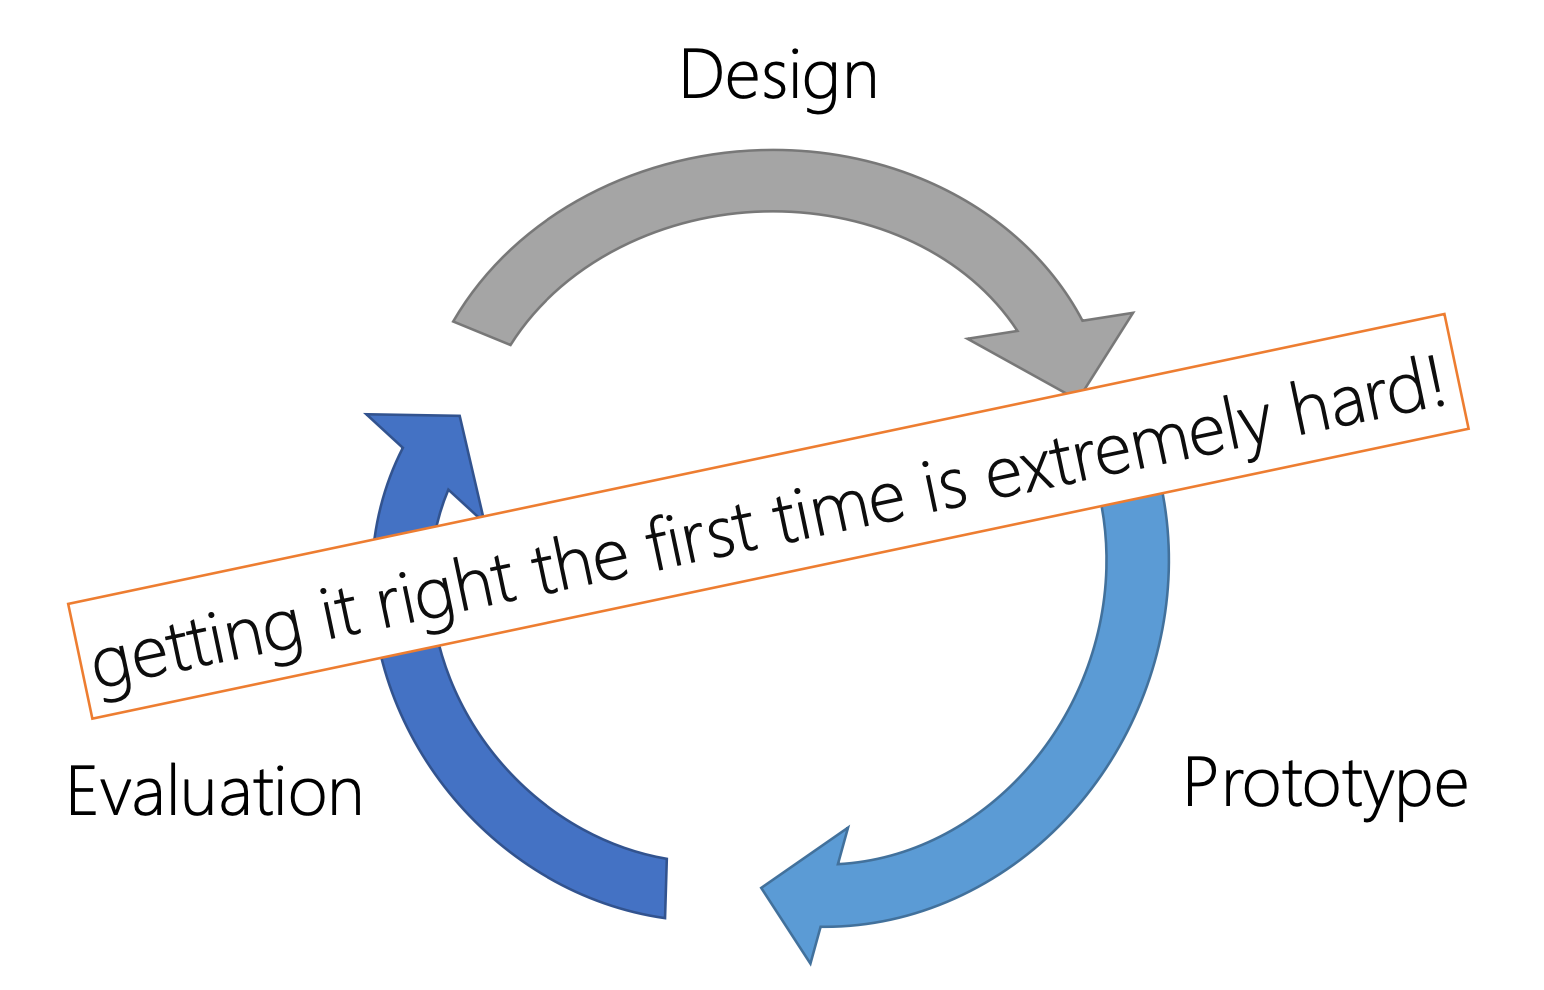
\includegraphics[width=\linewidth]{process.png}
\end{center}

\textit{Formative:} understand problem and user to inform our design. \medskip

\textit{Evaluative:} understand how well the design works. Also detects mistakes in design. \medskip



\section{User-centered Design}


\textbf{Design intention vs User Needs}

\textbf{Prototyping as an interative process}

\begin{center}
	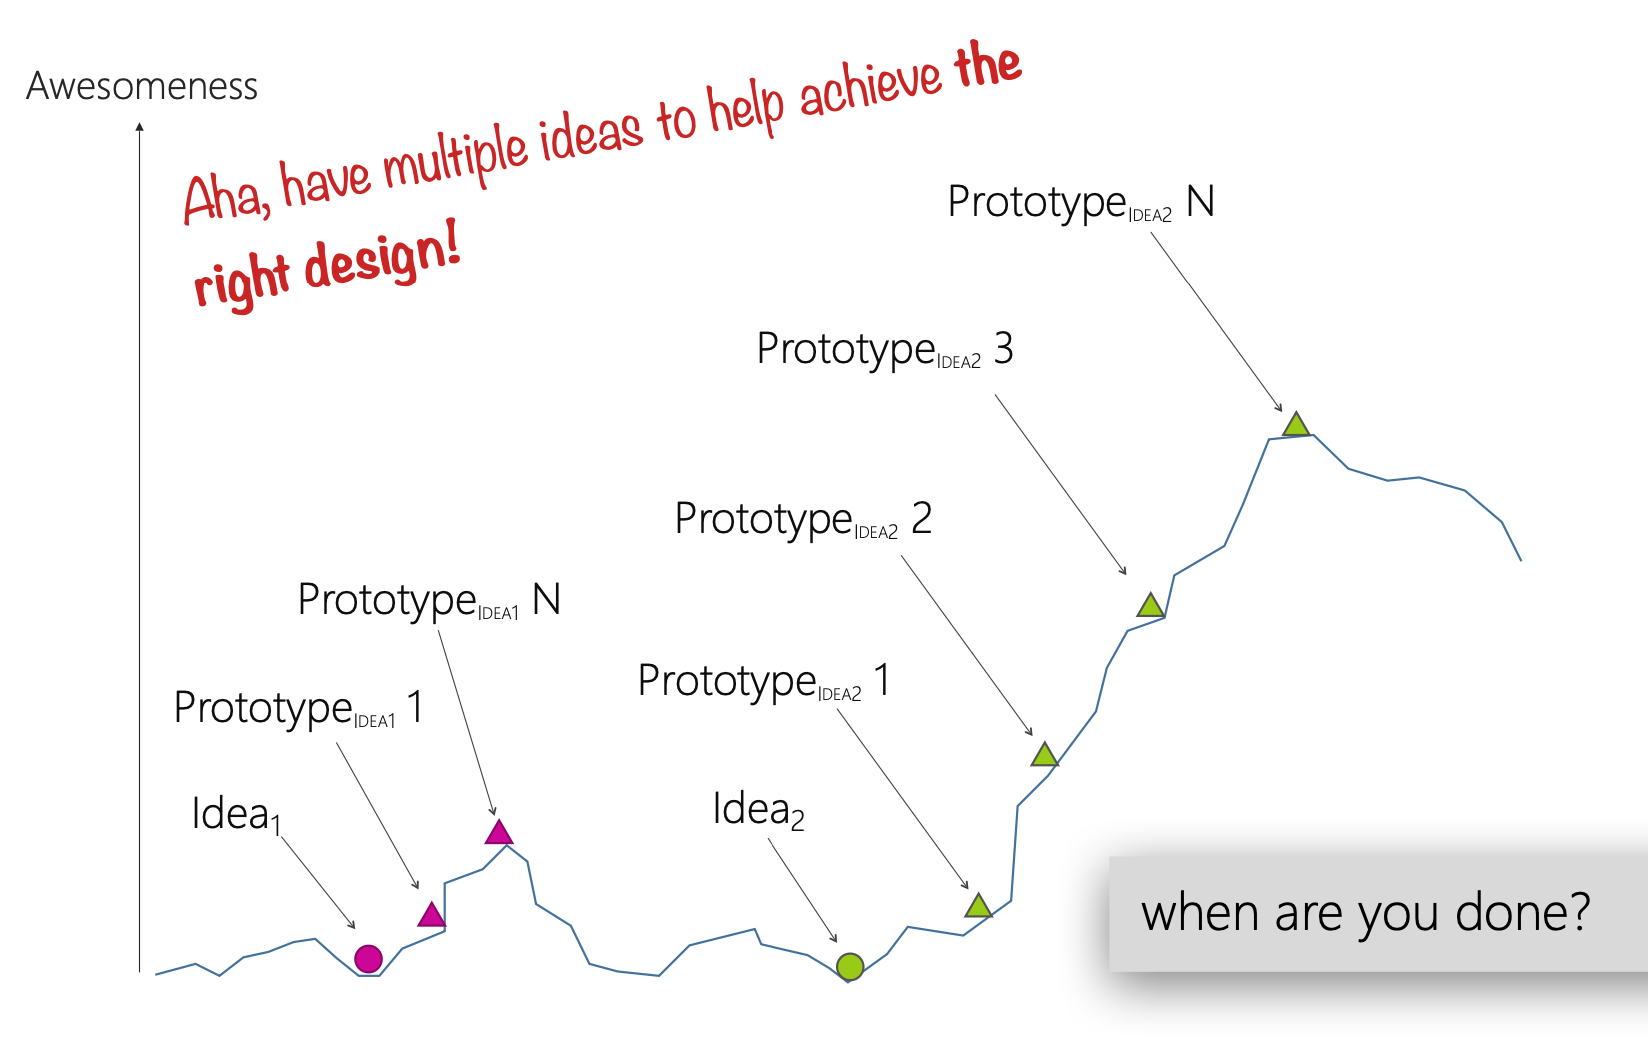
\includegraphics[width=\linewidth]{iterative_process.png}
\end{center}
Does the design work properly in the context of use? If not fix the problems and carry out more tests. \medskip

\textbf{Early focus on users and tasks:} Cognitive, behavioral, anthropomorphic AND attitudinal characteristics. \medskip

\textbf{Empirical Measurement:} Observe user's reactions and performance in scenarios, manuals simulations and prototypes, record and analyze. \medskip

\textbf{Root-Cause Analysis}
Problems need to be discovered (find the right problem to solve, not any problem to solve) and find the right solution to it. \medskip

\textbf{Need finding}

Users rarely know what they want. Cannot imagine what is possible. Instead look at tasks, context: 

\begin{multicols}{2}
    \begin{itemize}[itemsep=-5pt, topsep=-20pt, leftmargin=*]
	\item What information needed?
	\item Identify collaborators
	\item Why is task achieved the way it is?
	\item Identify tasks in existing behavior
	\item Identify tasks in future scenarios
	\end{itemize}
\end{multicols}

We ourselves are not representative of the typical user. To learn about customers conduct interviews, self-reports and logging/analytics.
Also observe users performing tasks and understand their cognition. \medskip

\textbf{Understanding the User}
Active observation is not knowing yet what you are looking for. 

\begin{multicols}{2}
    \begin{itemize}[itemsep=-5pt, topsep=-20pt, leftmargin=*]
	\item Immerse
	\item Observer
	\item Engage

	\end{itemize}
\end{multicols}


\begin{center}
	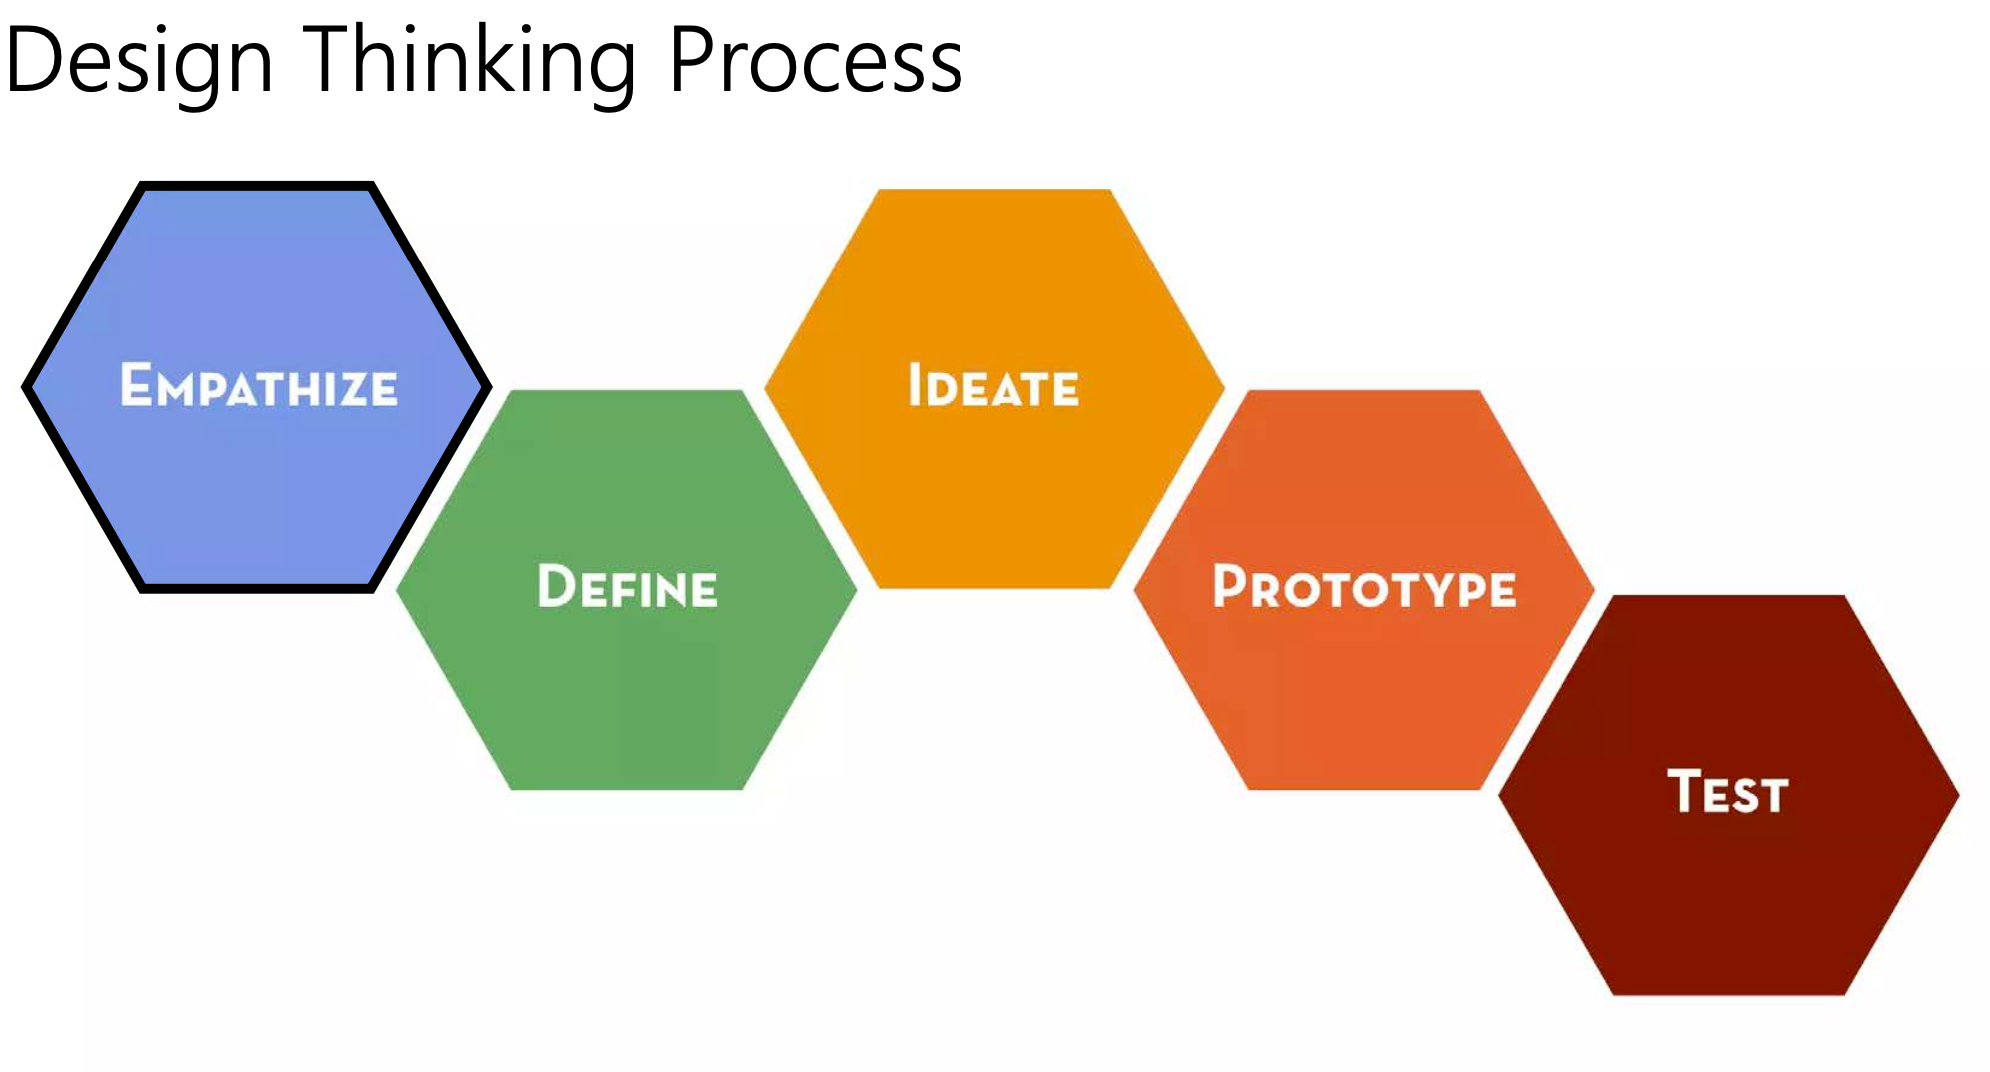
\includegraphics[width=\linewidth]{design_thinking_process.png}
\end{center}


\textbf{Goals of Need finding}


\begin{itemize}[itemsep=-5pt, topsep=3pt, leftmargin=*]
	\item Distill useful and actionable insights
	\item Make meaning from needfinding data
	\item reframe problem to guide solution search
\end{itemize}

\medskip

We start with closed ended questions and move to open ended questions: "What's and why's of feelings". Engage people in their environment.
The goal is to find inspiring users, that surprise us and bring us to gamge-changing ideas. \medskip

\textbf{Needs vs. features vs. requirements}

Requirements are goals that the system needs to accomplish. Solutions fulfill requirements. What does the user want to accomplish and how is he doing it?
What would they like to be doing? What are they currently disliking? For what is the system usable and what tasks will it support? Answering these questions will make the system more usable. \medskip

There are tons of methods to needfinding such as: 

\begin{multicols}{2}
    \begin{itemize}[itemsep=-5pt, topsep=-20pt, leftmargin=*]
	\item Task Analysis
	\item Interviews
	\item Affinity Diagrams
	\item Cognitive Walkthrough
	\item Questionnnaires
	\item Focus Groups
	\item Diary Studies
	\item "Speed dating"
	\item etc.
	\end{itemize}
\end{multicols}

\textbf{Interview}

Interviewee speaks 90 percent of time and stays on topic. We choose participants to be representative target users, either current or potential future users. We like both experts and typical users. Try to provide and explanation into how users make sense to themselves. \medskip

\textbf{Common pitfalls in interviews}
Suggesting answers. Hypthetical questions. \medskip

\textbf{Diary Study}
Ask people to record events as they happen. 

User diary studies for rare events, easily forgotton events and events where the actual frequncy is important. 

Problems with diary studies is that the simple tracking of their behaviors will change their behaviors. \medskip

\textbf{Retrospective Survey}
Ask about things happened in the past. Use this for critical events (well remembered), recent and memorable events, rare events that had a big impact an are memorable. DO not use them for hard to remember events.\medskip

\textbf{Artifact Analysis}
Look at things people leave around to understand a problem they might have. Use this for physical spaces (physical artifacts from workflows), tasks involving artifacts and interactions generating artifacs (emails, social media posts etc.).
Only use if there are in fact artifacts and there is no faster way to learn information. \medskip

\textbf{Contextual Inquiry}
Ethnographics or participatory design, combining aspects of other methods. Interviewing, observing in the context of work. Goal is to discover real requirements of the work.
Interview people while they are working and gather real artifacts. User decides the tasks, but you decide the focus. \medskip

\textbf{Key Differences}


\begin{center}
	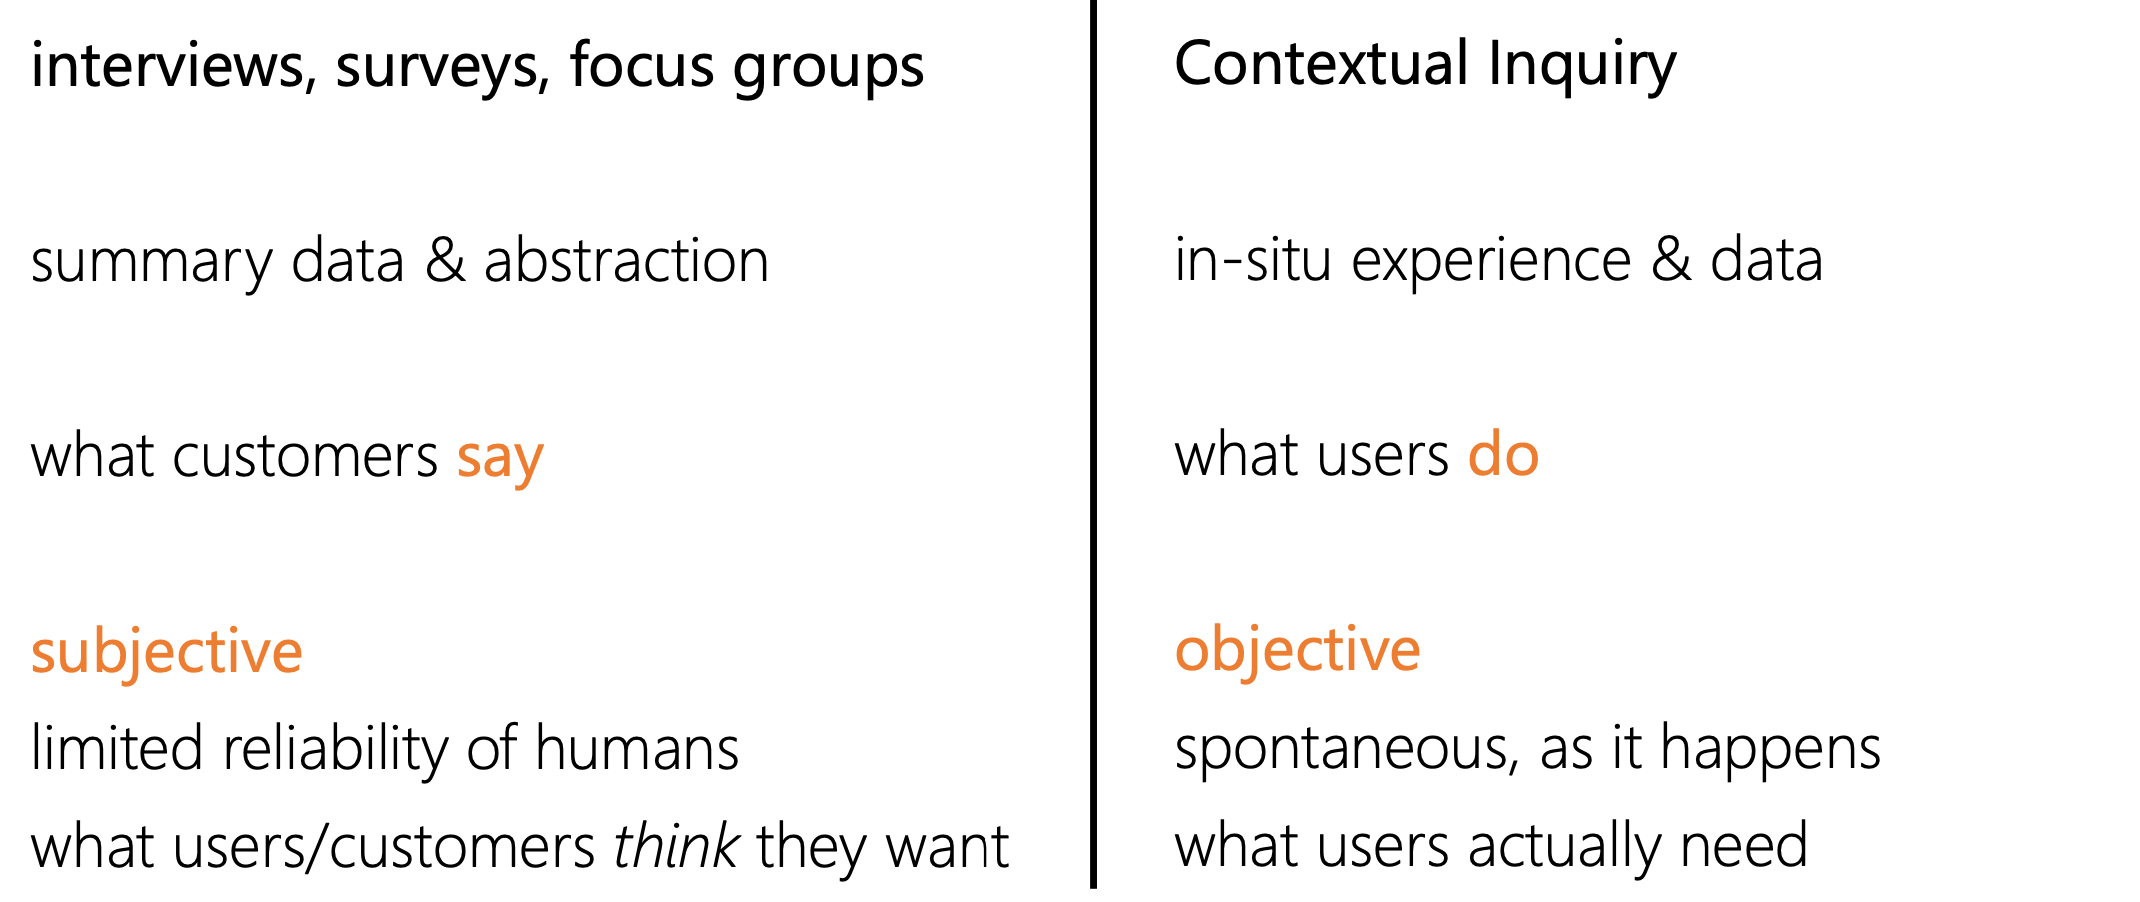
\includegraphics[width=\linewidth]{differences.png}
\end{center}

\textbf{Result of Need-Finding}
We know what works and what does not yet exist. Problems and incomplete parts in process. So we have a long list of problems. 


\begin{center}
	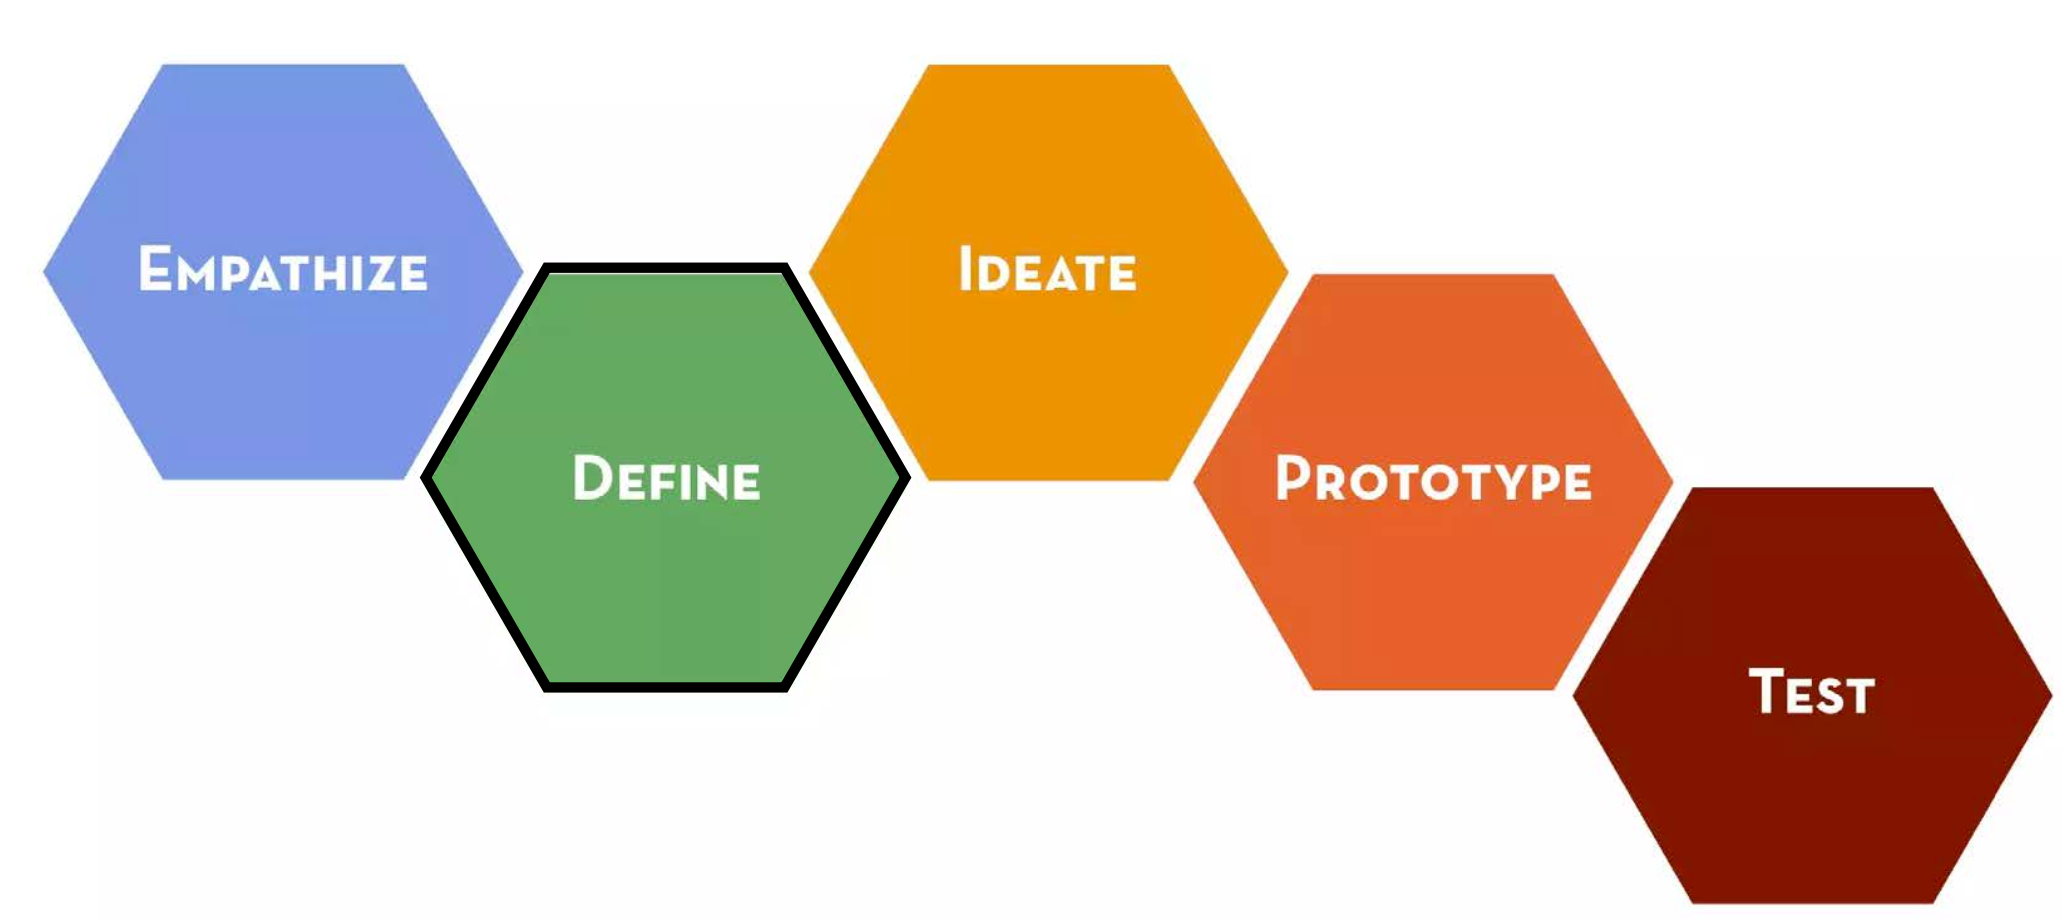
\includegraphics[width=\linewidth]{define.png}
\end{center}

\textbf{Define}
This part is more a focussing part and not flaring. Figure out what is important from collected data. Group info and find relations. \medskip

\textbf{Affinity Diagrams}

Data with affinity to each other are grouped together to form category. Groups are given labels, can be one or more categories in the end. 
Identify user, need and insight. Combined to create point of view. 

Good point of view insires the team, frames the problem in a focussed way. Empowers to make decisions and fiels brainstorming by suggesting "how might we" statements. \medskip

\textbf{The elastic user}
The elastic user can mean everyone and also noone. Vague and unfocused, lack of specifics makes it easy to rationalize any design. \medskip

\textbf{Personas}
Personas are precisely described. Act as stand-in for real users. Guide design decision. Fictitious but based on knowledge of real users. Informed from observations.
Personas are not elastic, don't make them fit the prototype. 

\begin{center}
	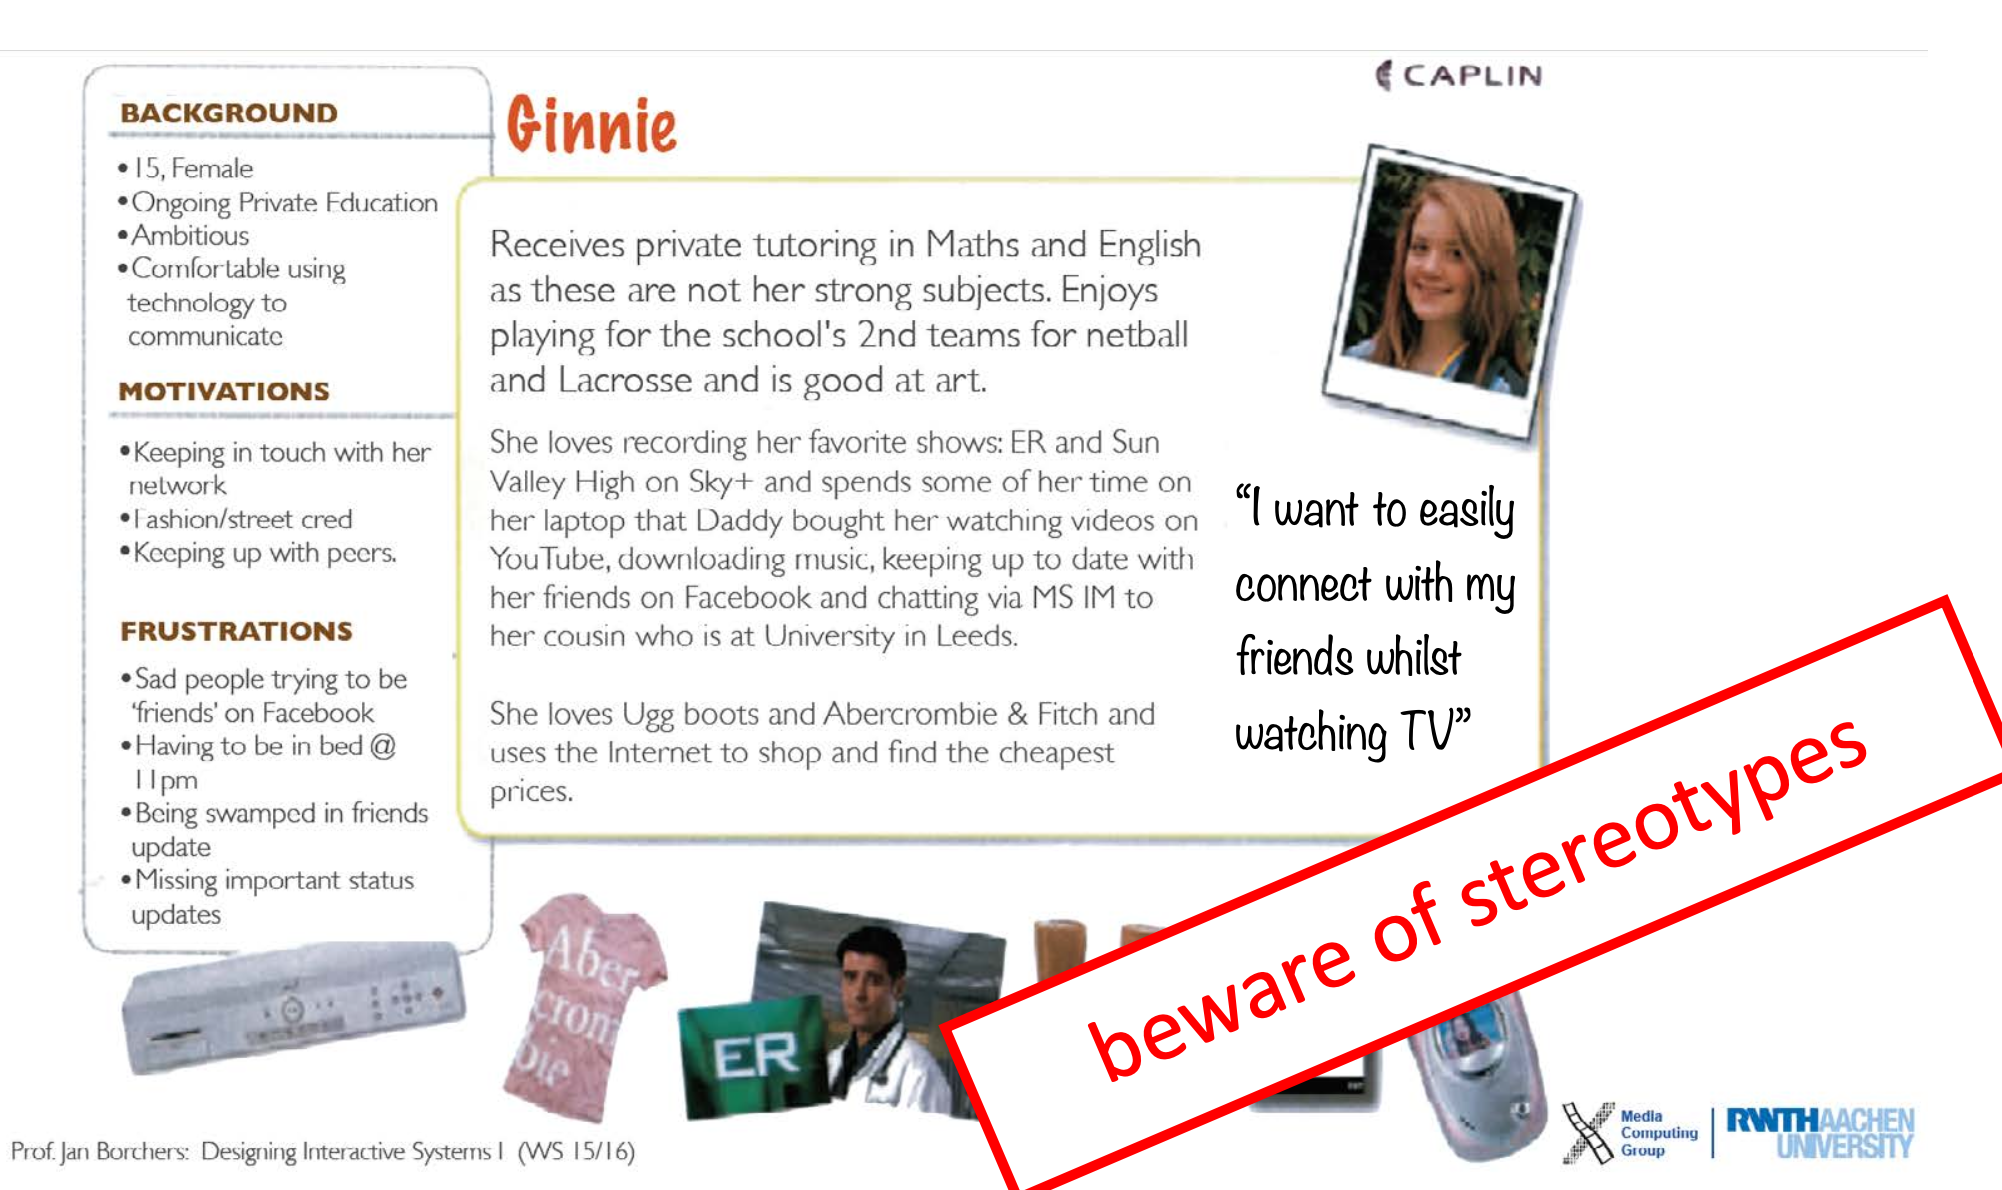
\includegraphics[width=\linewidth]{persona.png}
\end{center}

\begin{center}
	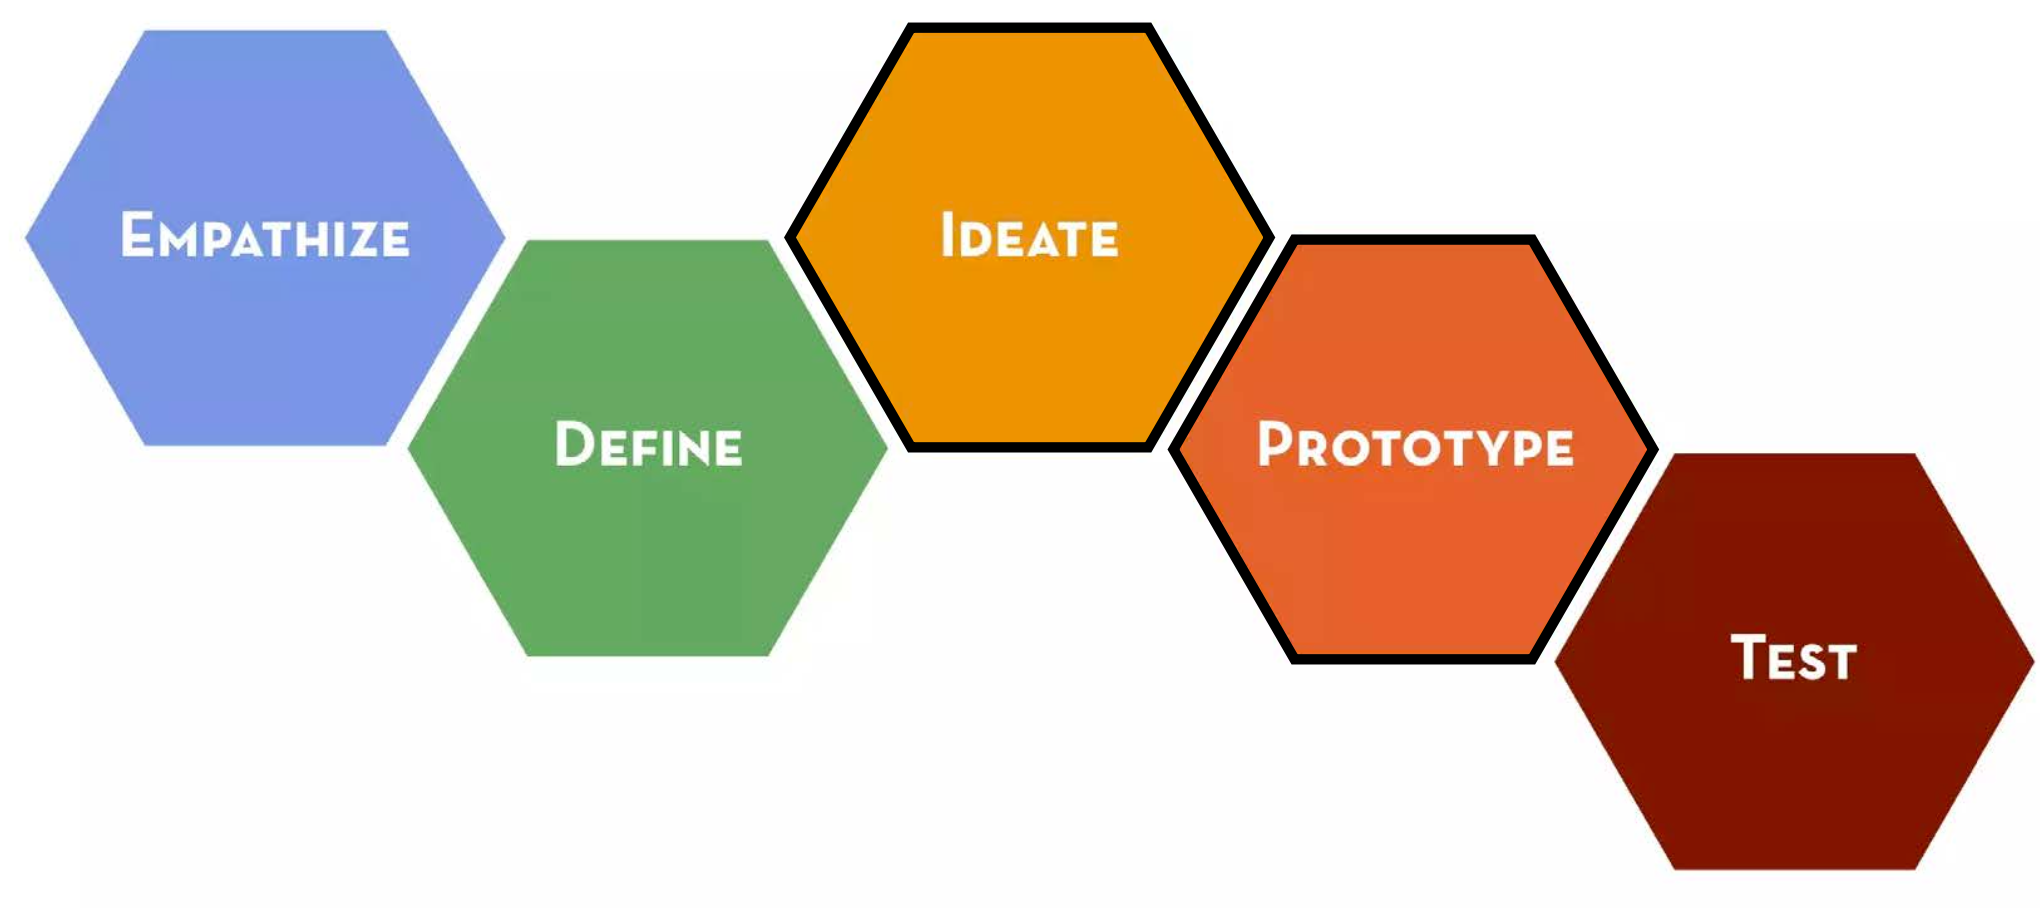
\includegraphics[width=\linewidth]{ideate.png}
\end{center}

\textbf{Ideate}
Flaring here, not focussing anymore. \medskip

\textbf{Ideation techniques}

\begin{multicols}{2}
    \begin{itemize}[itemsep=-5pt, topsep=-20pt, leftmargin=*]
	\item brainstorming
	\item mind-mapping
	\item storyboarding
	\item sketching
	\item low-fi prototyping
	\end{itemize}
\end{multicols}




\section{Prototyping}


Prototypes develop from sketches over time and are more defined in their criteria weights. 
Make multiple protopytes to evaluate different approaches and check for failure/success. Prototypes help us understand the requirements and specifications of the idea.
They answer a specific question. \medskip

\textit{Vertical vs. horizontal} \smallskip

Vertical provides critical path of one or few features (real feature on that path is completed, goes deep). Horizontal paths provide only overview with little to no functionality. \medskip

\textit{Fidelity and Interactivity}

\begin{center}
	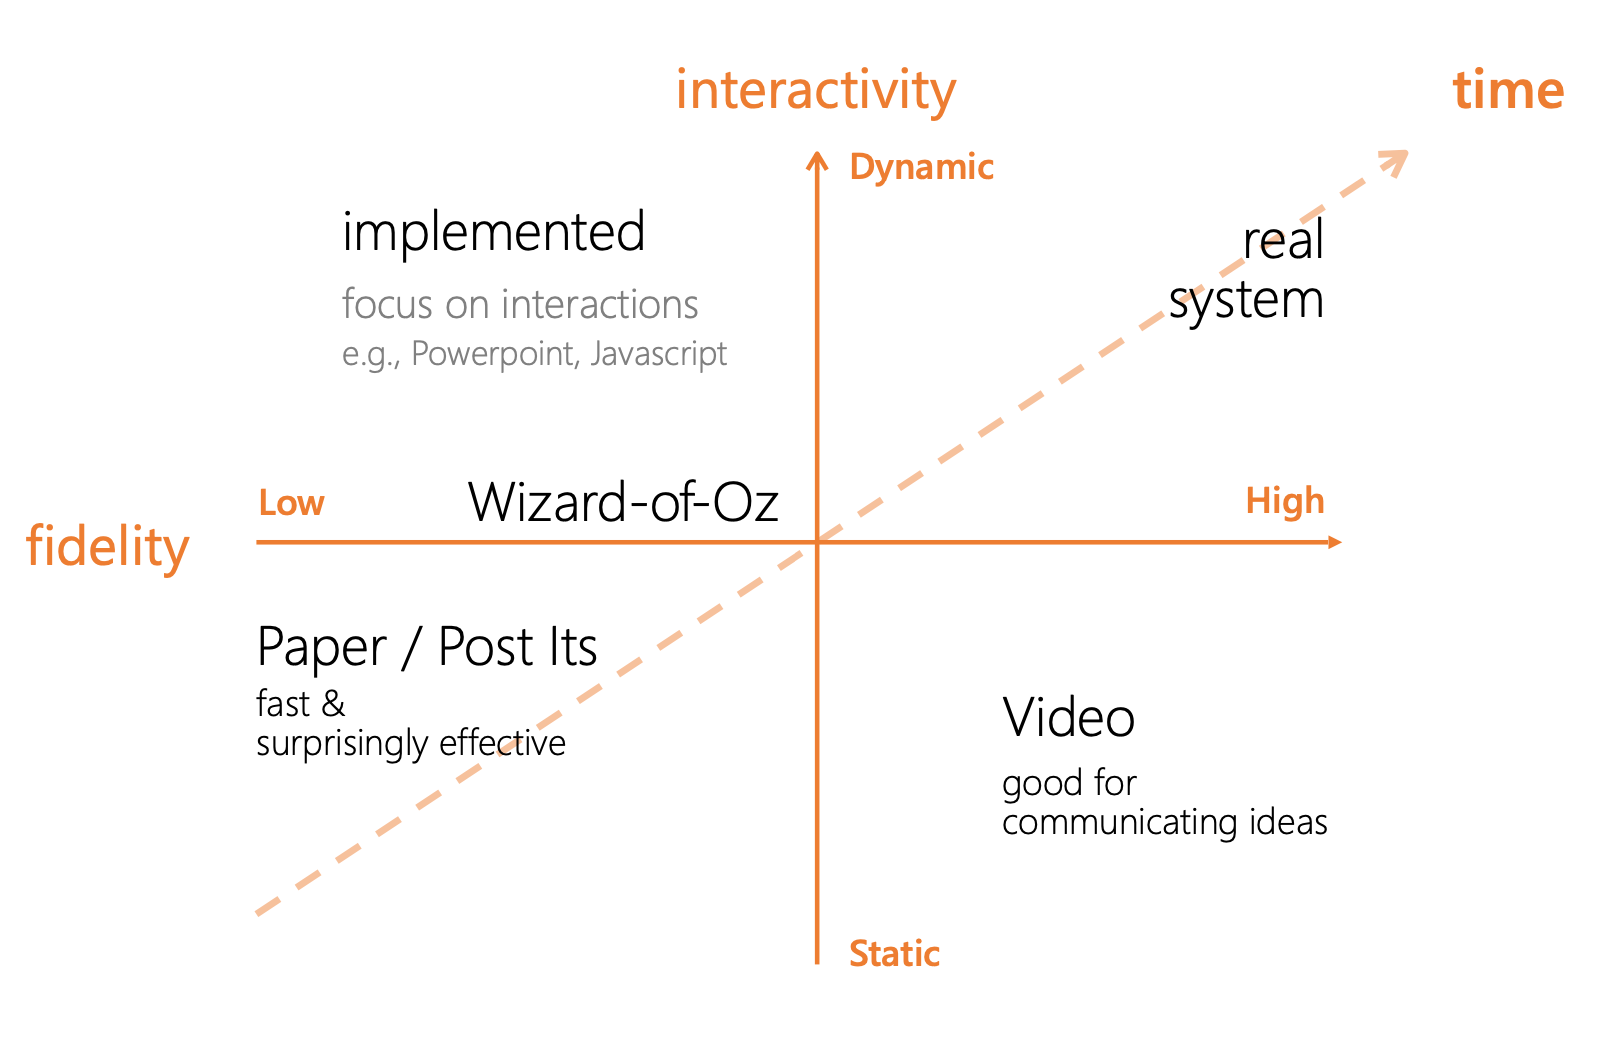
\includegraphics[width=\linewidth]{fidelity_iteractivity.png}
\end{center}


\textbf{Paper prototypes} \smallskip

Are rapid and cheap. \medskip

\textbf{Wizard of Oz} \smallskip

Interprets user input and simulated a system response. Allowes rapid testing of a complex feature before implementing. \medskip

\textbf{MidFi-Prototypes} \smallskip

Physical (paper, cardboard, lego etc.) to software. \medskip

\begin{multicols}{2}
    \begin{itemize}[itemsep=-5pt, topsep=-20pt, leftmargin=*]
	\item Powerpoint, Keynote
	\item AdobeXD, Figma
	\end{itemize}
\end{multicols}



\begin{center}
	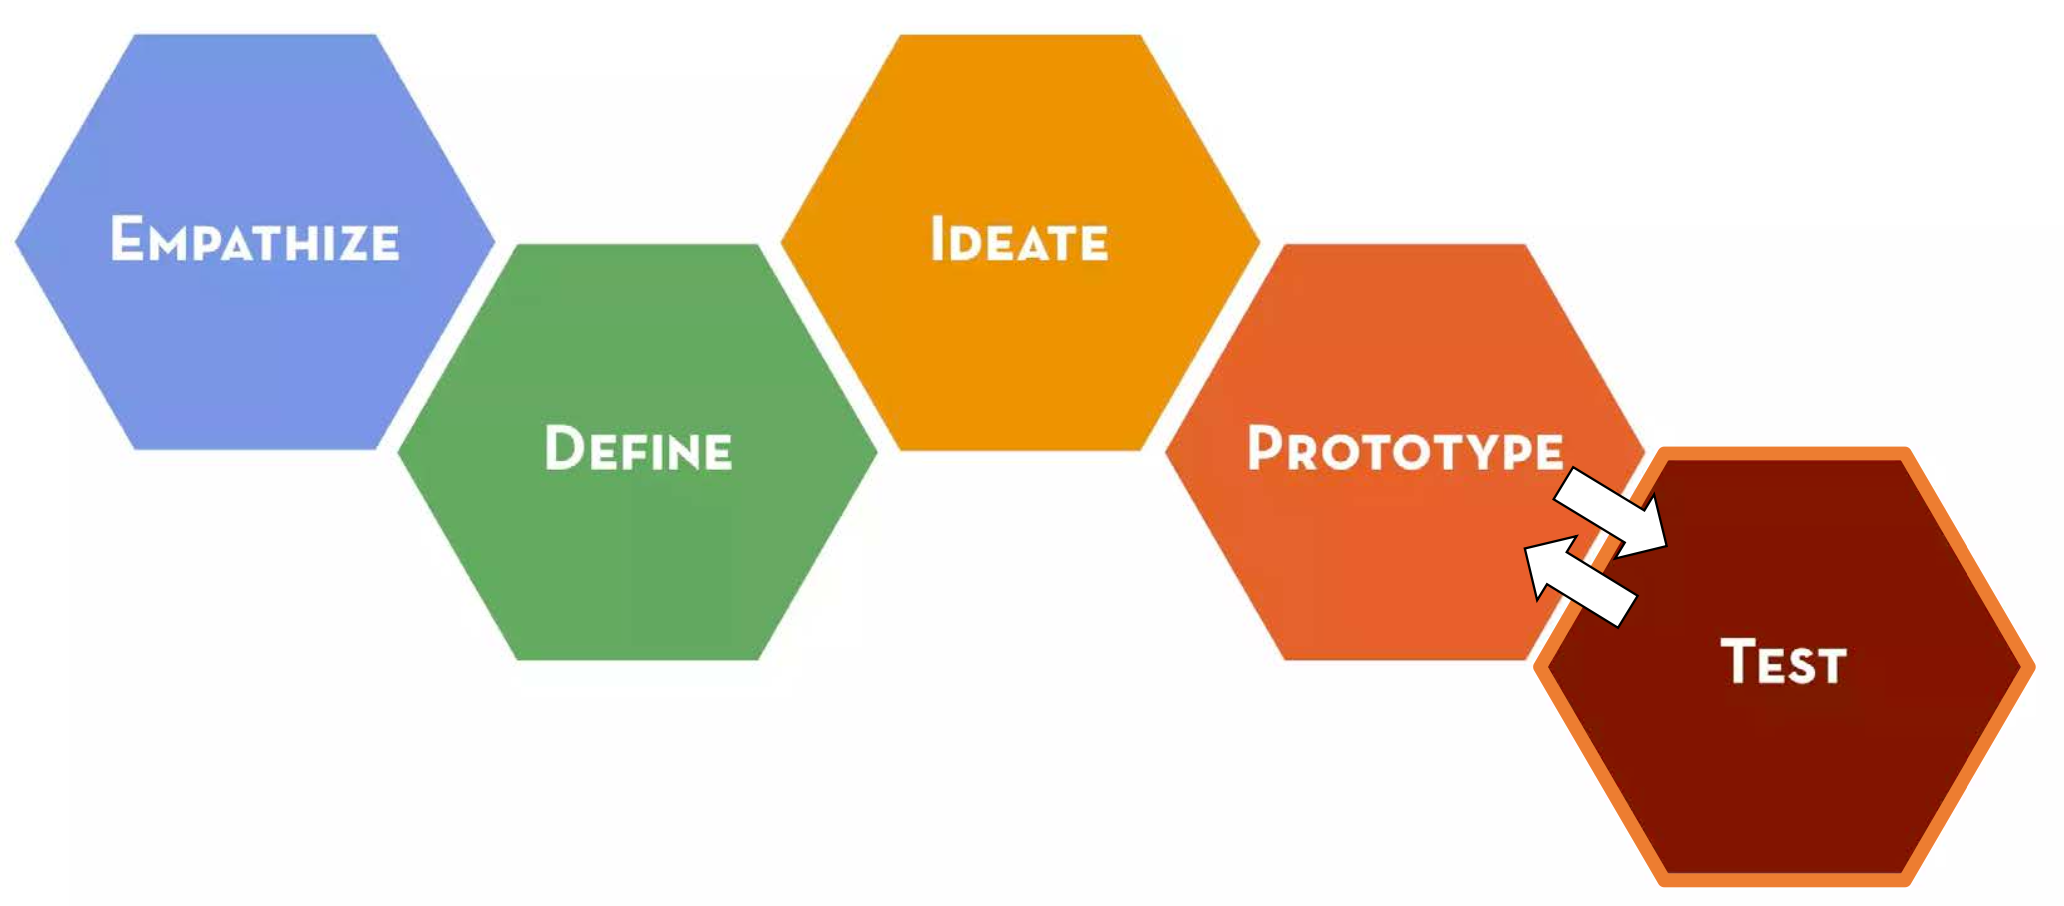
\includegraphics[width=\linewidth]{prototype_test.png}
\end{center}


\textbf{Analytical vs. Empirical} \smallskip

\textit{Analytical} \smallskip

Look at inherent attributes of the design, rather then the design in use. Intrinsic characteristics of the design. 
Examples are usability/UX inspection methods, design walkthroughs, heuristic evaluations. \medskip

\textit{Empirical} \smallskip

Based on how well a design or design change pays off in terms of real observable usage. Includes quantitative and qualitative data. 
Examples are usability/UX scores, controlled experiments and case studies. \medskip

\textbf{Formative vs. Sumative} \smallskip

\textit{Formative} \smallskip

Helps form the design. Part of iterative process. Evaluations done during testing. Mainly collects qualitative data but also quantitative. Focusses on what is not working.\smallskip

\textit{Summative} \smallskip

Helps sum up the design. Evaluates the success of the finished product, and compares with competitors. Collects quantitative data, and focussed mainly on what is working. \medskip


\textbf{Evaluation criteria for UI design} \smallskip

\textit{Usability} \smallskip

Extent to which product can be used by specific users to achieve goals with effectiveness, efficiency and satisfaction.
\smallskip
Five quality components of Usability:

\begin{multicols}{2}
    \begin{itemize}[itemsep=-5pt, topsep=-20pt, leftmargin=*]
	\item learnability
	\item efficiency
	\item memorability
	\item errors
	\item satisfaction
	\end{itemize}
\end{multicols}

\columnbreak

\textit{User Experience} \smallskip

Totality of the effect(s) felt by a user as a result of interaction with the usage context of a system. device or product. 

It includes:  
\begin{multicols}{2}
    \begin{itemize}[itemsep=-5pt, topsep=-20pt, leftmargin=*]
	\item Usability
	\item Usefulness
	\item Emotional impact
	\item Savoring memory after interaction
	\end{itemize}
\end{multicols}
It embraces seeing, touching, thinking about the system or product and admiring it and its presentation.
Focusses on holistic experience of the user. \medskip


\textbf{Affordances} \smallskip 

Actions that the design of an object suggests to the user. Provide strong clues to how objects are to be used without labels, explanations or manuals.
Works for both physical objects and software. Up to a certain degree of complexity. 

\section{Analytical Investigation}

\begin{center}
	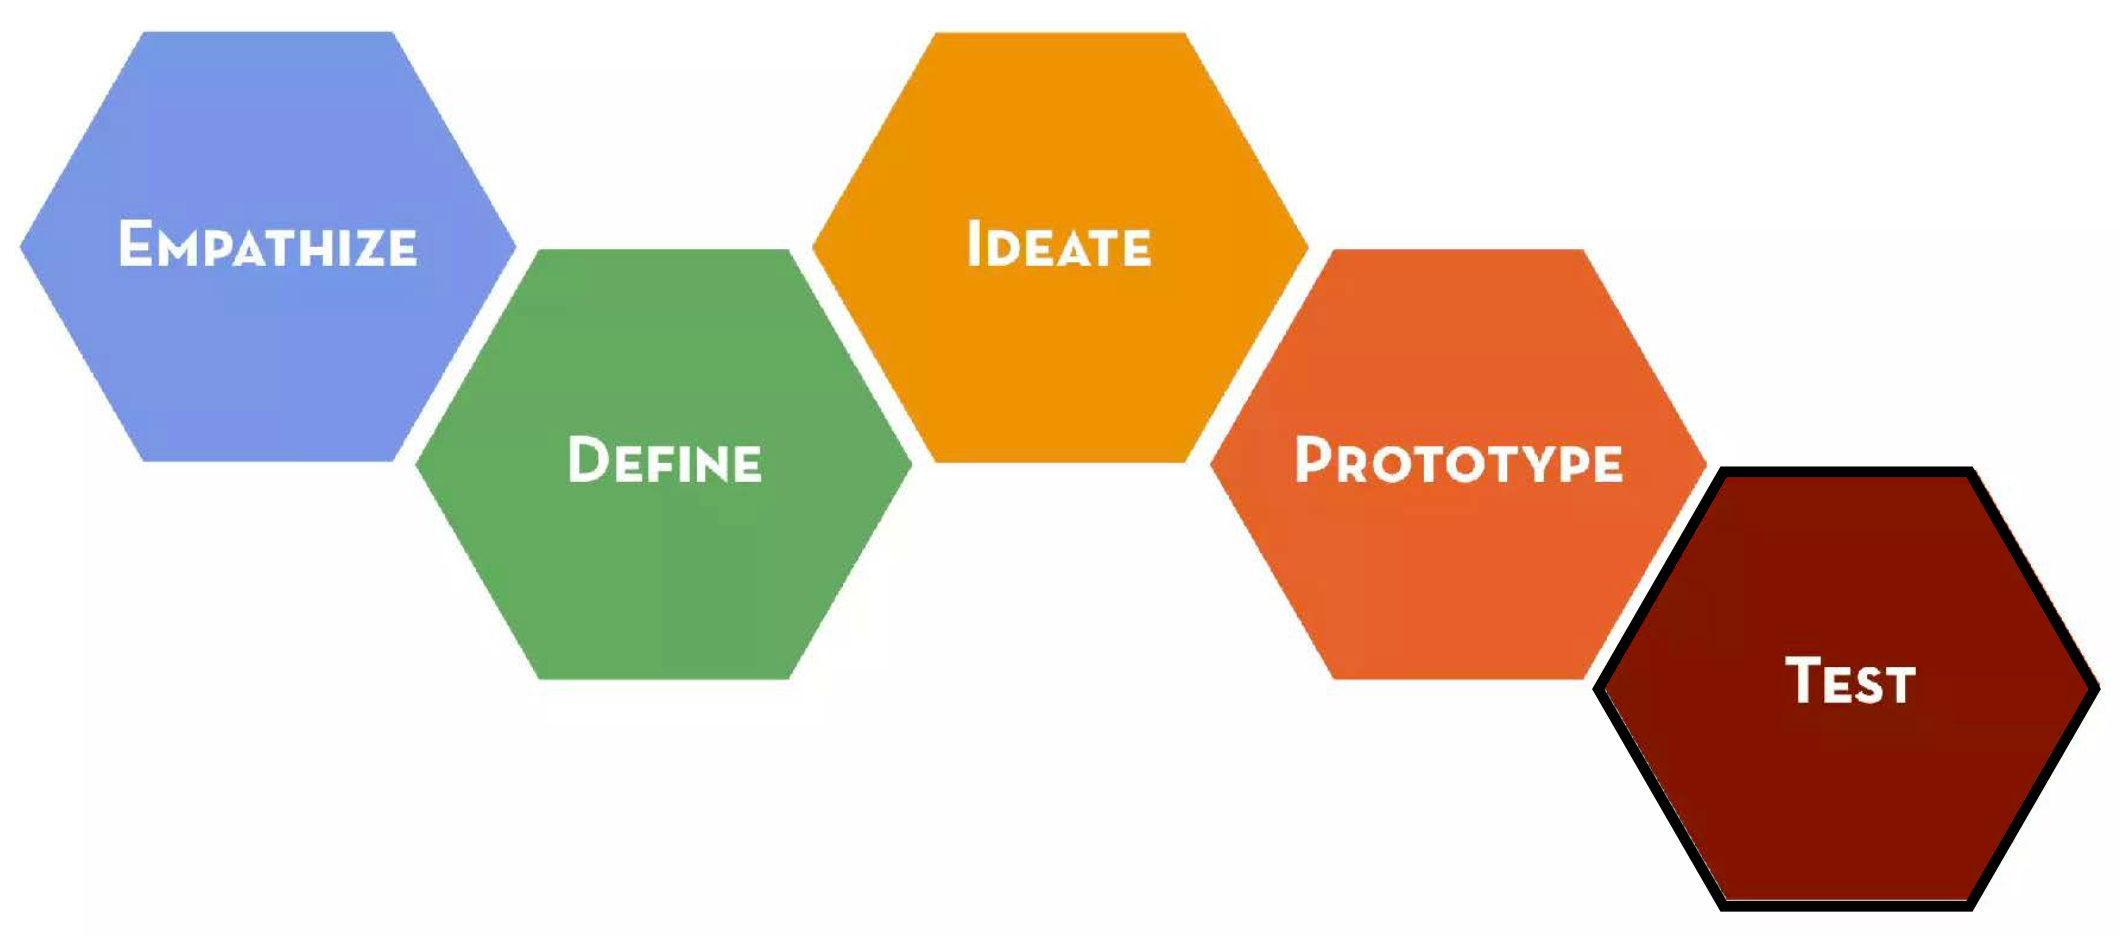
\includegraphics[width=\linewidth]{test.png}
\end{center}

Is performed by usability experts and domain experts. They use their knowledge of users and technology to assess the usability and user experience. Result can be formal or informal reports. 

Two types of analytical investigation: 

\begin{enumerate}
    \item Usability and UX inspection (Design, cognitive walktrhoughs, heuristic evaluation)
    \item Predictive user performance models (GOMS, KLM)
\end{enumerate}

\medskip

\textbf{1. Usability and UX inspection} \smallskip

\textit{Cognitive Walkthroughs} \smallskip

Evaluate design by experts, with the goal of exploring the design on behalf of the users.
Difference to UX inspection: Ux inspection only one aspect of a design presented to experts. Cognitive walkthrough: More focussed on ease-of-learning.  \medskip

\textit{Heuristic Evaluation} \smallskip

Heuristics are design guidelines. 
Examine the interface, judge is compliance with recognized usability principles (heuristics).
Is cheap, fast and easy to use. Is developed for inexperiences practicioners, experts can be limited through heuristics. Can be done on paper-only prototypes. \smallskip


\begin{enumerate}
    \item Briefing to tell evaluators what to do
    \item Each evaluator inspects interface alone (at least twice, get feel for flow of interaction and scope of system, also focus on specific interface elements)
    \item evaluators aggregate findings
    \item debriefing session, discussion of possible redesigns for major UX problems, look as positive aspects
\end{enumerate}

Optimally between 3 and 5 evaluators. Limited because it does not encourage to take a rich and comprehensive view of interaction. Its only a rough outline, and expert find problems withs inspection not heuristics. 
Danger of overestimating heuristics and use for any evaluation. \medskip

\textbf{Nielsen's Heuristics} \smallskip


\textit{1. Visibility of system status} \smallskip

System should always keep users informed about what is going on, through approp. feedback in reasonable time. \medskip

\textit{2. Match between system and the real world} \smallskip

System should speak the users' language, wih words, phrases and concepts familiar to the user, rathen thans system-oriented terms. Follow real world conventions, make info appear in natural and logical order. \medskip

\textit{3. User control and freedom} \smallskip

Users need a clearly marked emergency exit from unwanted state, if chosen system functions by mistake. \medskip

\textit{4. Consistency and standards} \smallskip

User should not have to wonder whether different words, situations or actions mean the same thing. \medskip

\textit{5. Error prevention} \smallskip

Good error messages, but better is design that prevents a proble  from occurring in the first place. Eliminate error-prone conditions or check for them and give users a confirmation option before commiting to the action. \medskip

\textit{6. Recognition rather than recall} \smallskip

Minimize the user's memory load by making opjects, options and actions visible. Instructions for use of the system should be visible or easily retrievable, whenever appropriate. \medskip

\textit{7. Flexibility and efficiency of use} \smallskip

Accelerators may often speed up the interaction for the expert user, such that the system can support both inexperienced and experienced users. \medskip

\textit{8. Asthetic ans minimalist design} \smallskip

Dialogs should not contain irrelevant or rarely needed information. Extra infos compete with the relevant units of information. \medskip


\textit{9. Help users recognize, diagnose and recover from errors} \smallskip

Error messages should be expressed in plain language, precisely indicate the problem and constructively suggest a solution.

\textit{10. Help and documentation} \smallskip

Even it is better if the system can be used without documentation, it may be necessary to provide help and documentation. Should be easy to reach, list concrete steps and should not be too extensive. \medskip


\textbf{2. Predictive User performance models} \smallskip

Way of evaluating roducts or design without directly involving users. Estimated of efficiency of systems for different tasks. \smallskip

We use GOMS to model knowledge about the system and cognitive provesses involved when users interact with systems. 

We use KLM to provide numerical predictions to performance and estimate chains of operations. \medskip

\textbf{GOMS model} \smallskip

\textit{Goals} \smallskip

The state the user wants to achieve. \medskip

\textit{Operators} \smallskip

Cognitive processes and pyhsical actions needed to attain the coals (mouse click etc.) \medskip

\textit{Methods} \smallskip

Procedures for accomplishing th goals, drage mouse over search gield, type in term, press go etc ... \medskip

\textit{Selection Rules} \smallskip

Decide which method to select when there is more than one. \smallskip

Goms example:
\begin{center}
	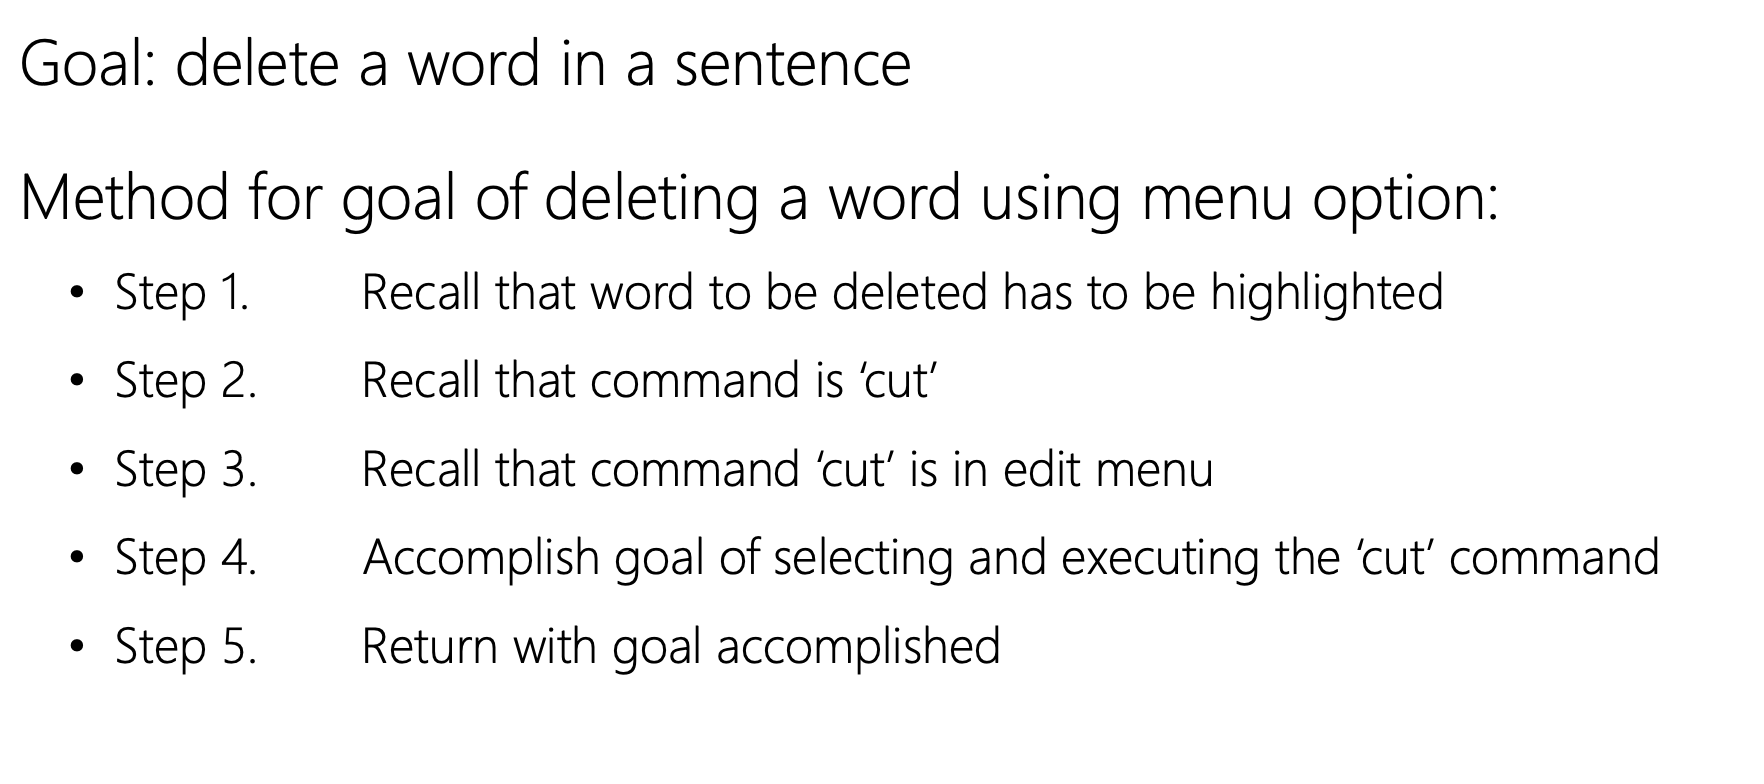
\includegraphics[width=\linewidth]{goms_example.png}
\end{center}

\textbf{Keystroke Level model (KLM)} \smallskip

Mesarues and compares execution times. 

\begin{center}
	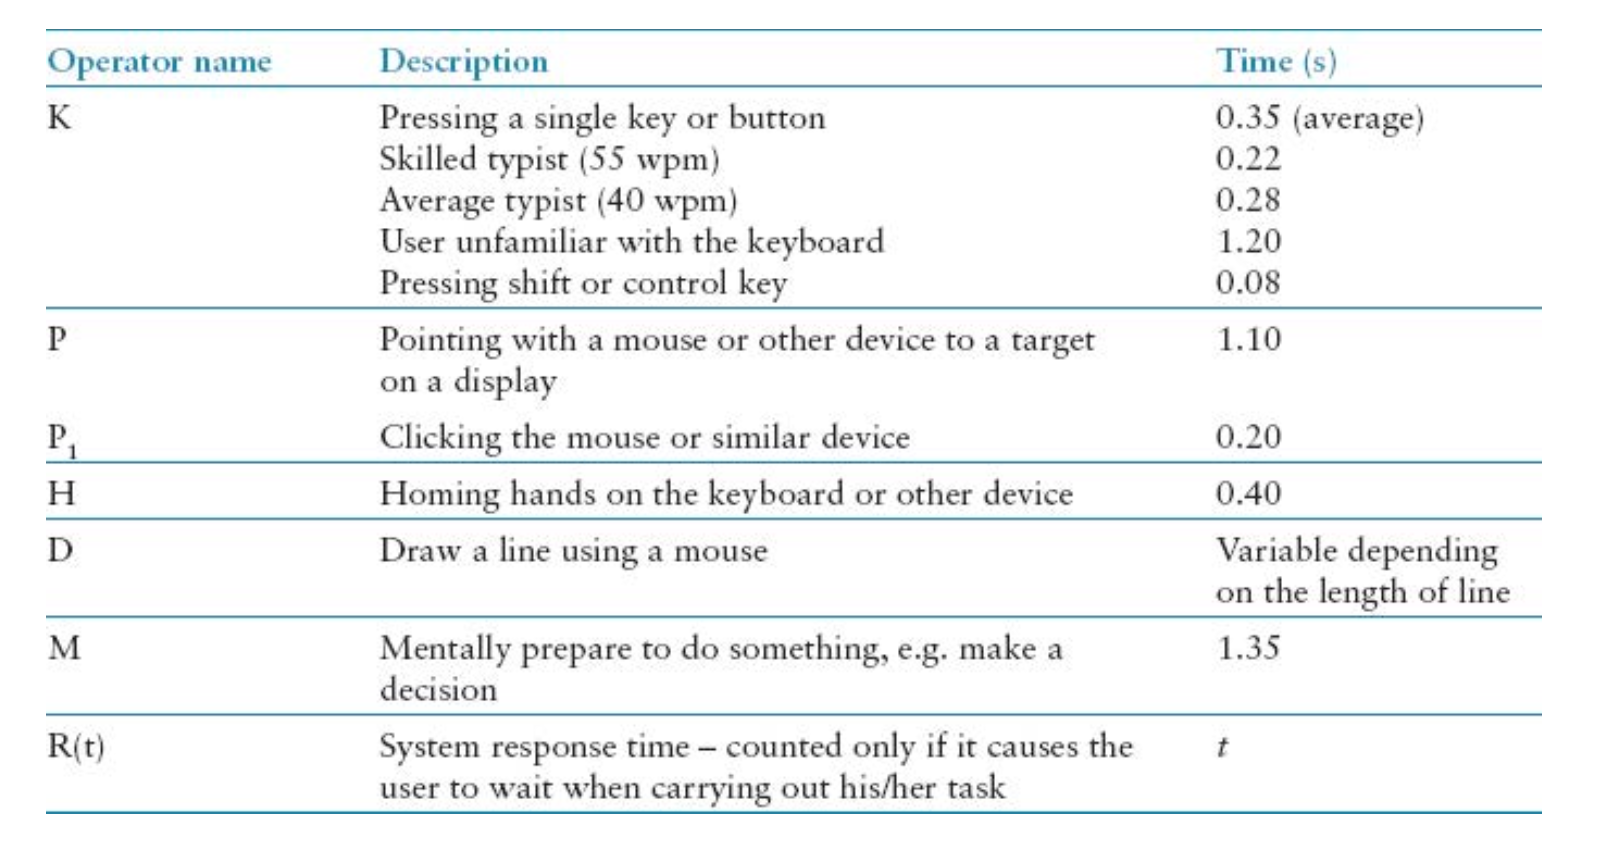
\includegraphics[width=\linewidth]{klm_model.png}
\end{center}


\textit{Predictive models strengths and weaknesses} \medskip


\begin{itemize}
    \item Relatively to perform comaprative analysis for different interfaces and prototypes, specifications. 
    \item Can only model high-level tasks, involving small set of high routine low level tasks
    \item Only valid for predictable/expert behavior (no multi-tasking, fatigue, learning effects etc)
\end{itemize}





\section{Evaluations and Experimental Design}

\textit{Formative} early in the design process, sanity checks that we're building the right thing. \textit{Summative} to check if we improved upon our last iteration, does it work better than other solutions? \medskip

\textbf{Quantitative Evaluation Methods}

Ensure certain level of quality, comparesolutions objectively, attain a scientific statement. \medskip

\textbf{Primary Usability Metrics} \smallskip

\begin{center}
	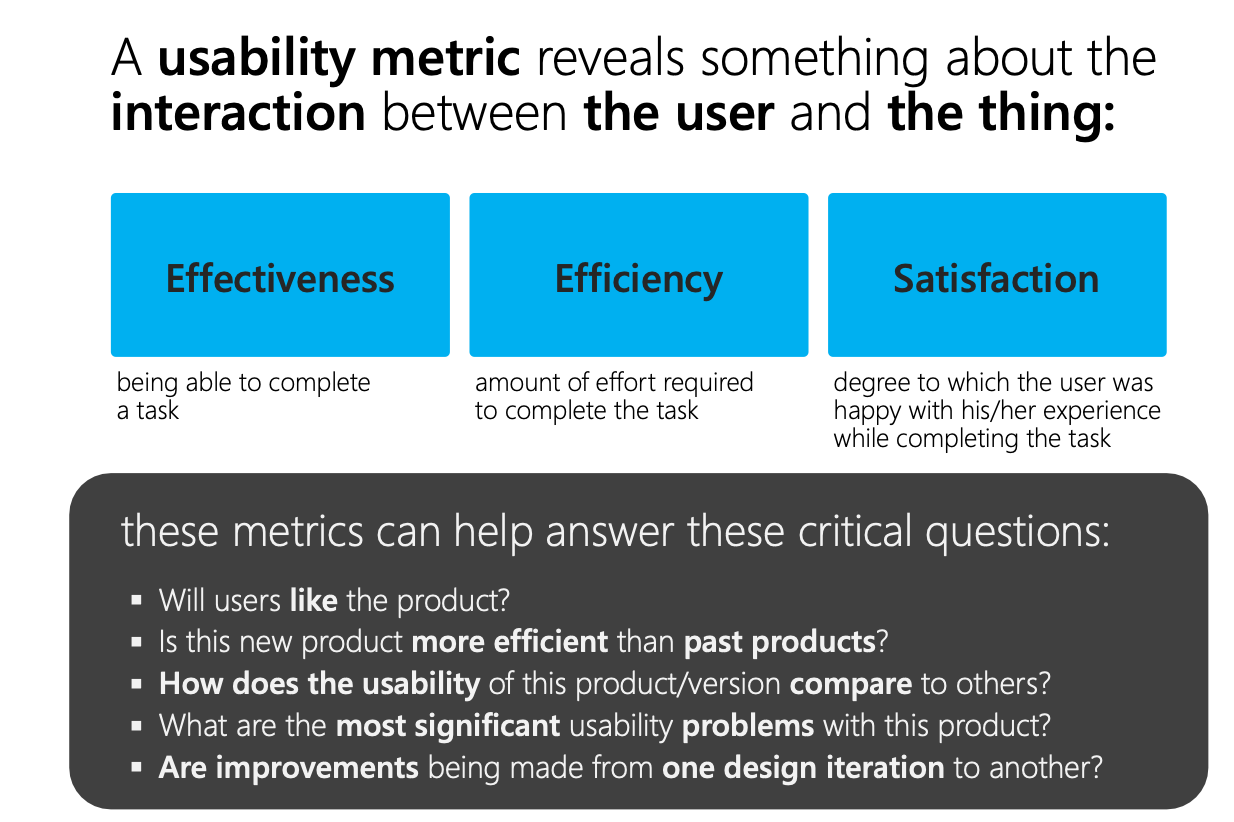
\includegraphics[width=\linewidth]{metrics.png}
\end{center}

\textbf{Cause and Effect} \smallskip

We want to identify clear causal links. Cause precedes effect, they need to correlate and other explanations have to be ruled out. 
Isolate causality by controlled experiments. Alter design with suspected cause absent (control) and present (experimental condition).
All other conditions should be identical. \medskip

\textbf{Quasiexperimentell | Observational} \smallskip

We observe that independent variable and dependent variable are highly correlated, but did not control for anything (for instance participation in exercices and final exam grade). \medskip

\textbf{Experimental | Controlled} \smallskip

We randomly assign students to exercise and no exercise condition, then we controlled for other variables and results implies causality. \medskip


\textbf{characteristics of Emprical Methods}

\begin{itemize}
    \item Objectivity
    \item Reproducibility
    \item Validity (internally and externally)
    \item Relevance
\end{itemize}

For instance threat to external validity is over-use of specific participant groups (only psychology or cs students). \medskip

\textbf{The experiment}

Indepdendent variables affect the dependent (measured) variables through experiment.

Variables can be catagorical, ordinal (ordered discrete), or cardinal/interval (continuous) data. \medskip

\textbf{Designing an empirical study}

\begin{enumerate}
    \item What is being compared? (which Indepdendent variables)
    \item What are they bing comapred in? (dependent variables, metrics)
    \item What lse is being varied? (extraneous variables to control/eliminate)
    \item Relevance
\end{enumerate}

Look at slide set 5 for various examples. \medskip

\textbf{More complex comparisons}

Different experimental designs possible: \textit{Within subjects:} Everyone-does everything. \textit{Between subjects:} Only on condition per group. \medskip

\textbf{Latin Square Counterbalancing}

\begin{center}
	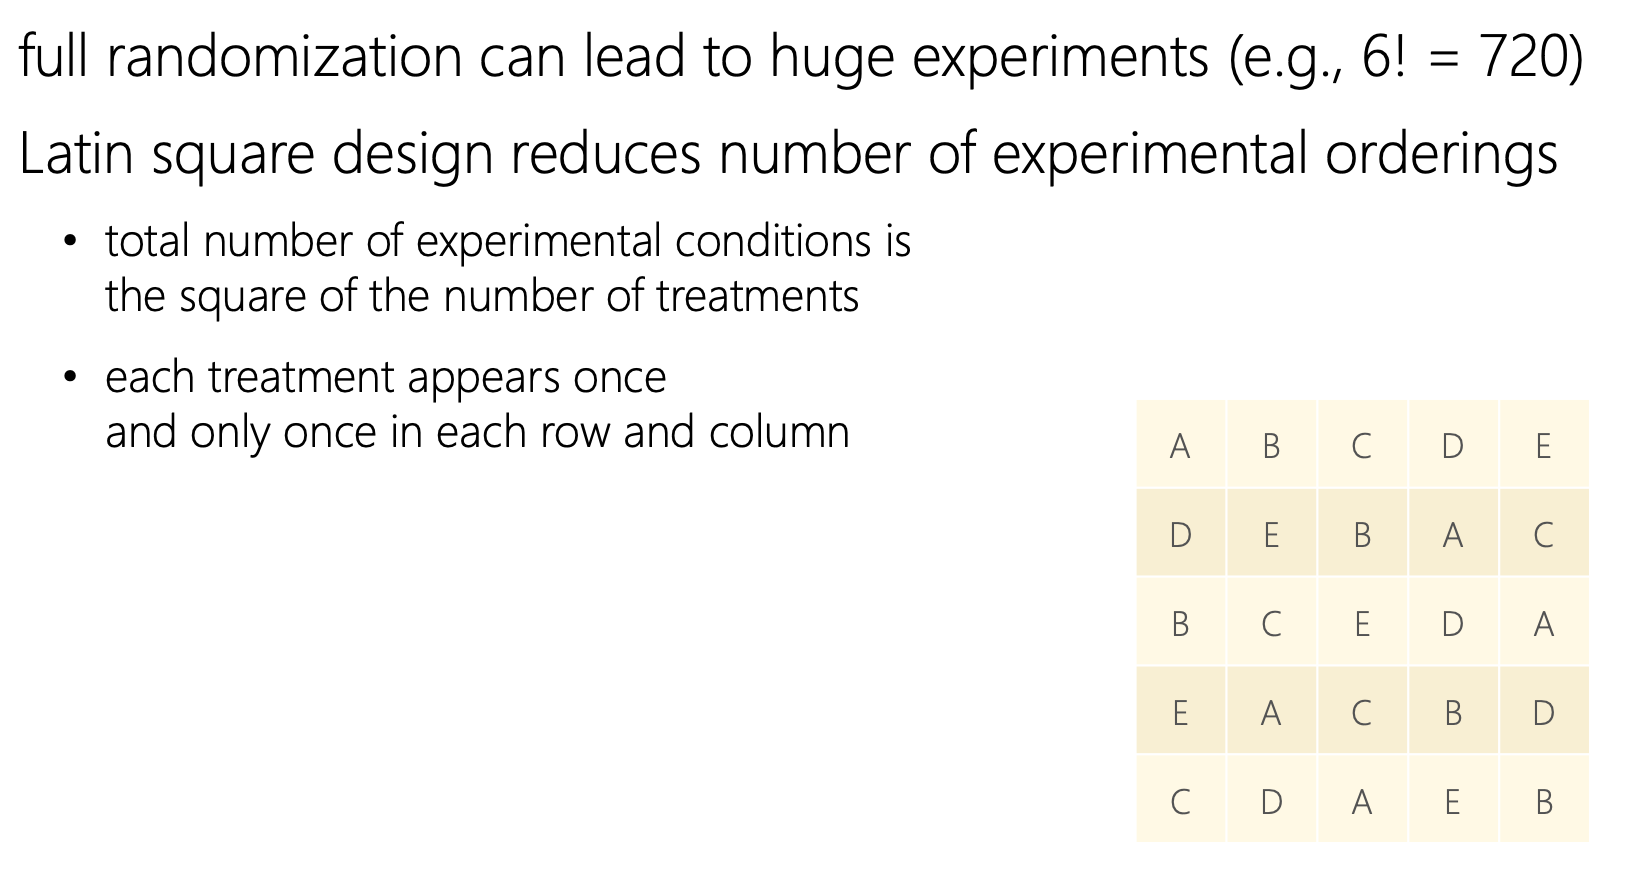
\includegraphics[width=\linewidth]{latin_square.png}
\end{center}


\textbf{Latin Square Example for 5}

\begin{center}
	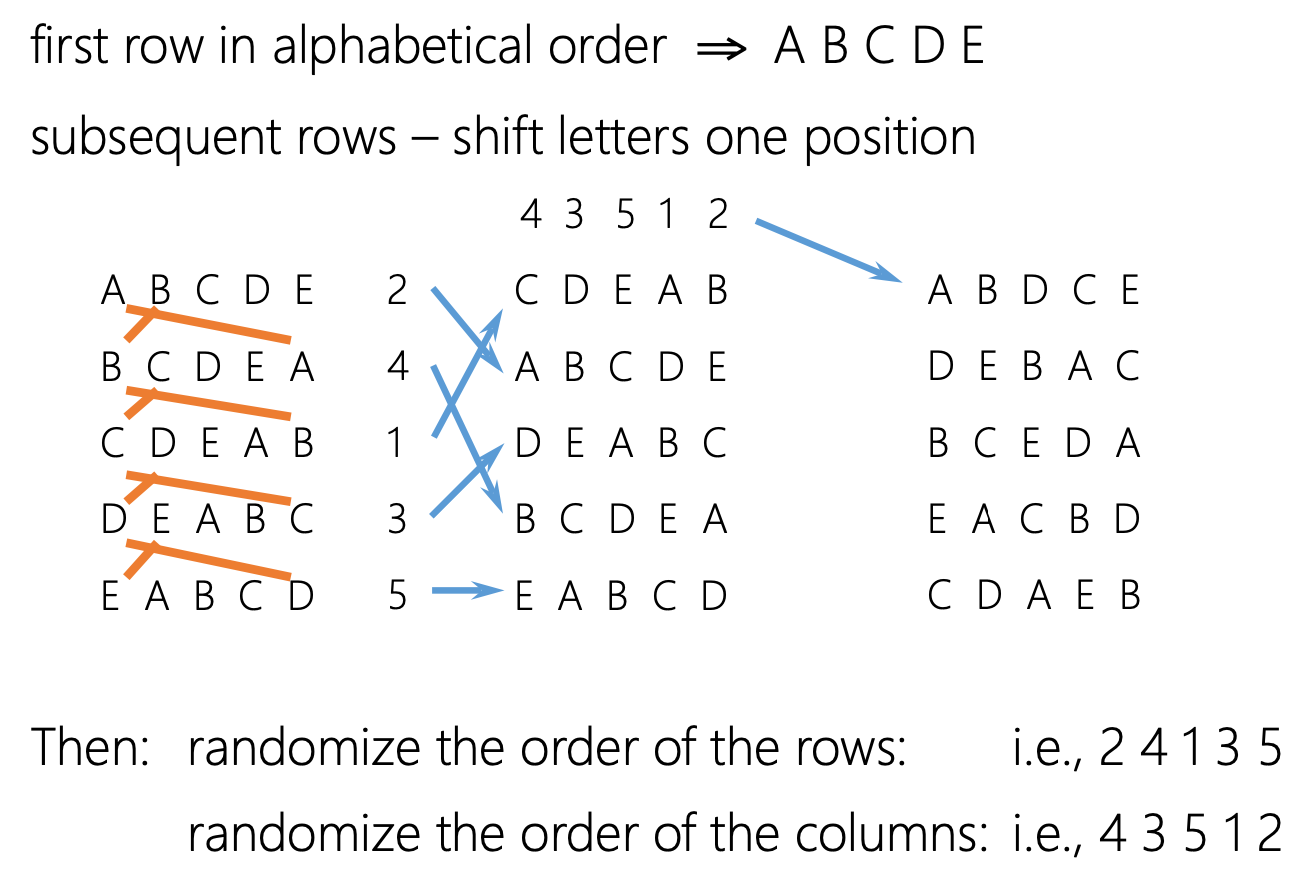
\includegraphics[width=\linewidth]{latin_example.png}
\end{center}

\section{Statistical Analysis}

\textbf{Data Collection}

\textit{Population vs Sample}


\begin{center}
	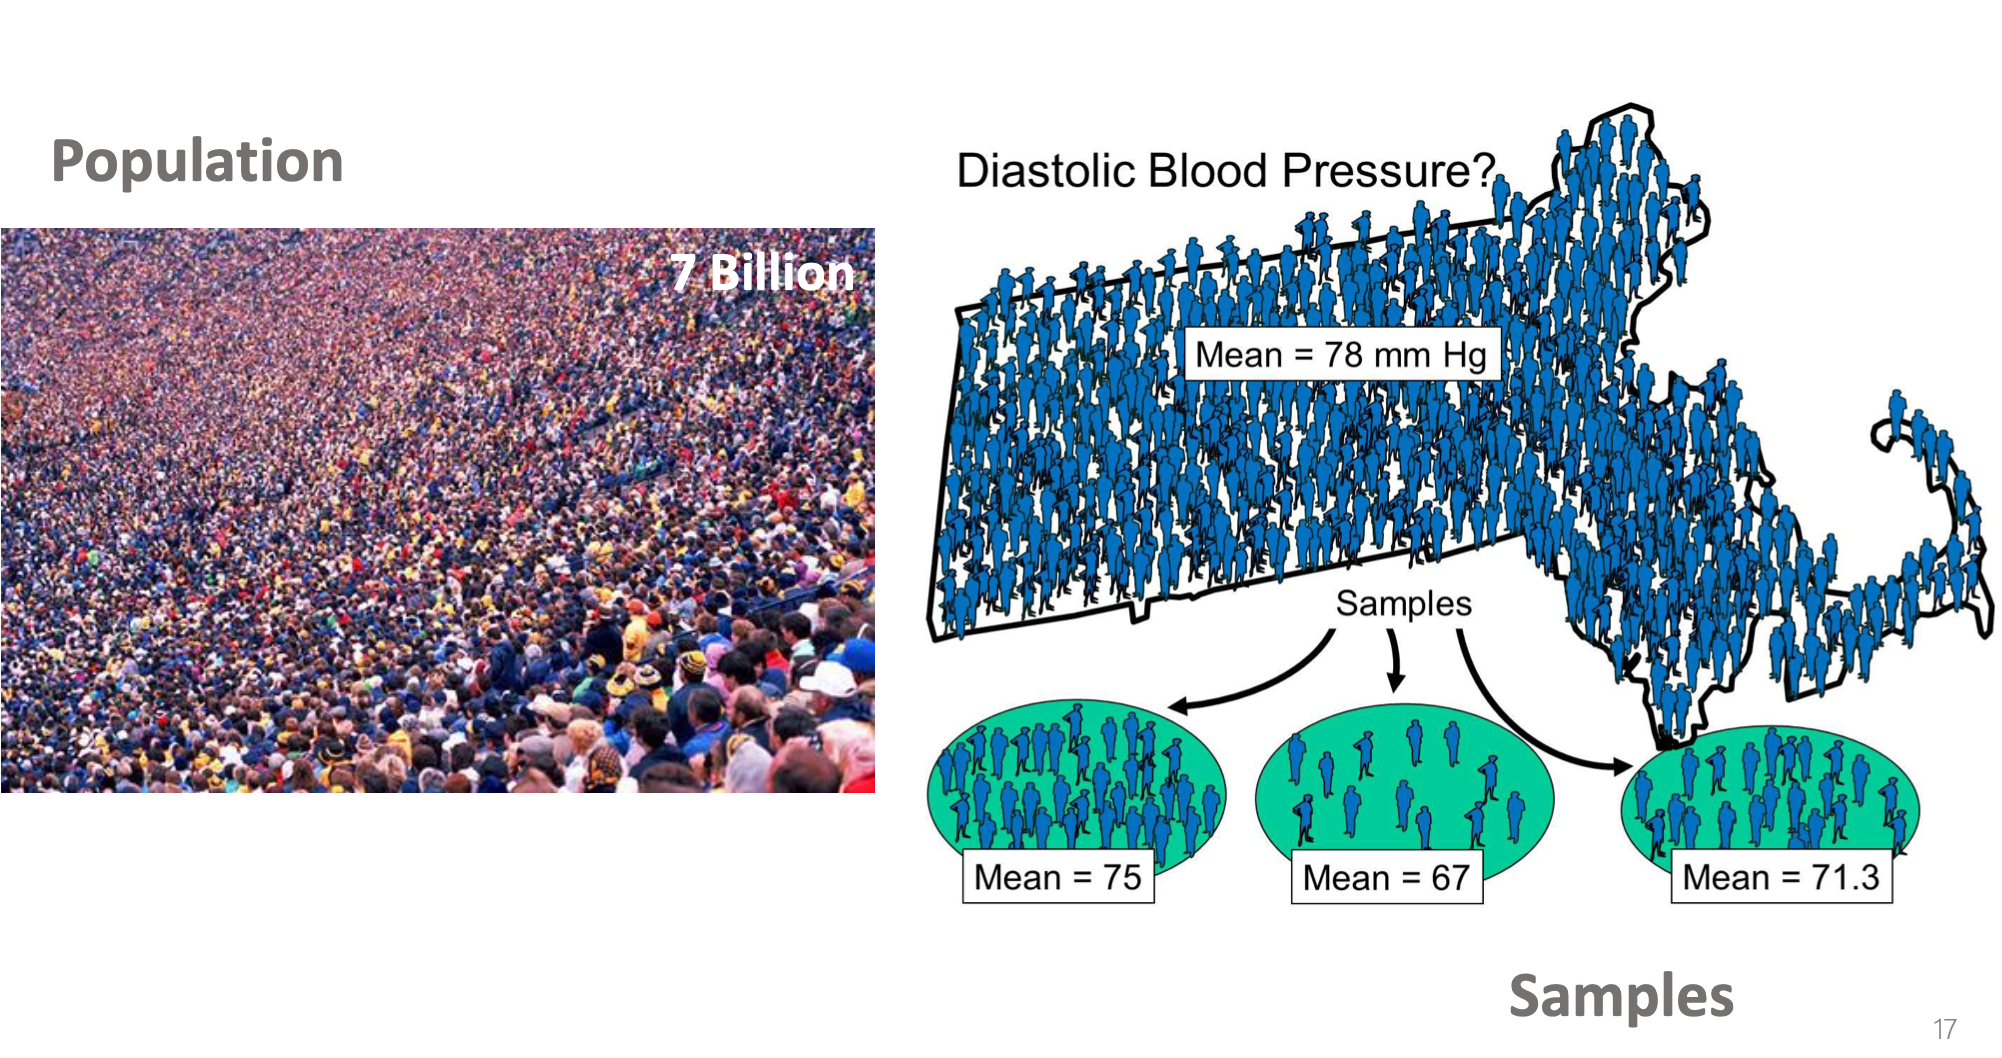
\includegraphics[width=\linewidth]{population_sample.png}
\end{center}


\textit{Generalizability}


\textit{Hypothesis testing}


\textbf{Descriptive statistics and validation}

\textit{Mean}

\textit{Median}


\textit{Distribution}

\textit{Confidence Interval (CI)}


\textbf{Analysis}

\textit{Frequentist Approaches}


\textit{Hypothesis testing}

\textit{P-Value}

\textit{Alpha-Level}

\textit{Errors}

\textit{Degrees of Freedom}


\textit{Independent vs dependent samples}


\textit{Parametrix vs. non-parametric tests}


\textit{A/B Testing}


\textit{Indepdendent t-test}


\textit{From t-value to significance}


\textit{ANOVA analysis of Variance}


\textit{Effect size}

\textit{Powere analysis}


\textit{Software for statistical analysis}


\textbf{Reporting}


\textit{Writing up the results}
















\section{User Modeling}

\textbf{Human vs Computer}

\textit{Strengths of human} \smallskip

\begin{itemize}[itemsep=-5pt, topsep=0pt, leftmargin=*]
    \item intuition
    \item memorize cohesive information
    \item signal detection under noise
    \item recognizing complex signals (speech etc.)
    \item recognizing complex configurations (scenes etc.)
    \item adaption to unexpected situations
    \item learning aptitude
\end{itemize}

\medskip


\textit{Strengths of computer} \smallskip

\begin{itemize}[itemsep=-5pt, topsep=0pt, leftmargin=*]
    \item measuring and counting
    \item storing large amounts of incoherent data
    \item detecting known signals
    \item fast and reliable reaction to signals
    \item reliable fatigue free reaction to known signals
    \item superiority if problems can be algorithmically formulated
\end{itemize}

\medskip

\textbf{Model Human Processor} \smallskip


We can look at humans as an information processor. Taking the computers output as input and after processing outputting processed information as input for the computer. \smallskip

The humans perception, memory and motor system can be applied to estimate execution time, error rates, training effects for simple stimulation /reaction interactions and system parameters. \smallskip

\begin{center}
	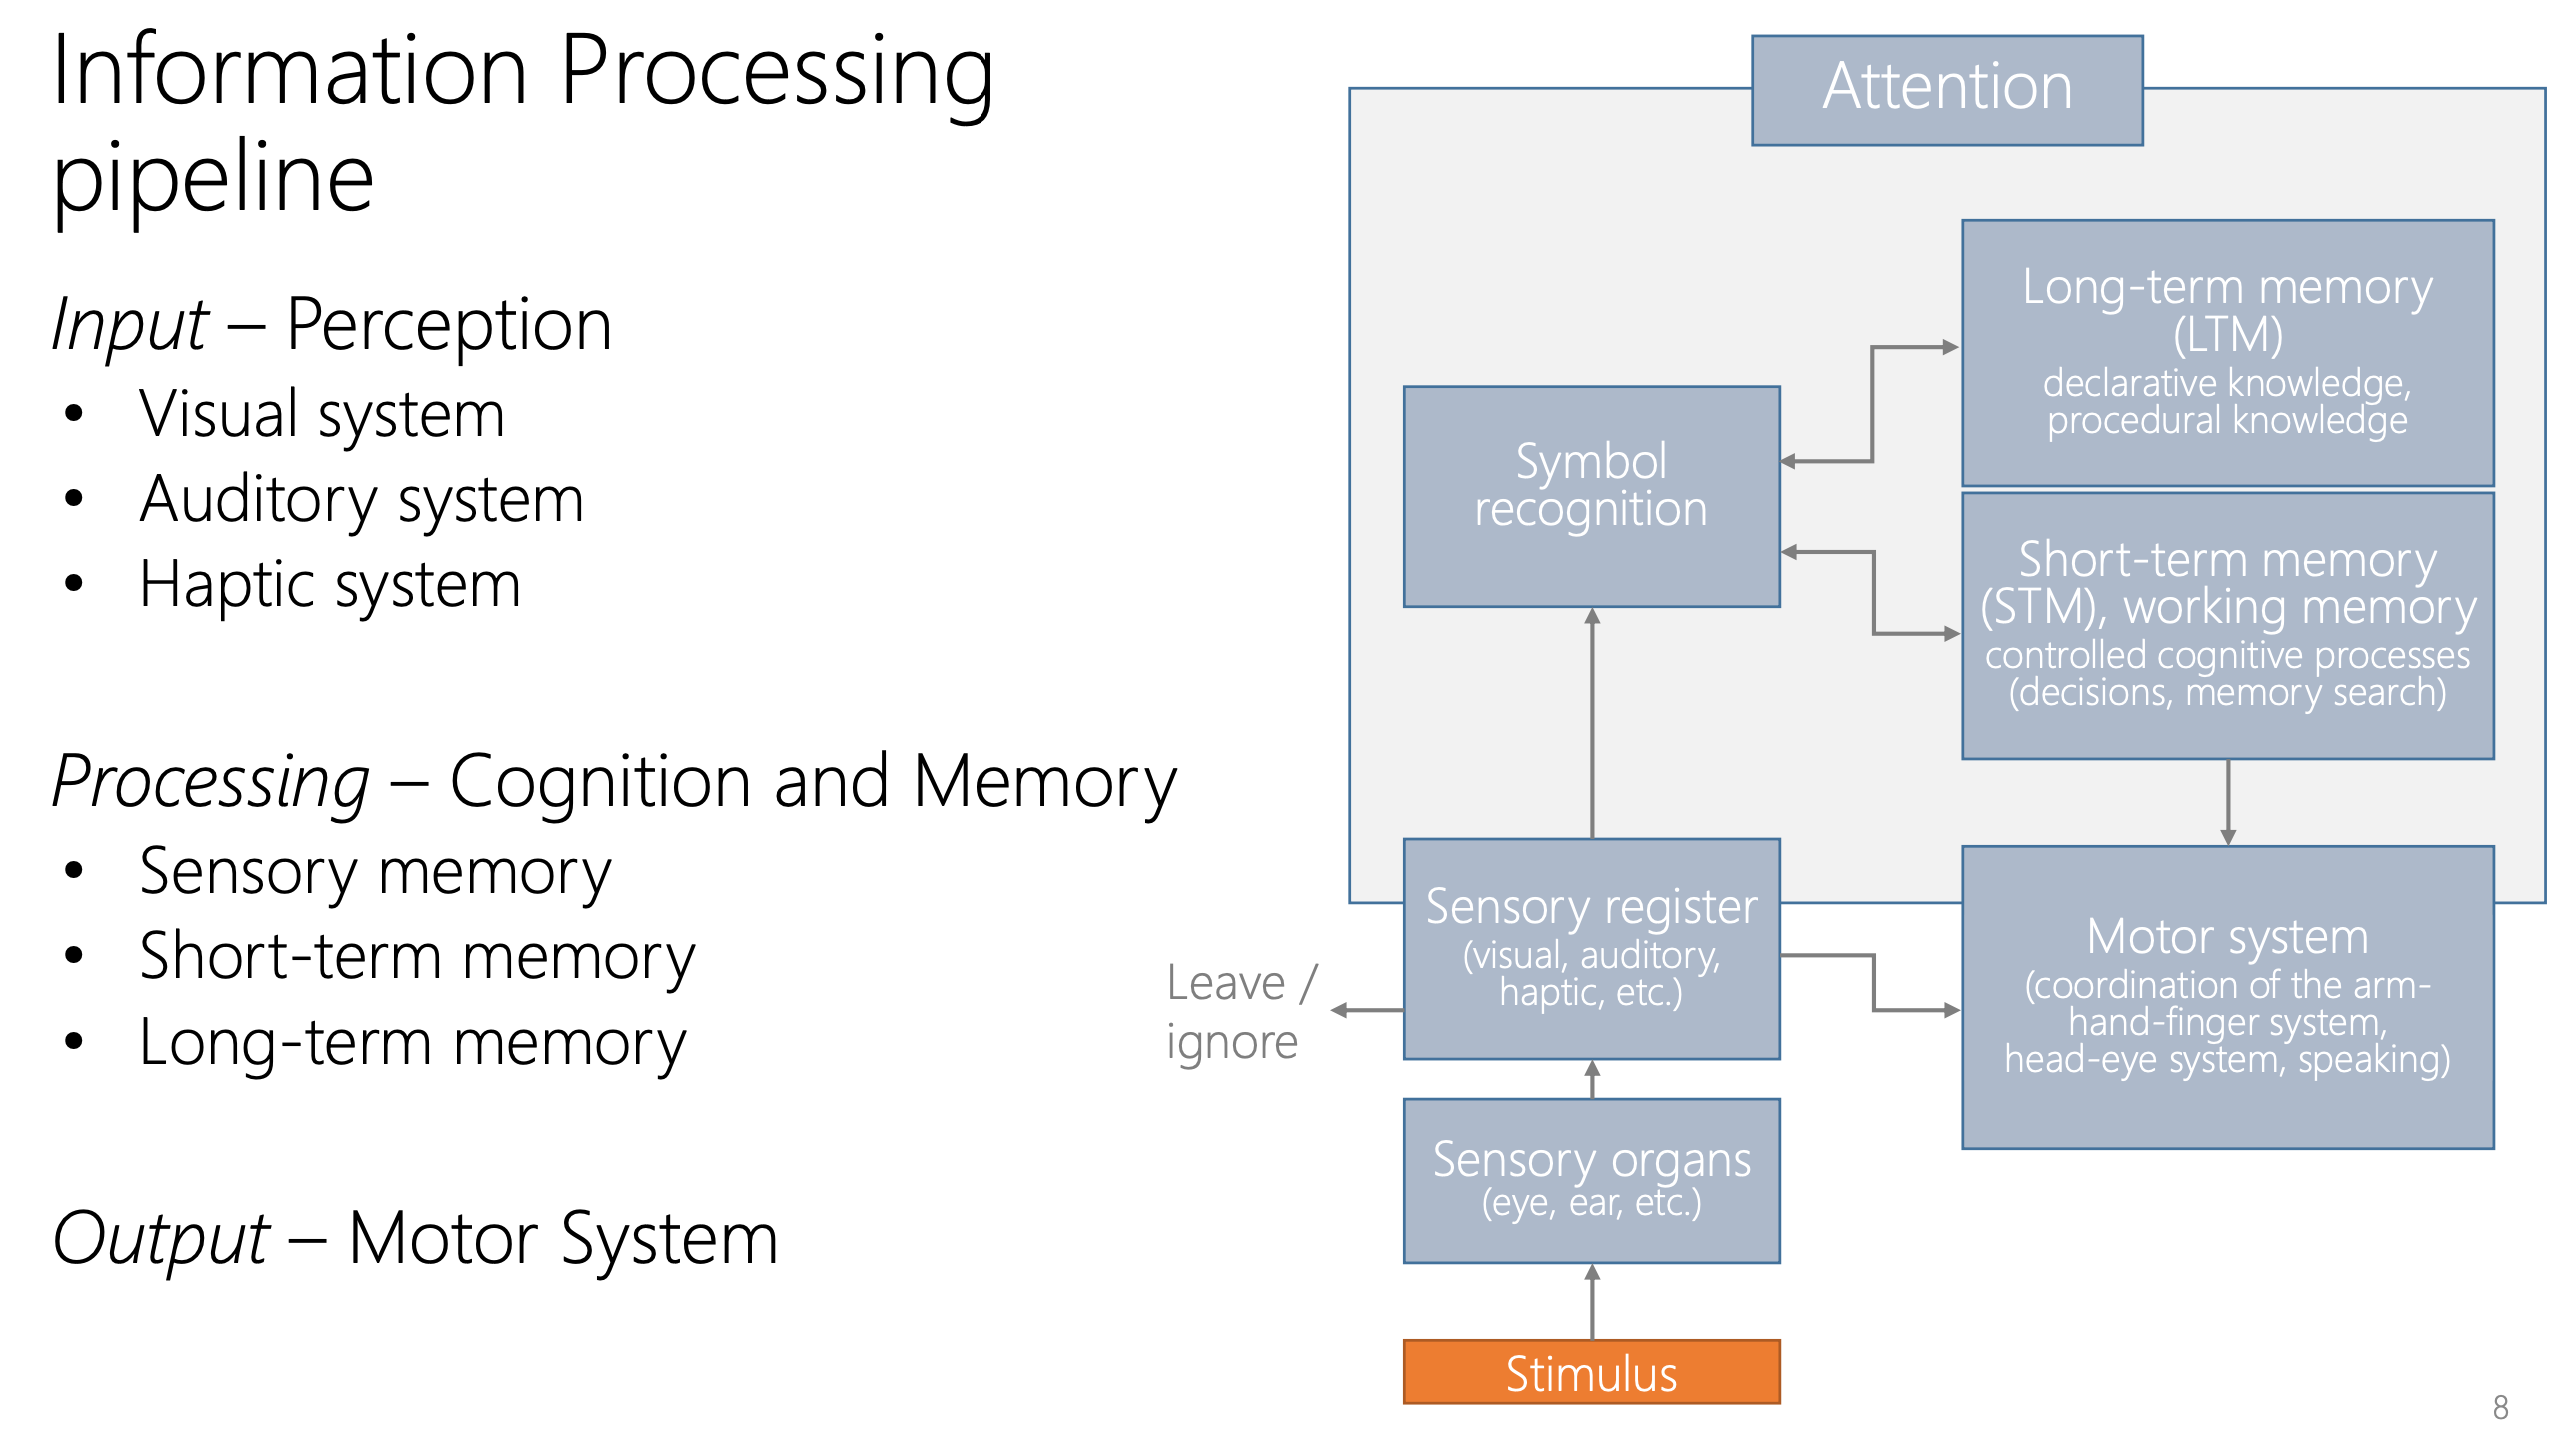
\includegraphics[width=\linewidth]{information_processing.png}
\end{center}


\columnbreak

We look at three main processors with associated memory: \smallskip

\textit{Perceptual System} \smallskip

Containing sensors and buffers. \medskip

\textit{Cognitive System} \smallskip

Containing working memory and content symbolically coded \medskip

\textit{Motor System} \smallskip

Contains movements. \medskip

Each processor has associated runtime. Overall runtime is sum of them.  \medskip

\textbf{Perception (Visual System)}


\textit{Anatomy of human eye} \smallskip


\begin{center}
	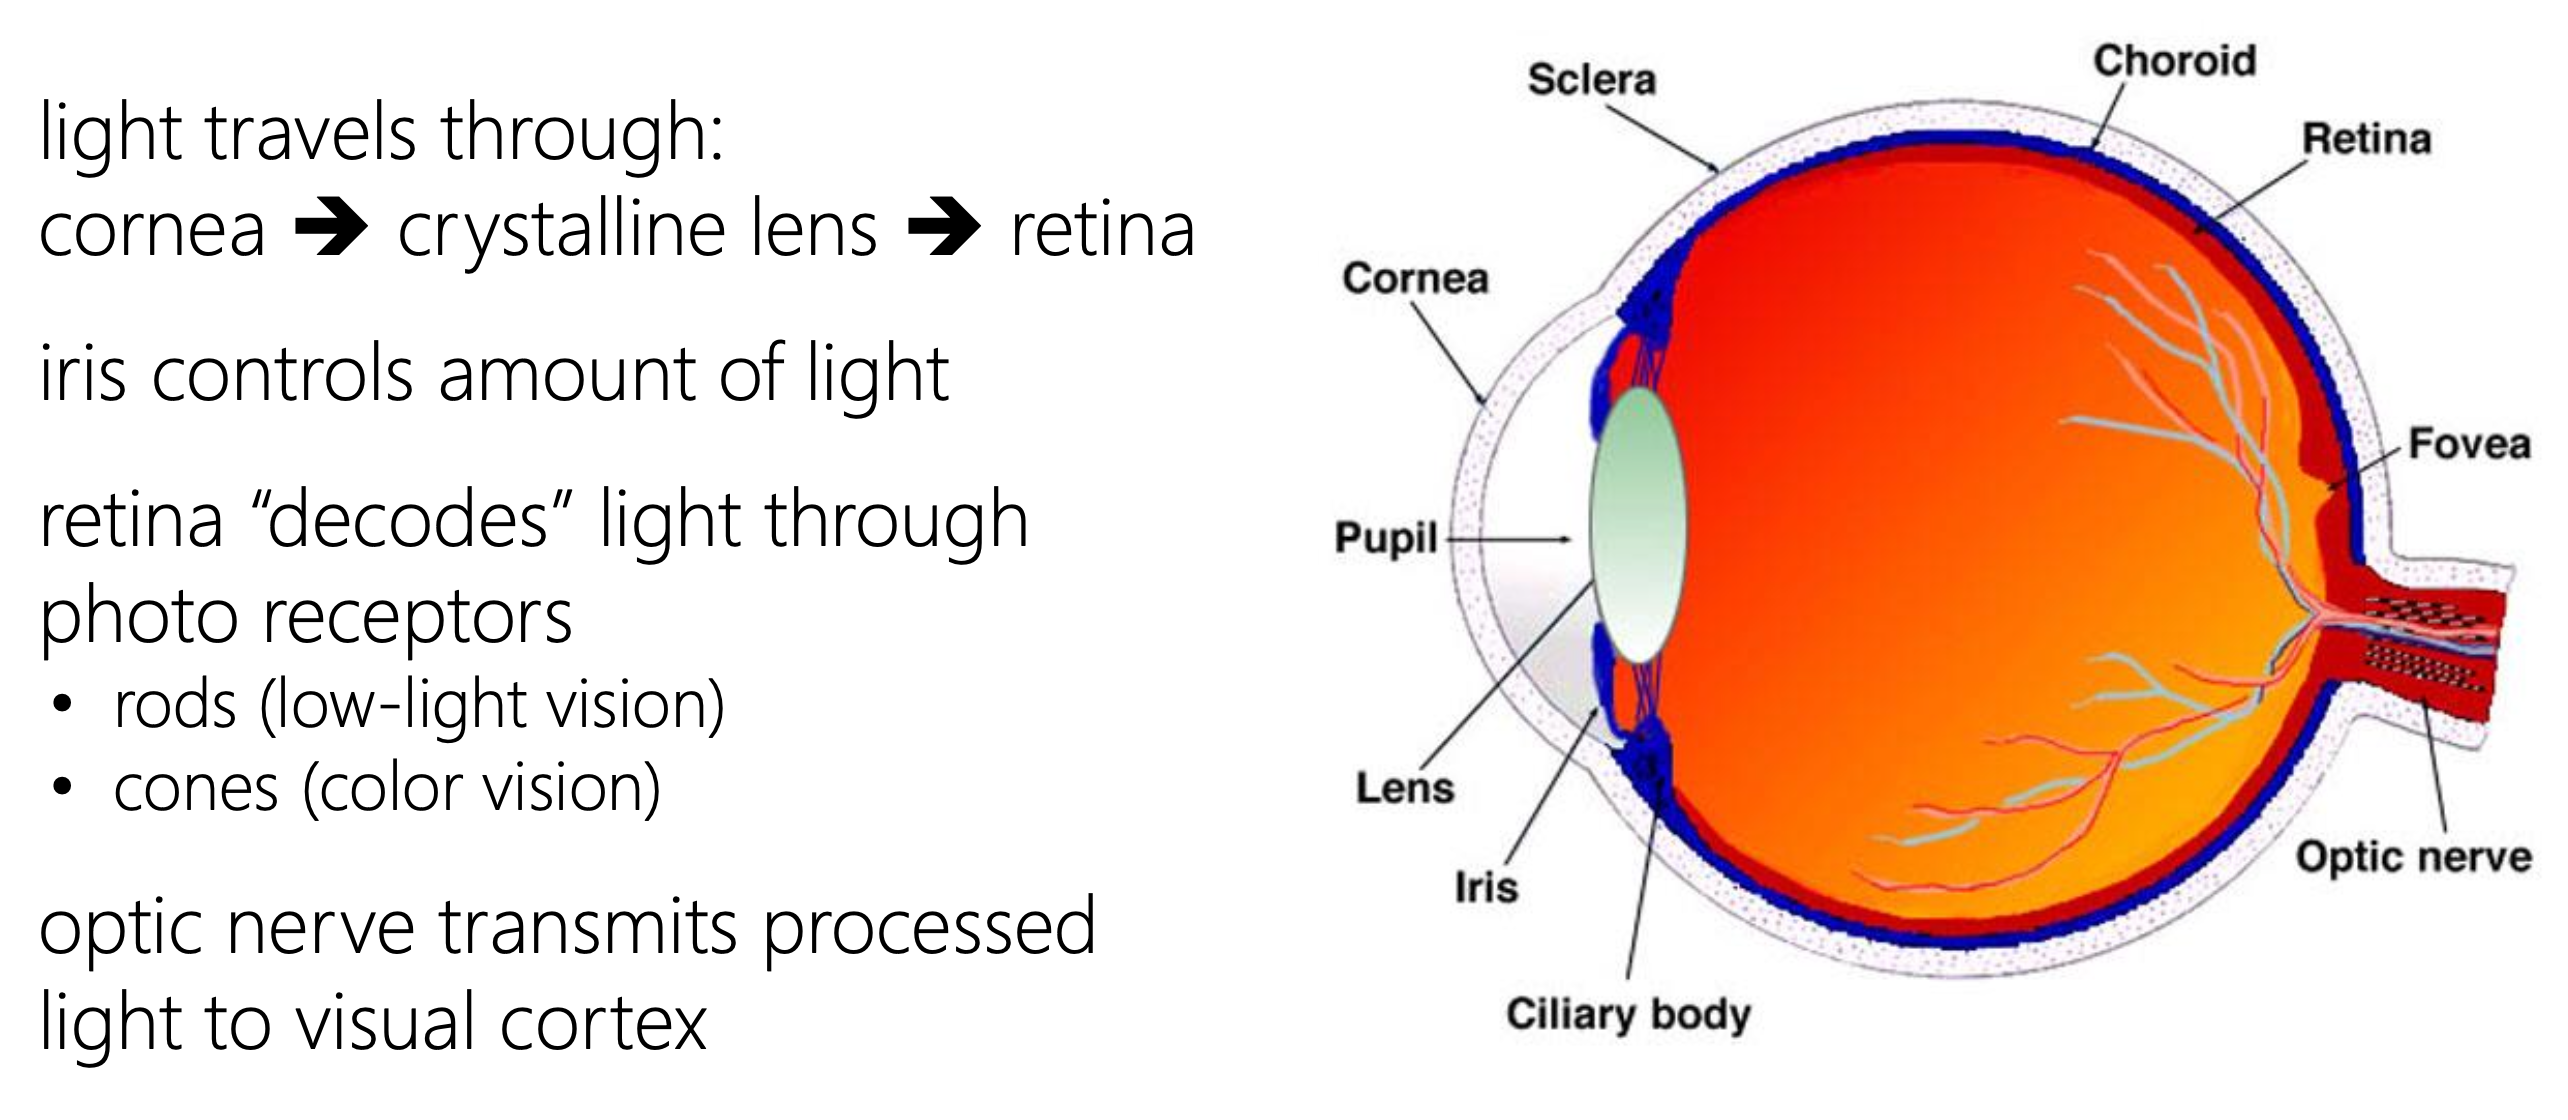
\includegraphics[width=\linewidth]{eye.png}
\end{center}

\medskip

Rods are very light sensitive and have a slow response time. They are located in the periphery of the fovea. 120 million per eye, have maximum sensitivity at 500nm. \medskip

Cones are fast in responding and concentrated at the fovea. 6 million per eye. Three types for blue (S type, 420nm), green (M type, 534nm) and red (L type, 564nm). \medskip


\textit{Visual Field} \smallskip

Sharp vision within 2 degree radius of fovea. Fine detail. Peripheral vision decreases in visual acuity with distance from fovea. Horizontal visual field is 60 degrees nasally and 90 degrees temporally. Verticual visual field is 60 degrees up and 70 degrees down. \medskip

Useful field of view is rather small (1-4 degrees for high character density and max 15 degrees for low character density.) We use this in Foveated Rendering to reduce details in the outer parts (for instance with eye tracking). \medskip

\textit{Eye movement} \smallskip

Saccades are the process of repositioning the fovea. They take around 30ms with an amplitude of max 600degrees per second. Perception is greatly decreased.\medskip

Fixations are dwelling on one point. Fixations happen in between saccades. It takes around 90 percent of the visual time. Take around 150 to 600 ms. \medskip

Gaze movements are context dependent of foreknowledge, attitute, task and predisposition. \medskip

\textit{Reading} \smallskip

Reading is a sequential loop of fixation and saccades. In average around 230ms fixation and 30ms saccades. On average around 300 WPM reading speed. \medskip

\textbf{(Visual) Attention} \smallskip

We have great gaps in our perception. Interpretation is much sparser than one might assume. Perception of objects requires lots of attention. Attention has to be directed. 
Perceptual processor receives and buffers signals. One buffer per sensory channel. Perception time is around 100ms (ranging 50-200ms). \medskip

\textit{Bloch's law} \smallskip

$$R = I * t$$

Where R is response, I is intensity and t is exposure time. For $t < 100$ms, we assume R constant. As a consequence we have limits on frame-rates (min 10Hz). \medskip

\textbf{Cognitive Processor} \smallskip

Connects perceptual system to motor system. Learning, retrieval of facts, decision making, problem solving etc\dots \medskip

Processing time is around 70ms (25-170). Operates on chunks of information. For instance age, parts of a phone number. \medskip

\textit{Short term memory} \smallskip

Working memory, responsible for intermediate products of thinking and representations of perceptual system. Holds activated item from long term memory. Capacity is limited to 5-9 units (augmented by LTM). Pure capacity is around 2-4 units. Decay rate and capacity can be varied depending on strategy etc. but decreases strongly with increased items. \medskip

\textit{Long term memory} \smallskip

Declarative (facts etc.) and procedural (how to do stuff) parts. Practically unlimited capacity with no decay time. Retrieval depends on associations with for instance external stimuli. It is fast-read, slow-write. 

\textit{Designing for memory} \smallskip

We try to design for memory through grouping of related functionalities and usage of familiar structures. We also use recognition instead of recall. \medskip

\textbf{Motor Processor} \smallskip

The average processing time is the sum of time needed for the perceptual, cognitive and motor processor. We differentiate between an open (no perceptual control, motor processor takes around 70ms) and a closed loop (perceptual system controls movement, ca 250ms). \medskip

\textit{Fitt's Law} \smallskip

Models throughput in aimed movements such as reaching for a control in the cockpit or clicking on icons with a mouse. Is very powerful and widely used. Holds in many circumstances, also under water and intoxicated. Allows for comparison among different experiments. \medskip

Originally the task was to touch a centerplate with a pencil, without touching the error plates on the sides. Generally the task is to predict the time to hit a target as a function of distance and size. \medskip

Index of difficulty
$$I_D = log_2(2D/W)$$

\textit{Index of Performance or Throughput} \smallskip

ID = information (nr of bits) required to specify movement (amplitude within given tolerance)\smallskip
IP = index of performance. 

$$IP = ID / MT $$(is in bits/sec)
Depends on input device and limb. \smallskip
Movement time MT

$$MT = a + b * ID$$
$$MT = a + b *log_2(2D/W)$$

In the end we can use the different MTs to estimate a regression on ID and MT (estimate a and b of line). \medskip

\textit{Fitt's Law implications} \smallskip

We find that doubling the distance adds roughly a constant to execution time (Logarithmic nature of the law). Doubling the target width is roughly equal to halving the distance (implicated by D/W term in the formulation). \medskip

\begin{center}
	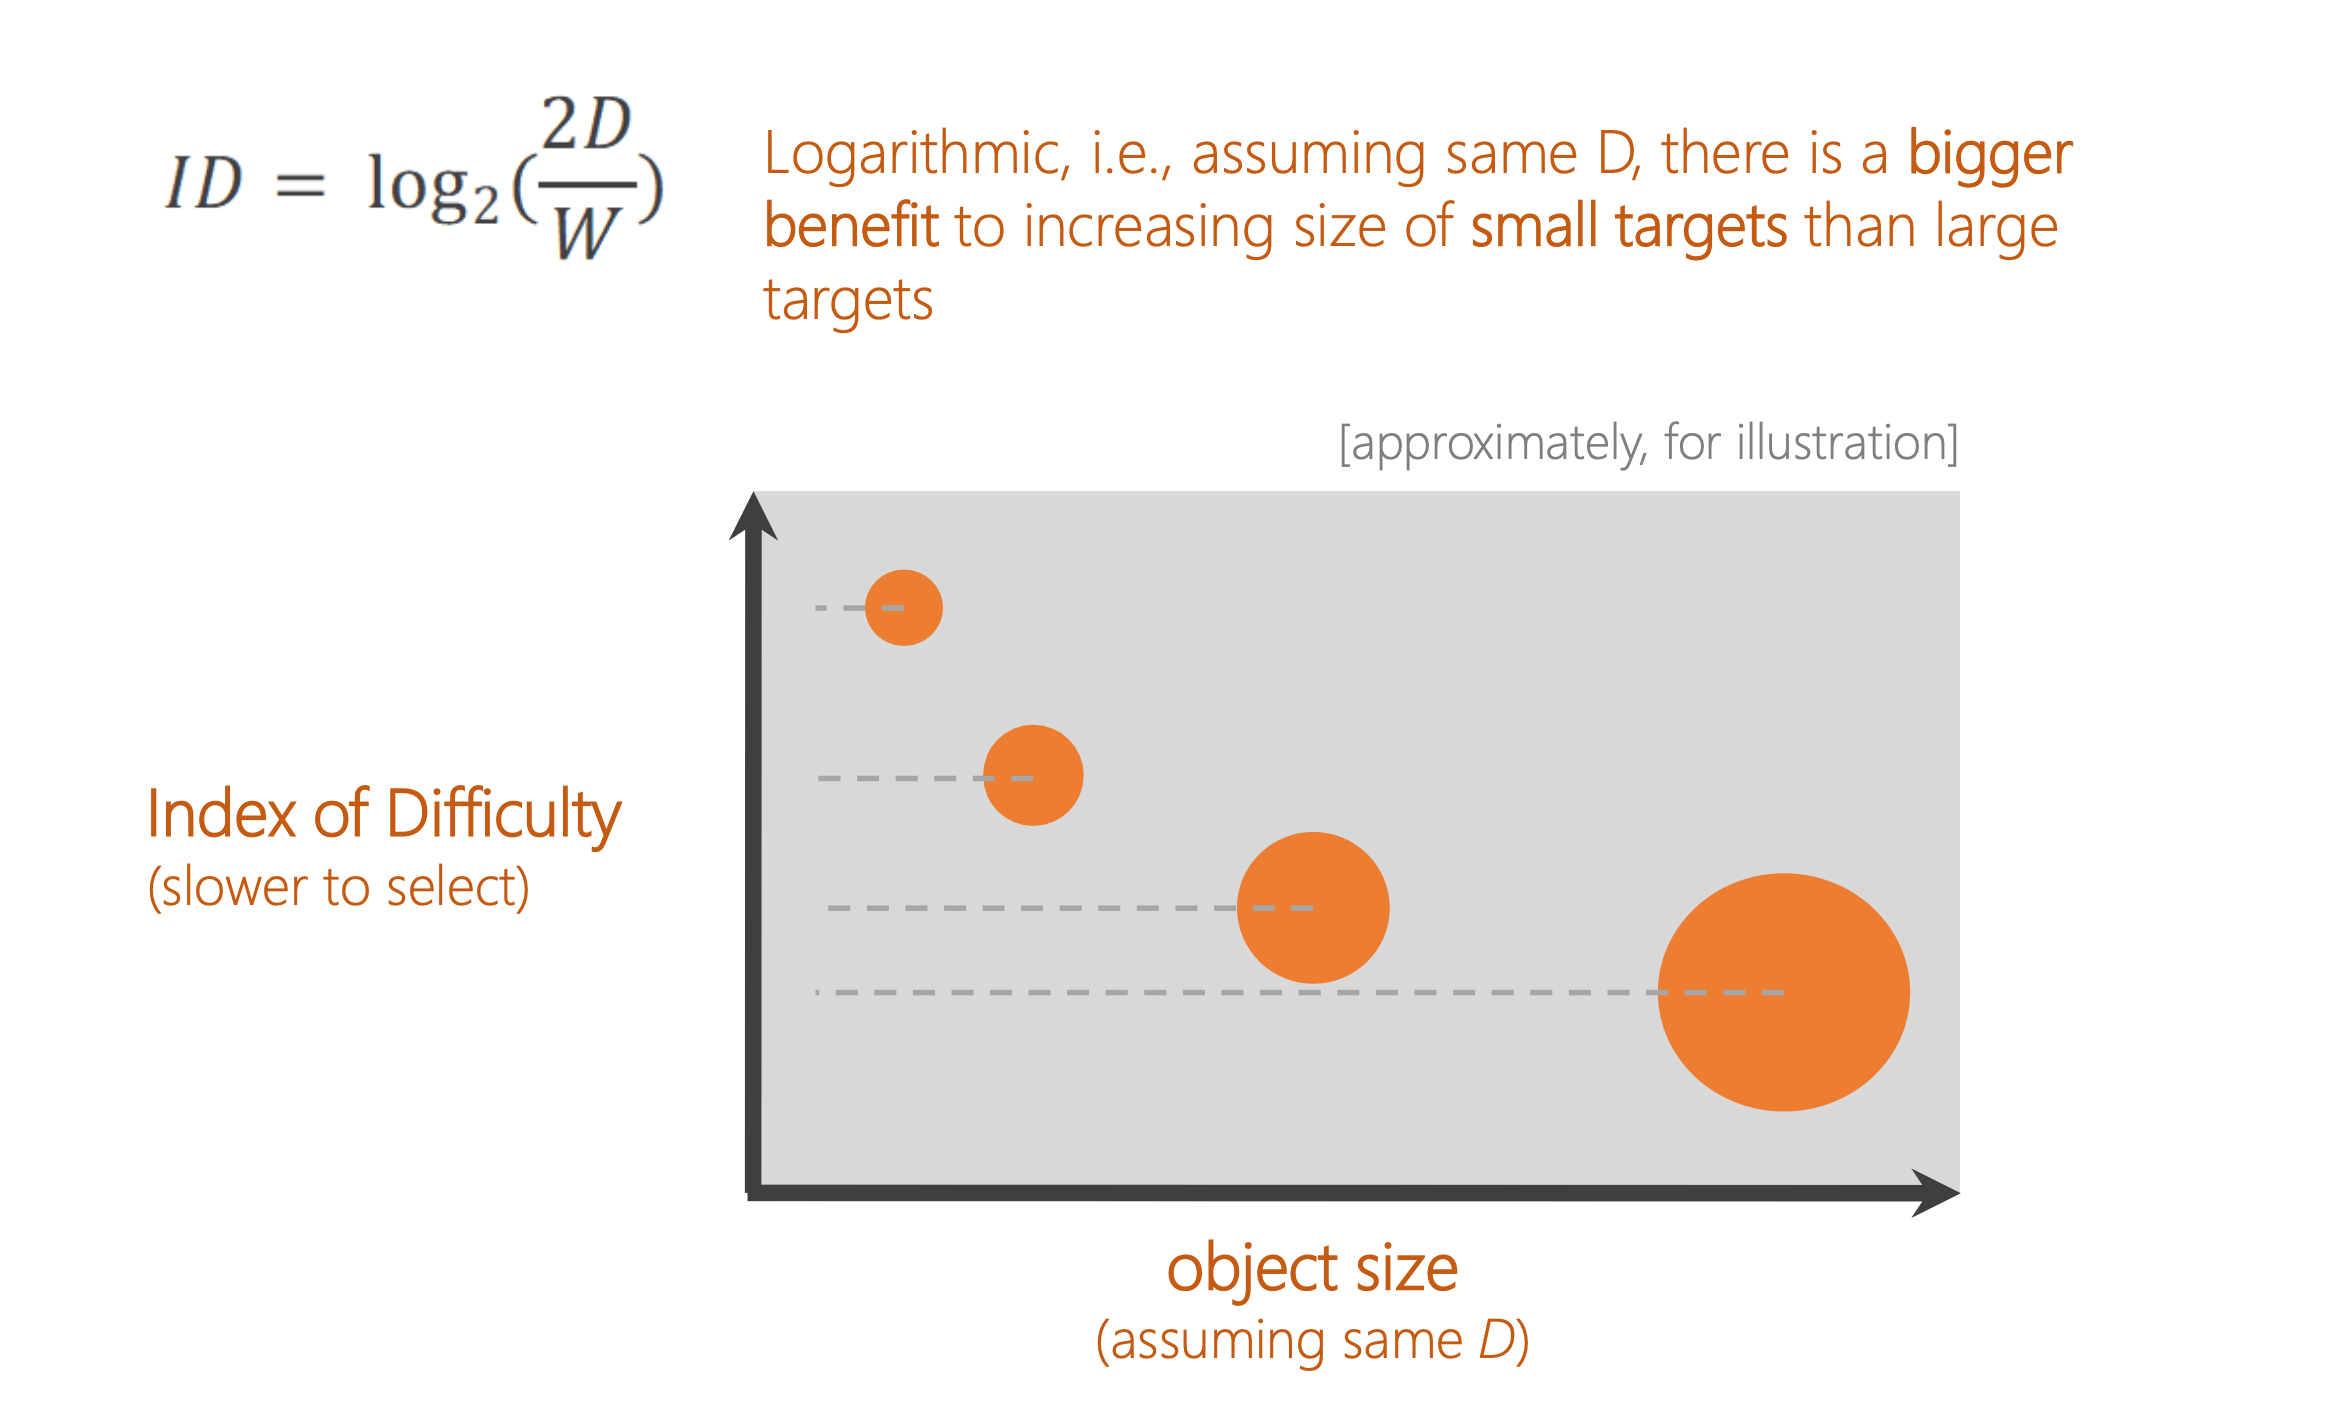
\includegraphics[width=\linewidth]{fitss_law.png}
\end{center}

\textit{Fitt's Law in practice} \smallskip

We can add the last pixel of buttons on the left side, to increase the effective Width of "almost infinite". \smallskip

Larger fields can be clicked more easily. \medskip

\textit{Application: Compare input devices} \smallskip

Compare mouse, trackball and stylus in speed. Use pointing and dragging as actions. This corresponds to finding $a$ and $b$ in the formula for $MT$. The we can compare the index of performance (throughput). We can then use this information to design an "optimal" UI. \medskip

\textit{Limitations of Fitts' Law} \smallskip

Fits law does not: 


\begin{itemize}[itemsep=-5pt, topsep=0pt, leftmargin=*]
    \item consider body asymmetries (right vs. left hand flexion vs. extension)
    \item address parallelization strategies (use multiple finger, hands)
    \item include any cognitive factors (reaction time, visual search time etc.)
\end{itemize}
\medskip

\textbf{Bandwidth} \smallskip


\begin{center}
	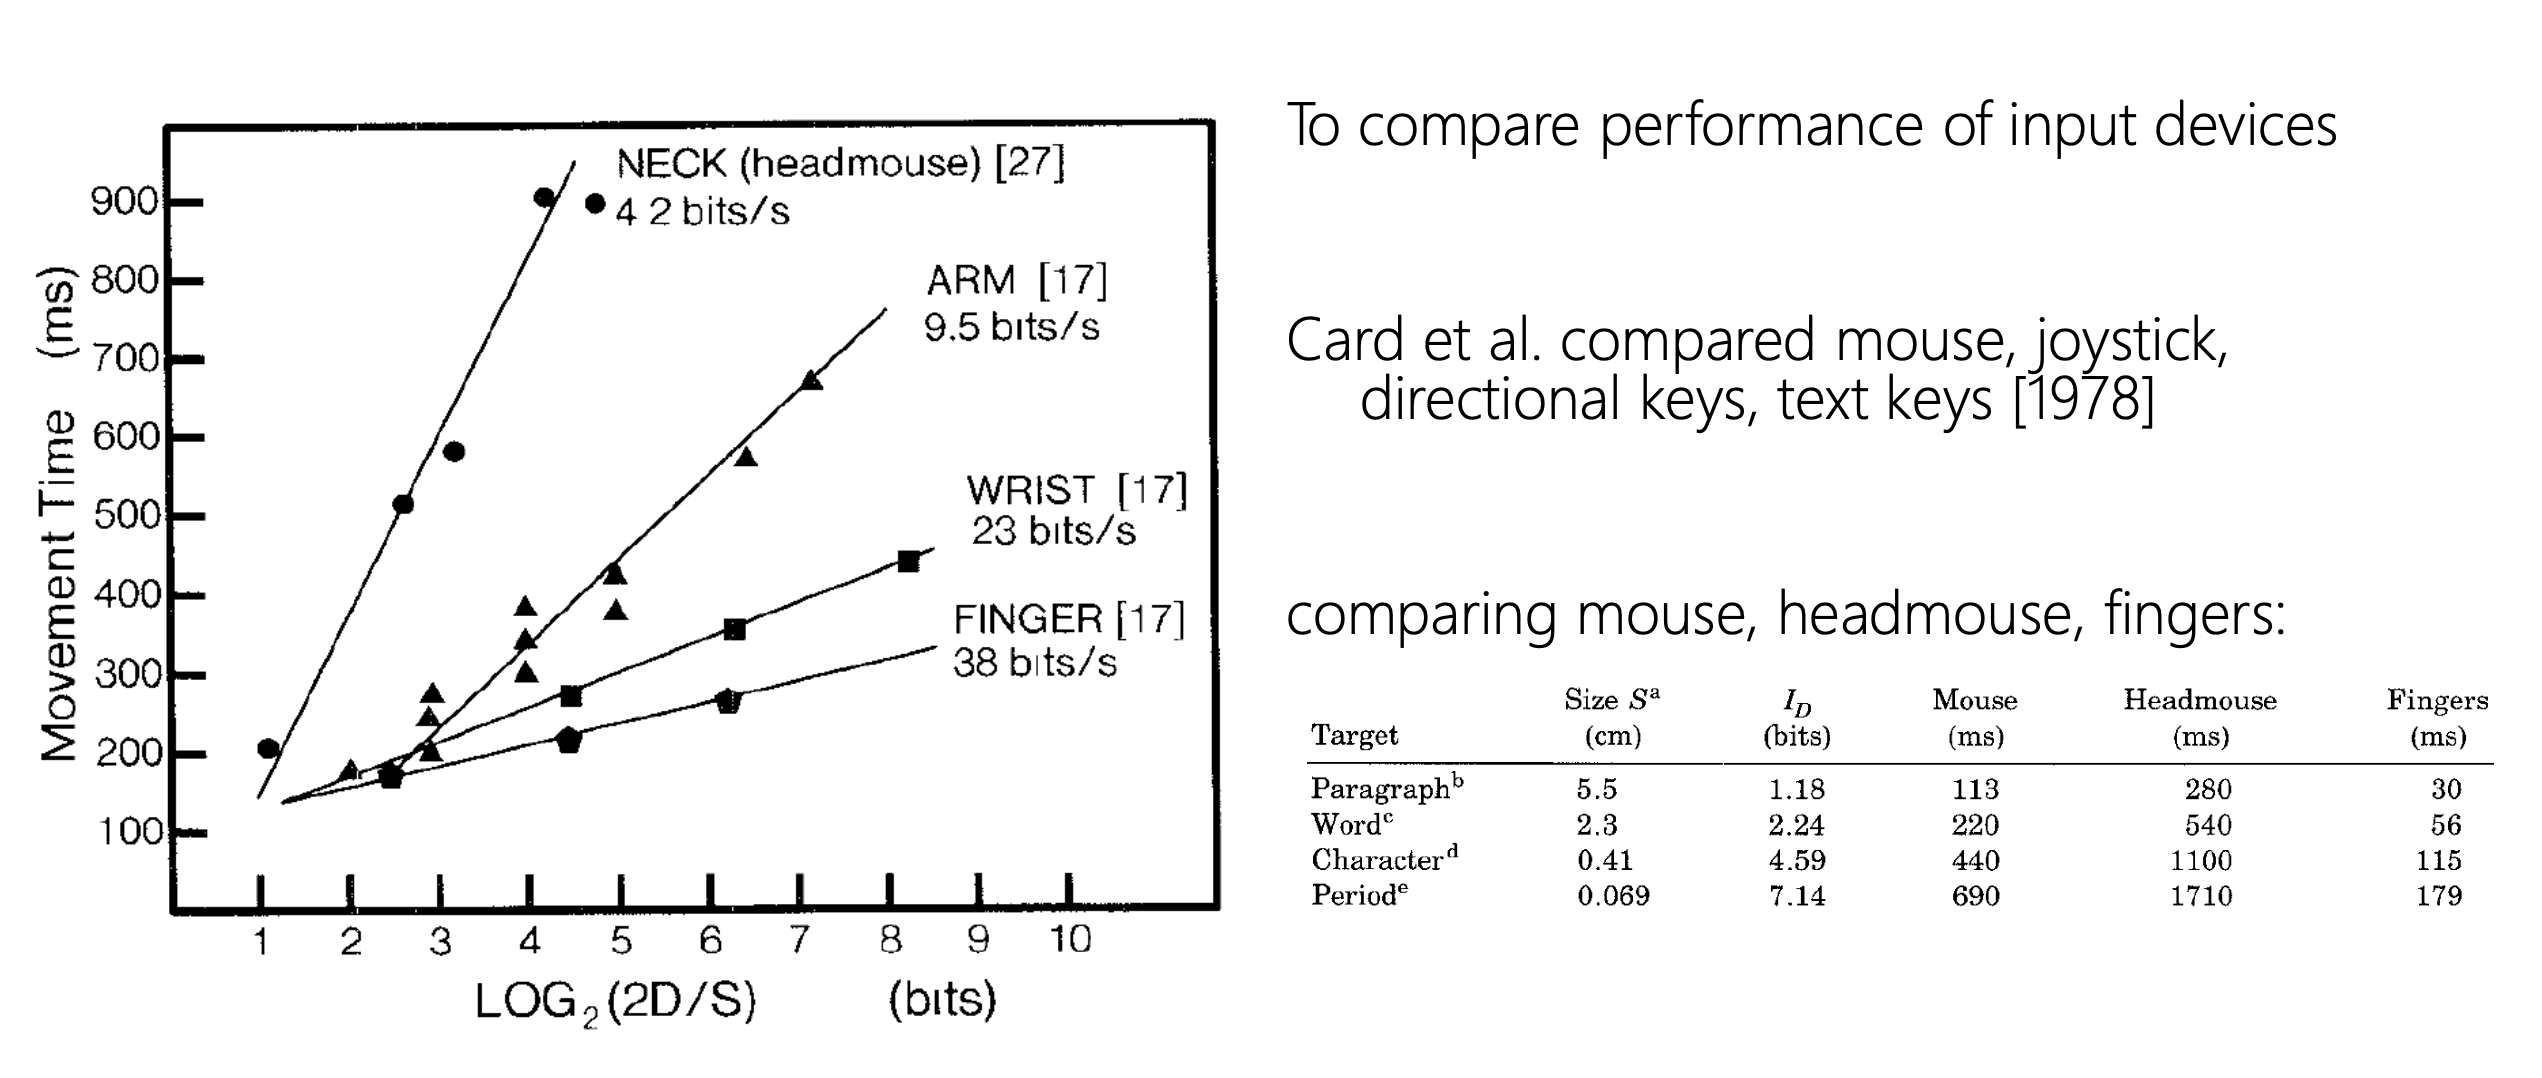
\includegraphics[width=\linewidth]{bandwidth.png}
\end{center}

\medskip

Performance of use depends on human (bandwidth of muscle groups), application (precision requirments of the task) and device (effective bandwidth of input device). \medskip


\textbf{From Model Human Processor to Fitt's Law} \smallskip

\textit{Visual and Proprioceptive Feedback Loop} \smallskip

First we observe handposition, then we plan the movement, we perform the hand movement and finally asses the error to expected position. This is a loop and gets repeated until desired movement is finished. 


\begin{center}
	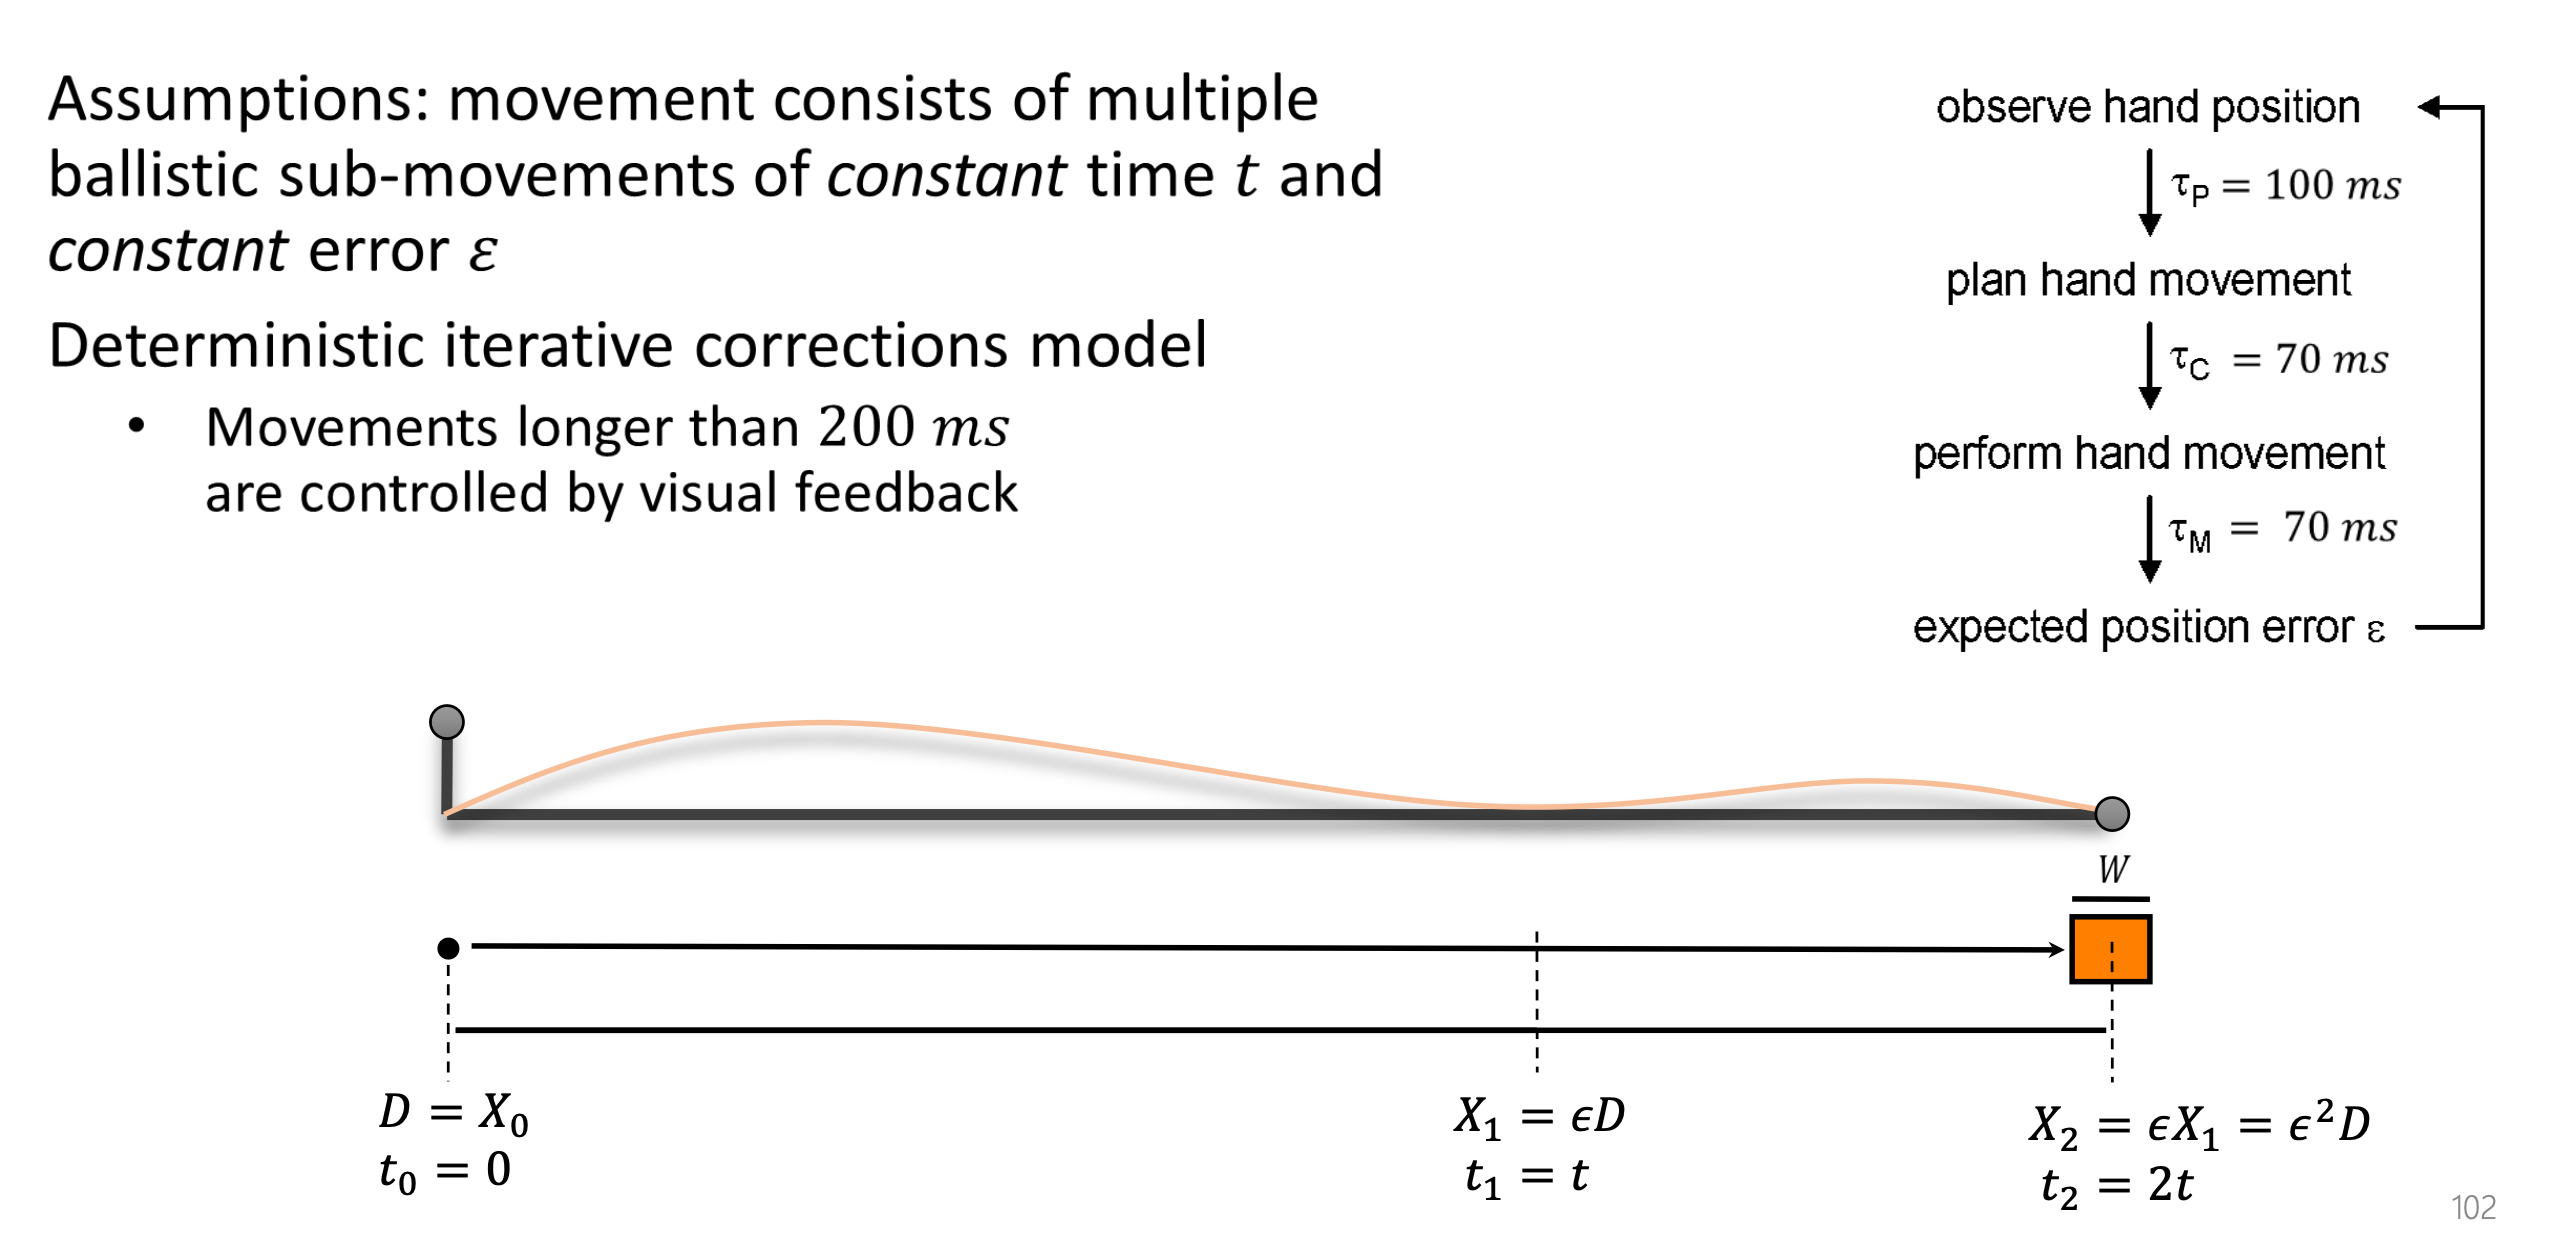
\includegraphics[width=\linewidth]{visual_feedback_loop.png}
\end{center}

We know from MHP that one cycle through all processors is around 300ms. If n is the times we go through loop, the final time then is
$$n \times (\tau_p + \tau_c + \tau_M)$$

After the first cycle we have:
$$X_1 = \epsilon X_0 = \epsilon D$$
In the second cycle:
$$X_2 = \epsilon X_1 = \epsilon(\epsilon X_0)= \epsilon^2 D$$

$n^{th}$ cycle :
$$X_n = \epsilon^n D $$

We stop the movement when:

$$\epsilon^n D \leq \frac{1}{2} W$$

We solve for n:
$$ n = -log_2(\frac{2D}{W})/log_2\epsilon$$

We insert into formula for movement time: 

$$MT = n \times (\tau_p + \tau_c + \tau_M)$$

$\Rightarrow$

$$ MT = \frac{\tau_p + \tau_c + \tau_m}{-\log_{2} \varepsilon} \cdot \log_{2} \left( \frac{2D}{W} \right) $$

$$ MT = I_M I_D $$

$$ I_M = \text{Index of motion} \left( \frac{\text{sec}}{\text{bits}} \right) $$


\columnbreak

























\section{Visual Perception}

\textbf{Gestalt principles}


Gestalt psychology was founded in the 1920s by Max Wertheimer and others. It is about the perception of groups, patterns and objects. \medskip

\textit{Four key principles}
\begin{multicols}{2}
    \begin{itemize}[itemsep=-5pt, topsep=0pt, leftmargin=*]
        \item Emergence
        \item Multistability
        \item Reification
        \item Invariance
    \end{itemize}
\end{multicols}

\textit{Laws of grouping}
\begin{itemize}[itemsep=-5pt, topsep=0pt, leftmargin=*]
    \item Proximity (close objects belong to group)
    \item Similarity (similar appeareance belong to group)
    \item Closure (humans prefer to see complete figures)
    \item Symmetry (Symmetric objects form groups around the center)
    \item Figure and ground (users tend to seperate images to fore- and background)
    \item Continuity (Objects that intersect are perceived as continous rather than individual objects)
    \item Past experience (Based on past experience group objects together)
\end{itemize}
\medskip

\textbf{Feature integration theory} \smallskip

Availability of visual information is limited. Full visual acuity is only available in foveal area. Peripheral vision provides limited information. 
This is why FIT suggests stimuli that are registered early and automatically. 

\begin{center}
	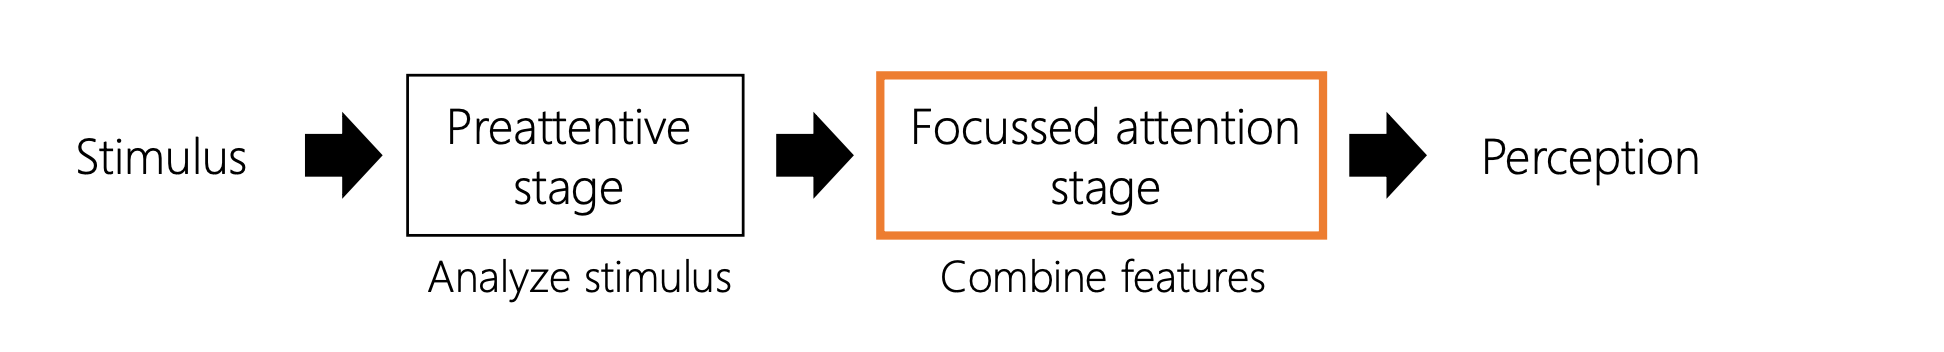
\includegraphics[width=\linewidth]{feature_integration_principle.png}
\end{center}
\begin{center}
	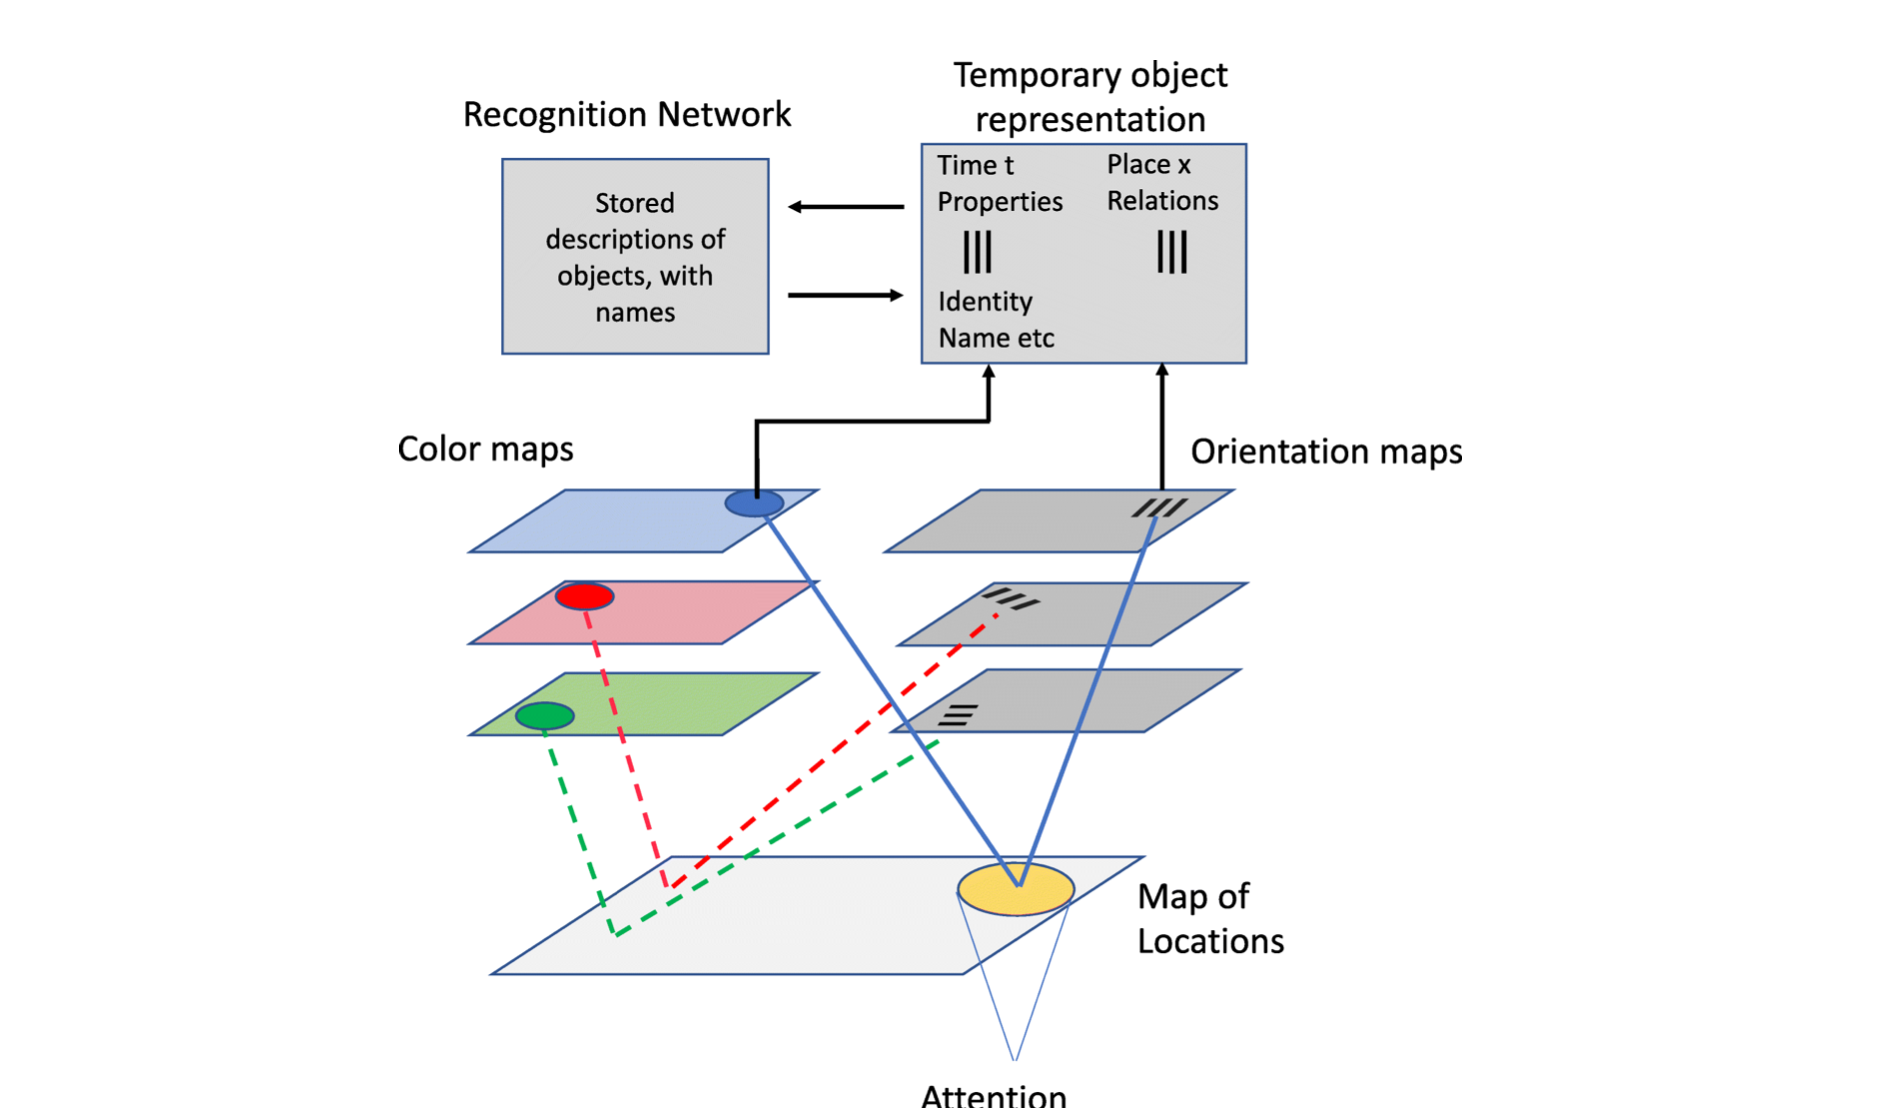
\includegraphics[width=\linewidth]{fit_2.png}
\end{center}

Theory is based on the process of selective attention. Is useful but certainly limited in certain aspects. FIT primarily concerns bottom-up activation. Top-down activation through memory and expectation. \medskip

\textbf{Selective Attention} \smallskip

There is an ongoing debate about Early / Late selection. The early selection model has been proposed earlier and mainly relies on the idea of an early "bottleneck" in the attentional process given by perception. 
It also assumes that focussed attention can prevent distractor processing at an early stage\medskip

Late selection was proposed later and assumes unlimited perception and the automatic discrimination of relevant and irrelecant stimuli. 
It assumes that later processes such as memory or behavior are the processes with selected attention. \medskip

\textbf{Perceptual Load Theory} \smallskip

Sees perception as a process with limited capacity. This is in line with the early selection views. PLT also assumes that all stimuli are automatically processed until capacity is filled. \smallskip

\textit{Example experiment on PLT}
\begin{center}
	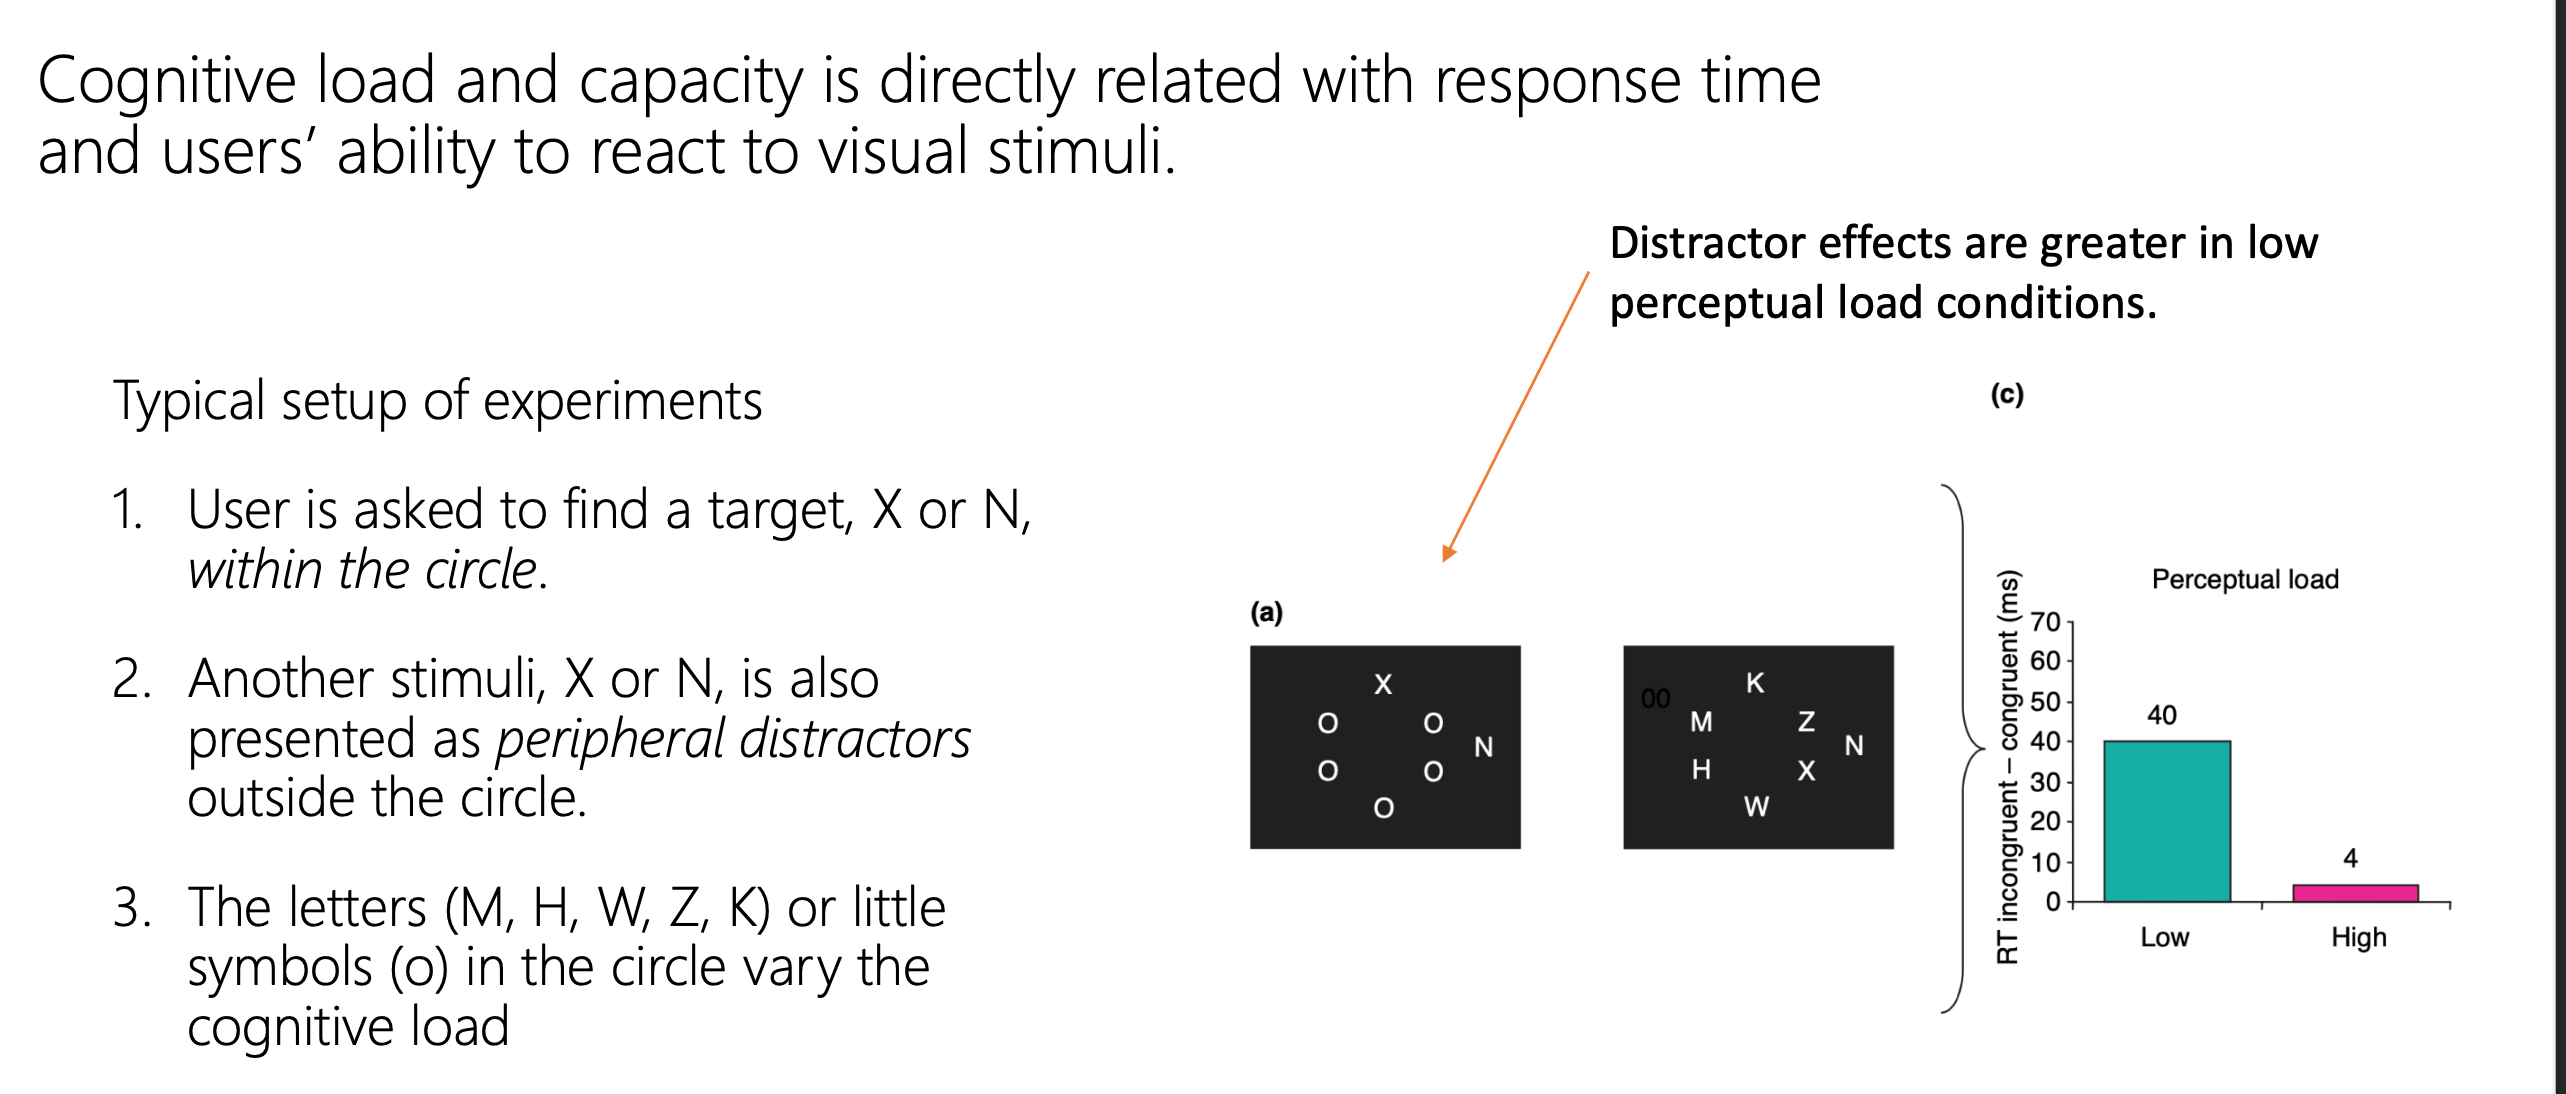
\includegraphics[width=\linewidth]{plt_experiment.png}
\end{center}

\textit{Takeaways on PLT}

Users ability to react to stimuli is related to its context. High load leads to more focus and less distraction. Low load leads to quicker distraction.\medskip

\begin{center}
	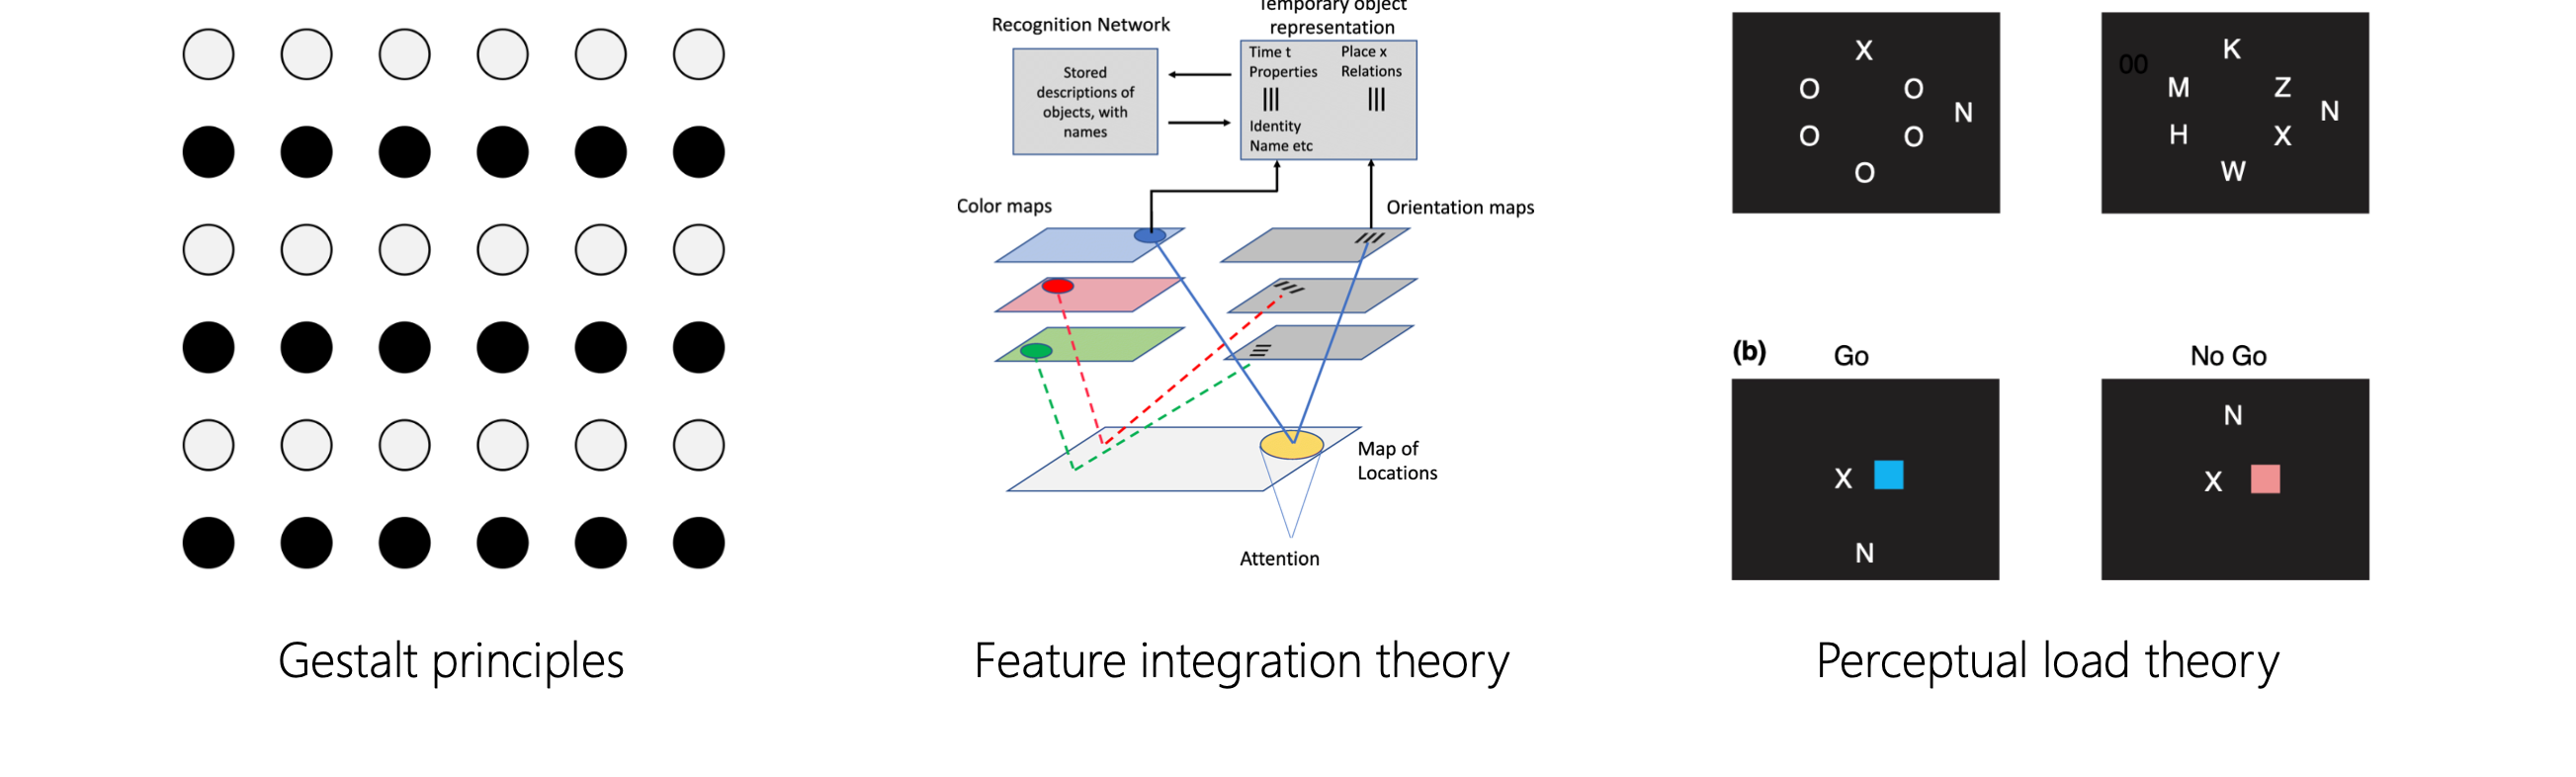
\includegraphics[width=\linewidth]{models_of_perception.png}
\end{center}

\textbf{Visual Saliency} \smallskip

The context of objects popping-out as pre-attentive for selection. Assumes that feature maps are computed in parallel and combined. The computed maps yield a saliency map. Assumes that the "Winner-takes-it-all".
Assumes that this sequential processing is based on inihibition of return. \medskip

Example is given by an experiment where different skins are compared and snake skin resulted in significantly higher brain activity measured over EEG. \smallskip

With visual saliency we can predict users' gate and importance. It is mainly bottom-up and therefore feature based. Top-down saliency is challenging, however task and load influence the saliency. \medskip

If there is too many competing features, clutter will occur. \medskip


\begin{center}
	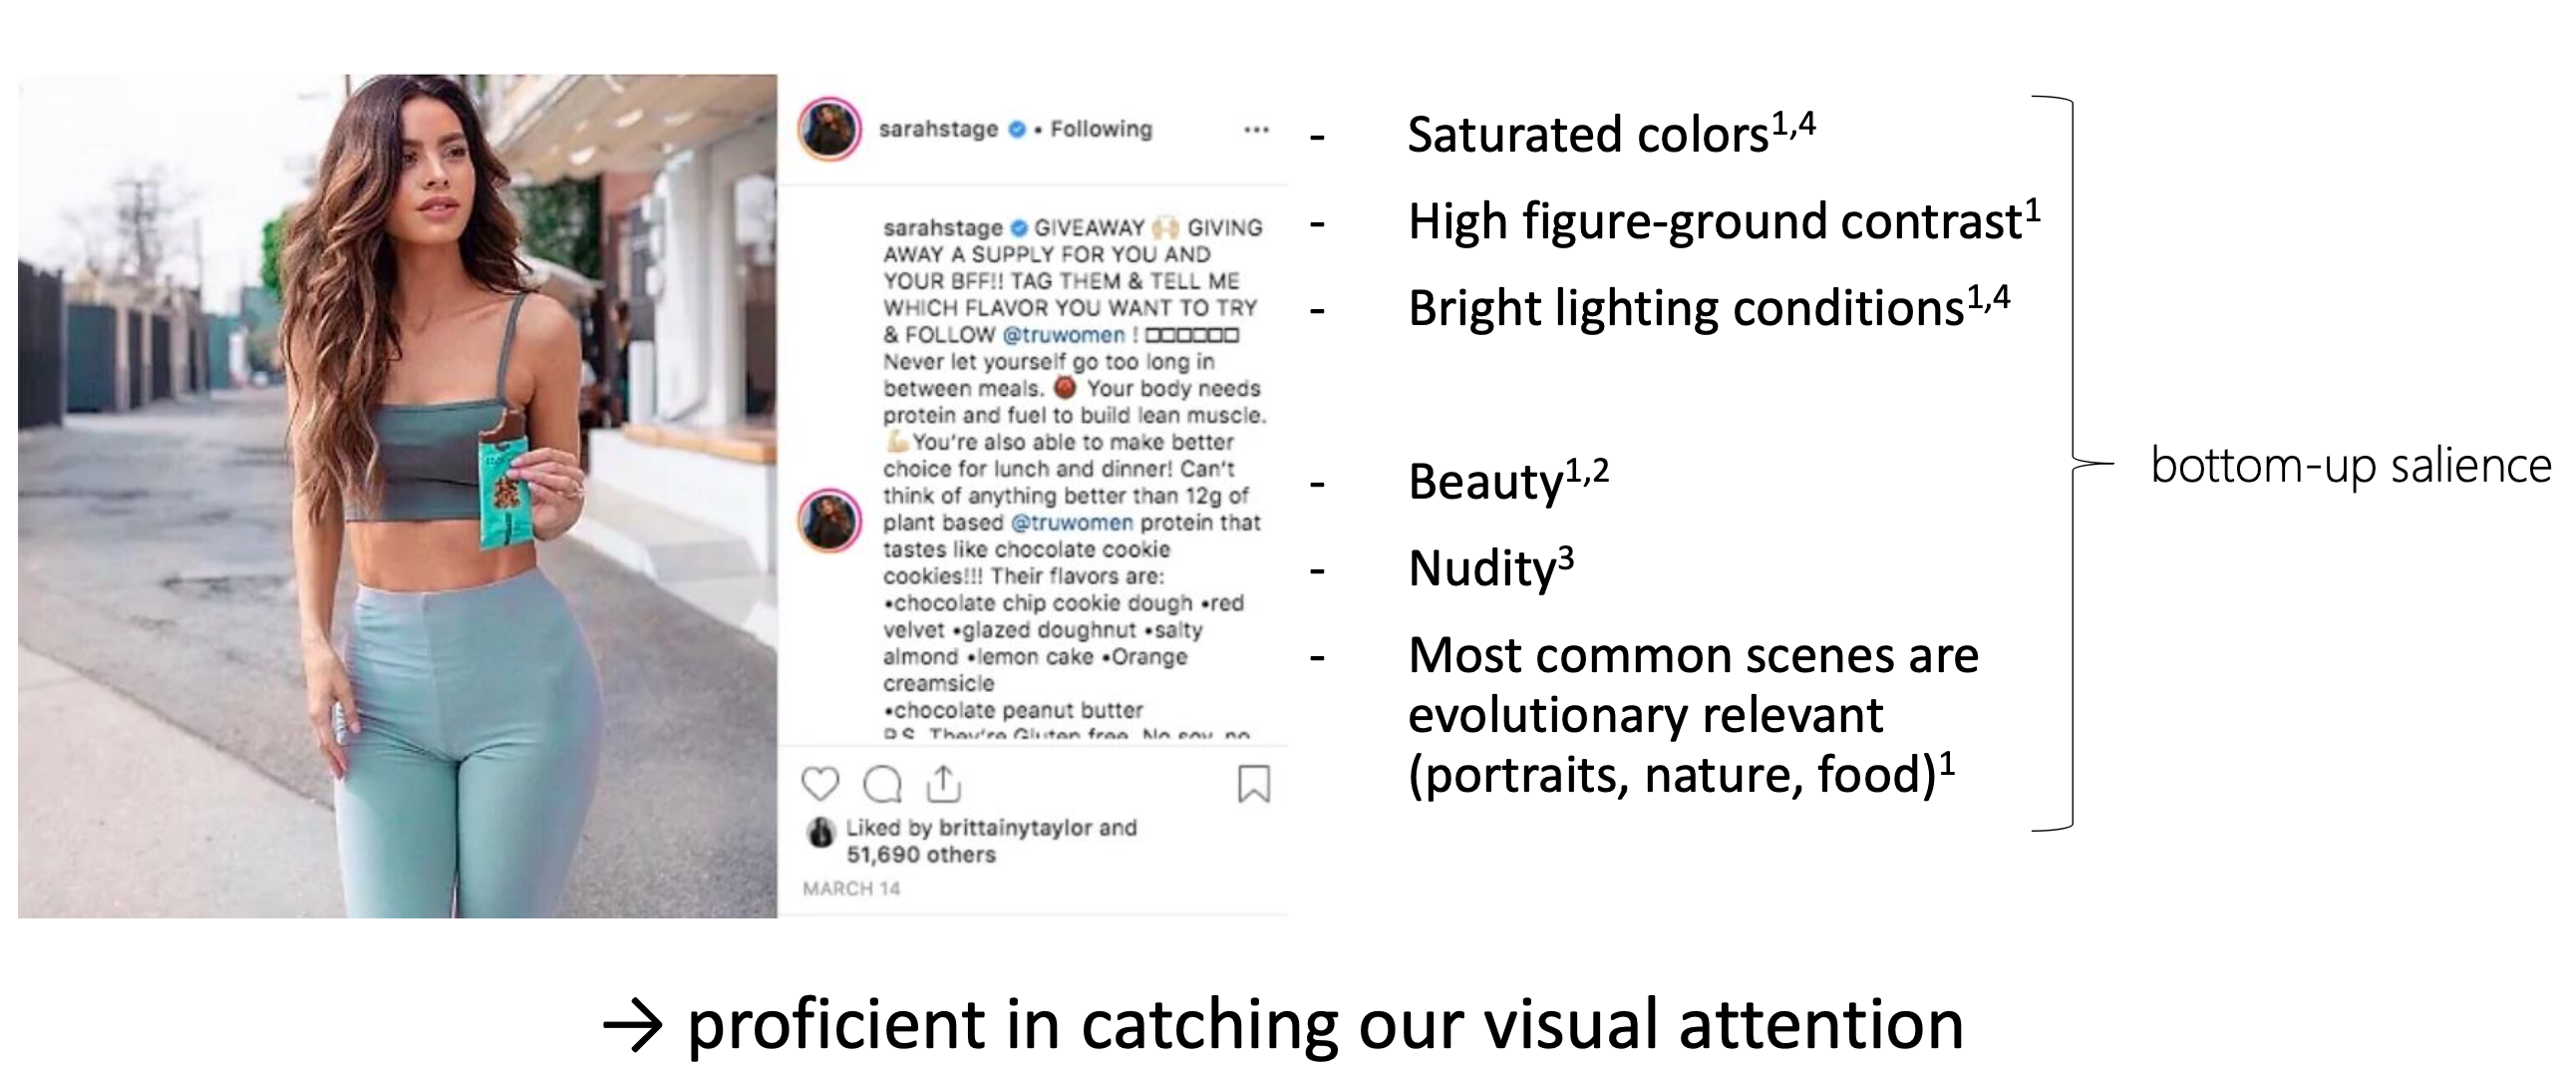
\includegraphics[width=\linewidth]{visual_saliency_example.png}
\end{center}



\textbf{Visual Search} \smallskip

The process that decides where humans look next. 

\begin{enumerate}[itemsep=-5pt, topsep=0pt, leftmargin=*]
    \item Guided Search (rules exist on priorities for items or areas int the scene)
    \item Bounded rationality (selection of actions based on expected utility bunder uncertainty)
\end{enumerate}

\medskip

\textit{Guided Search} \smallskip

\begin{enumerate} [itemsep=-5pt, topsep=0pt, leftmargin=*]
    \item Calculate the distance (eccentricity) to the current fixation location for each item
    \item Given eccentricity, decide which items and features are available to visual representations
    \item Calculate bottom-up saliency for each item
    \item Calculate top-down saliency for each item
    \item Sum up bottom-up and top-down activations and select the ones with highest activation
\end{enumerate}

\textit{Bounded Rationality} \smallskip

Assumes that humans take the action with satisfactory expected utility given their constraints. 

\begin{center}
	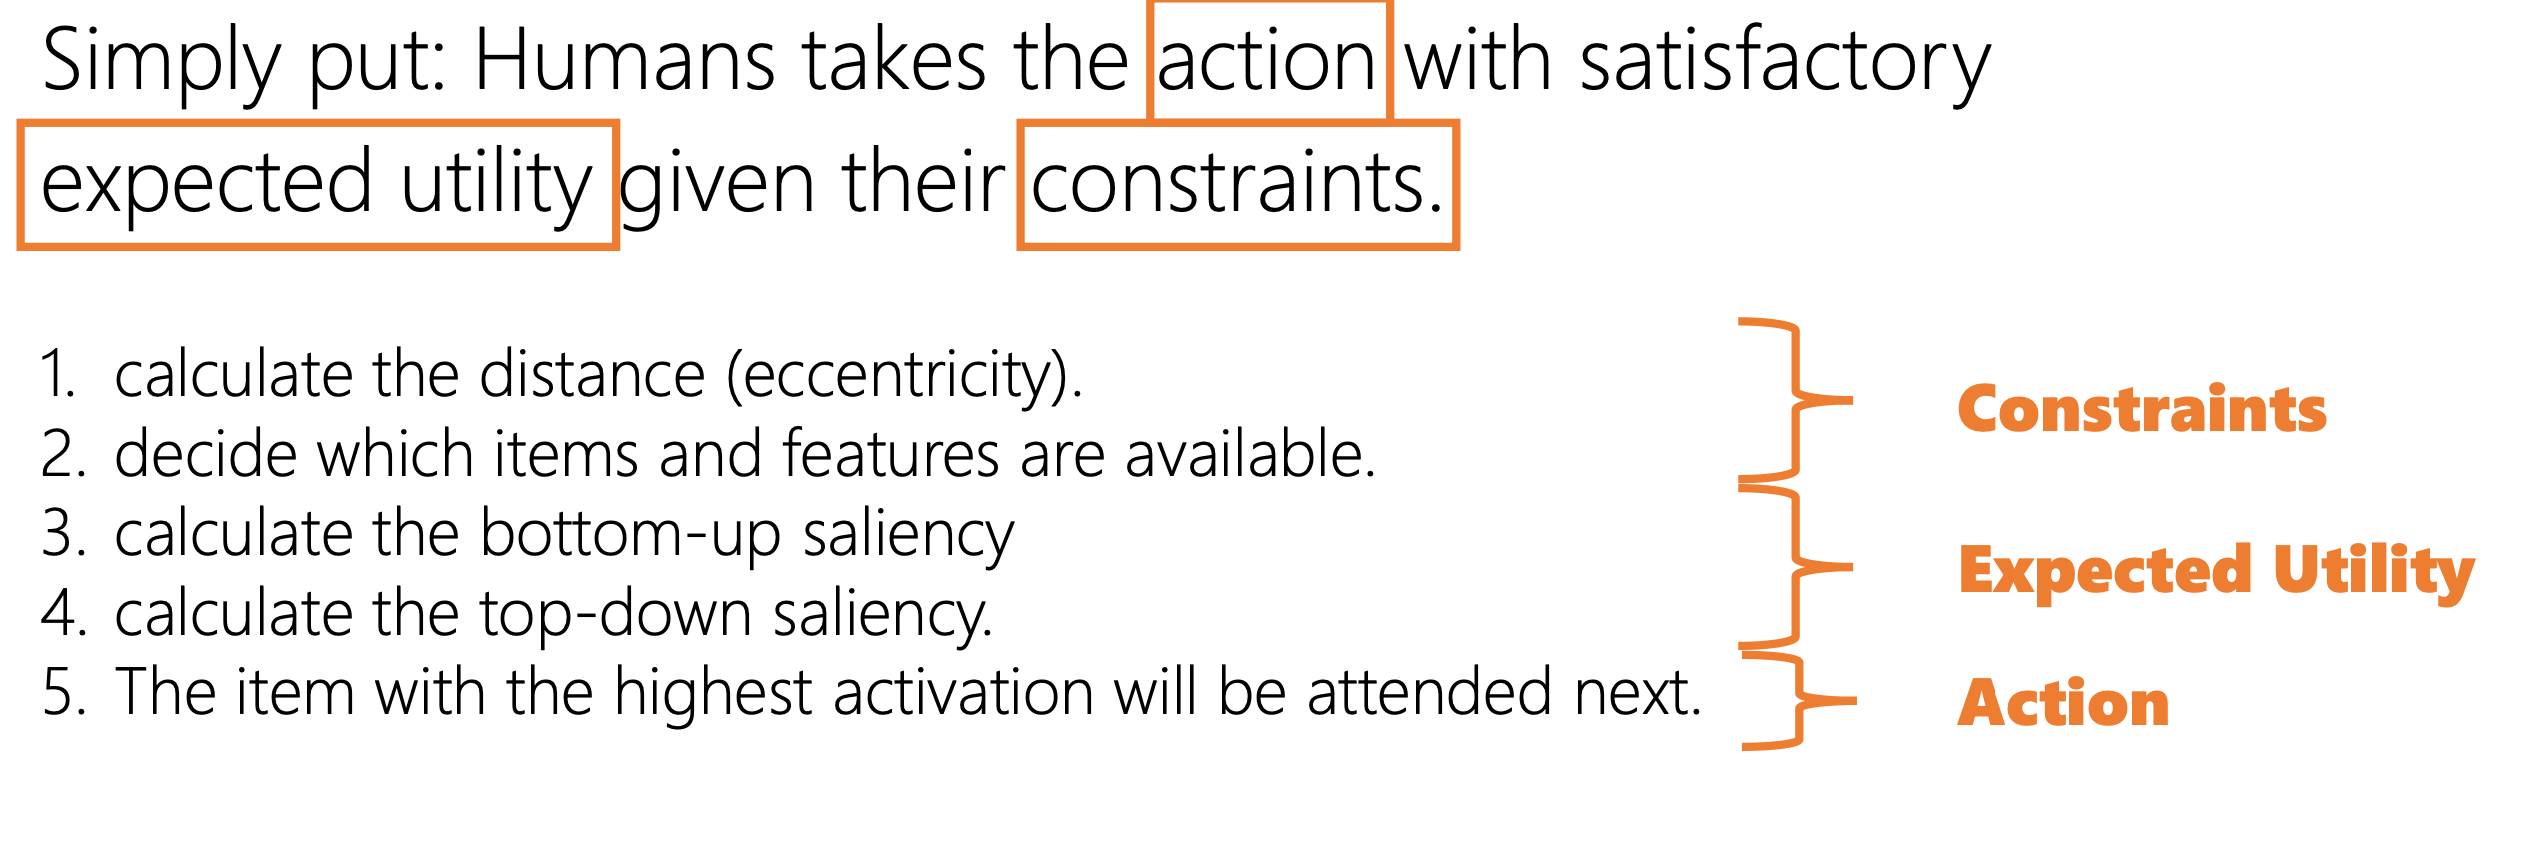
\includegraphics[width=\linewidth]{bounded_rationality.png}
\end{center}

Both visual saliency and search behavior are important for user interfaces and computational design. \medskip

\textbf{Application in HCI} \smallskip

\textit{Aalto interface metrix (AIM)} \smallskip

Combination of empirical models and metrics of user perception and attention. 
Quantifies user experience, complements and removes guesswork. \medskip


\textit{Online UI adaption} \smallskip

Is a tool to measure spatially and semantically relevant labels. Measures pre-attentive object features. It is also possible to distinguish pre-attentive and attentive object features. \medskip

There are also many more tools and applications that make use of these concepts. 

\columnbreak




\section{Input}

\textbf{Input Devices}

Fitt's law for performance evaluation of input devices, but how to distinguish in functionality and specific metric? Answer is systematization. 
In general input devices enable to engange in dialogue with a computer or a machine. This dialogue is not in natural language. 
Dialogue is between fundamentally dissimilar agents-both in perception and processing. \medskip

"It's a transducer from the physical properties of the world into logical values of the application." \medskip

\textbf{Fitts' Law in 2D}

\begin{center}
	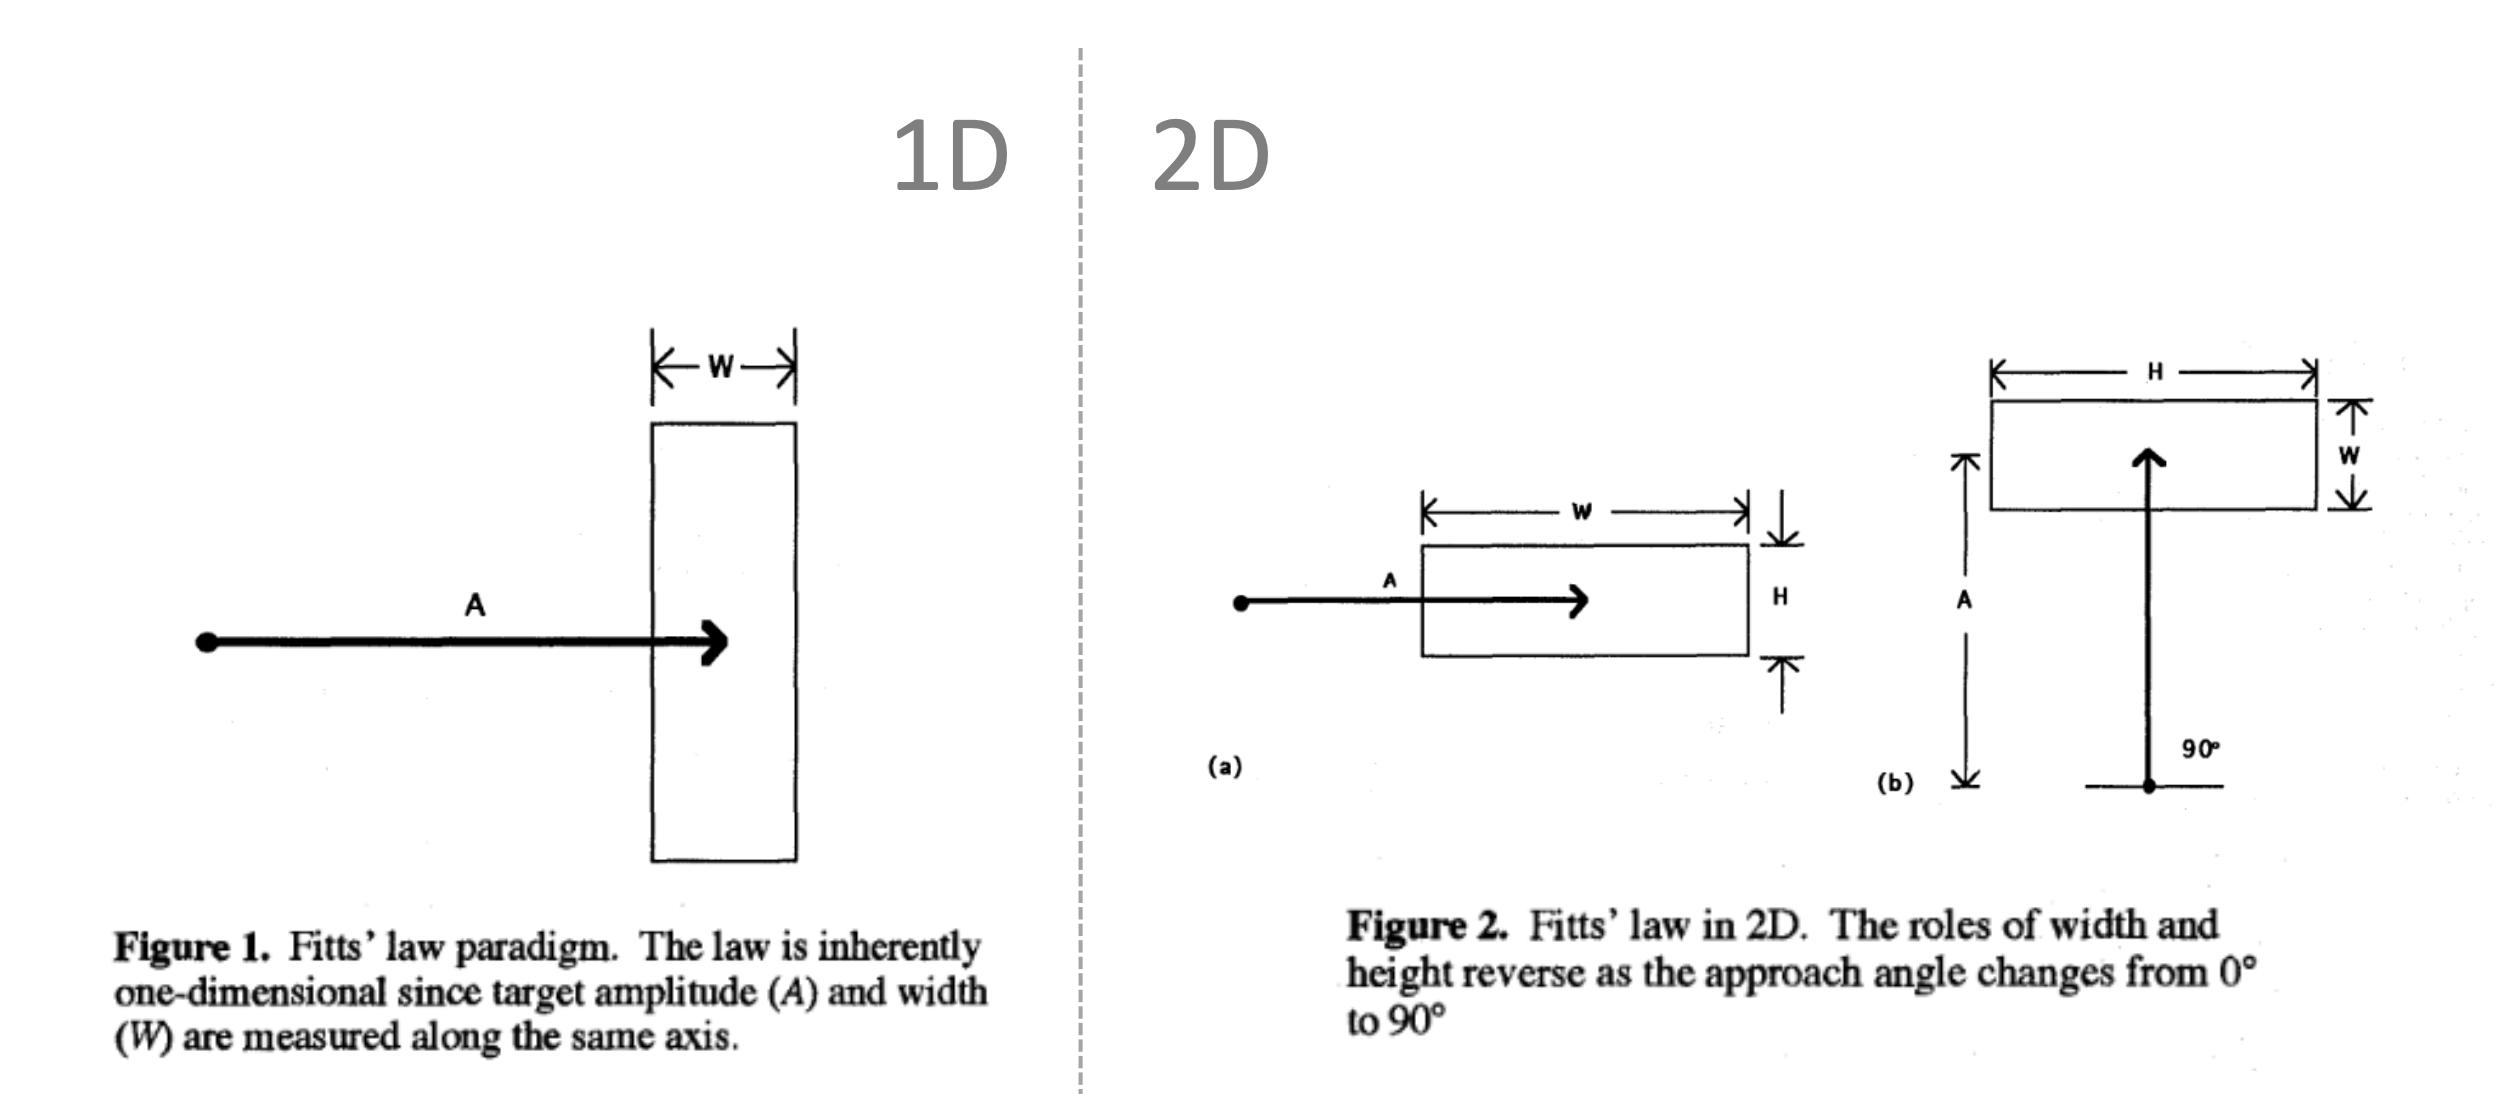
\includegraphics[width=\linewidth]{fitts_law_2d.png}
\end{center}

\begin{center}
	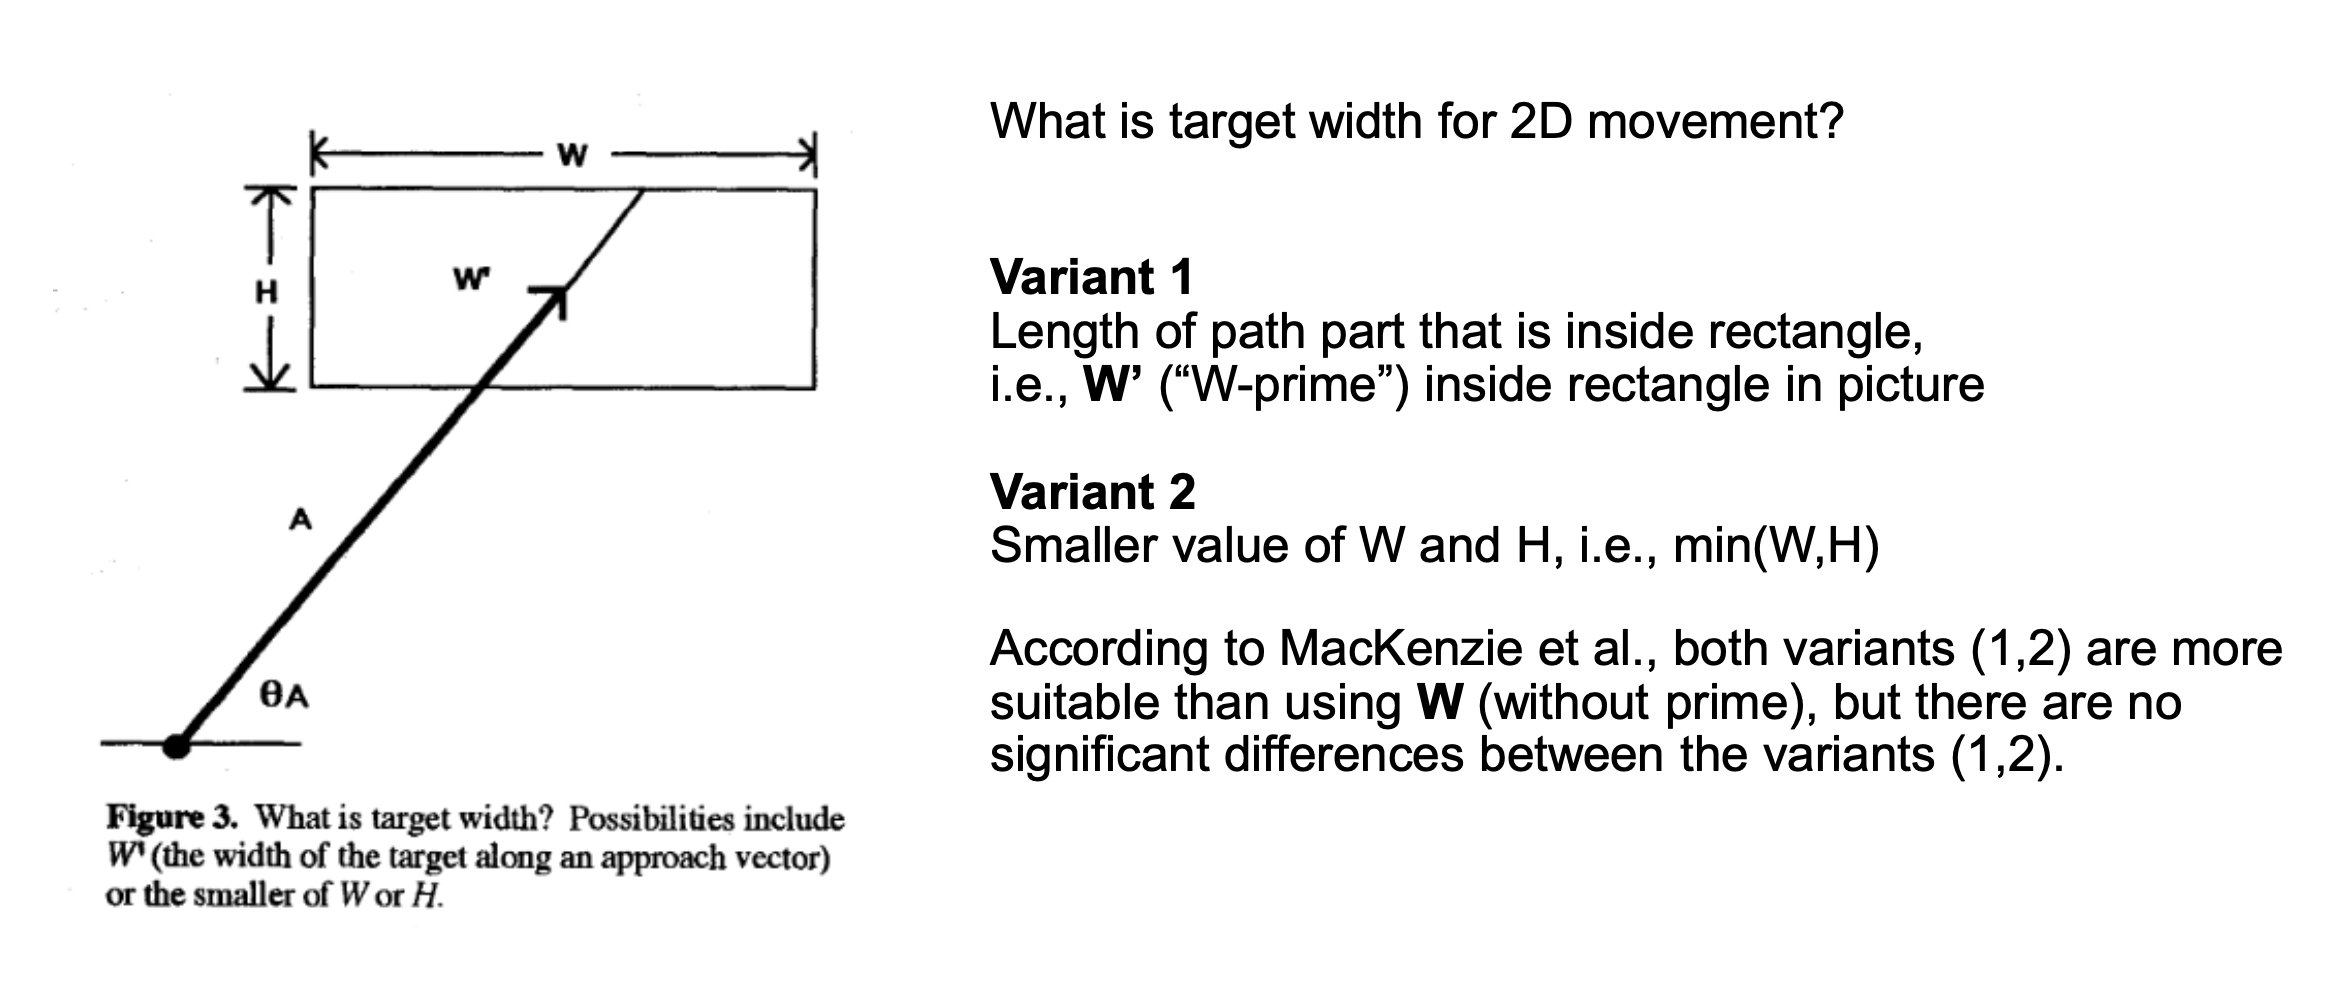
\includegraphics[width=\linewidth]{fitts_law_2d_2.png}
\end{center}

\textbf{Properties} \smallskip

\textit{Direct / indirect input} \smallskip

\begin{itemize}[itemsep=-5pt, topsep=0pt, leftmargin=*]
	\item Direct: Touchscreen, "grasping" virtual 3d objects
	\item Indirect: Mouse movement translated to cursor position (virtual cursor can directly/indirectly manipulate virtual content)
\end{itemize}

\textit{Absolute / relative} \smallskip

\begin{itemize}[itemsep=-5pt, topsep=0pt, leftmargin=*]
	\item Absolute: Position of input mapped to position of output (e.g. drawing tablet)
	\item Relative: Change of input position mapped to change of output position (e.g. mouse)
\end{itemize}


\textit{Position control / rate control} \smallskip


\begin{itemize}[itemsep=-5pt, topsep=0pt, leftmargin=*]
	\item Manipulate position of something (e.g. mouse cursor) versus its velocity (e.g. thumbstick)
\end{itemize} \medskip

\textit{Degrees of freedom} \smallskip

\begin{itemize}[itemsep=-5pt, topsep=0pt, leftmargin=*]
	\item Examples: only 2D position along surface (2 DoF), 3D position and rotatoin in mid-air (6 DoF), or other combination (3D position + rotation around one axis : 4 DoF)
\end{itemize} \medskip

\textit{Isotonic / elastic / isometric} \smallskip

\begin{itemize}[itemsep=-5pt, topsep=0pt, leftmargin=*]
	\item Movable (isotonic e.g. mouse) vs. movable but goes back to neutral position (elastic, e.g. joystick) vs. immovable (isometric, sense force only e.g. lenovo red dot)
\end{itemize} \medskip

\textbf{Performance/Bandwidth} \smallskip

The performance depends on the human (bandwidth of muscle groups connected to input device), the device (effective bandwidth of input device) 
and application (precision requirements of the task). \medskip

\textbf{Effectiveness} \smallskip

\begin{multicols}{2}
    \begin{itemize}[itemsep=-5pt, topsep=0pt, leftmargin=*]
	\item Pointing speed
	\item Pointing precision
	\item errors
	\item Time to learn
	\item Time to grasp device
	\item User preference
	\item Desk footprint
	\item Cost
	\end{itemize}
\end{multicols}


\textbf{Design Space by Card et al} \smallskip

Input device as six-tuple: (M, In, S, R, Out, W) \smallskip

\begin{multicols}{2}
    \begin{itemize}[itemsep=-5pt, topsep=0pt, leftmargin=*]
	\item M: Manipulation operator
	\item In: Input Domain
	\item S: Current state of device
	\item R: (Resolution) Mapping from input domain to output domain
	\item Out: Output domain
	\item W: Additional aspects of ow device works (input lag etc.)
	\end{itemize}
\end{multicols}


\begin{center}
	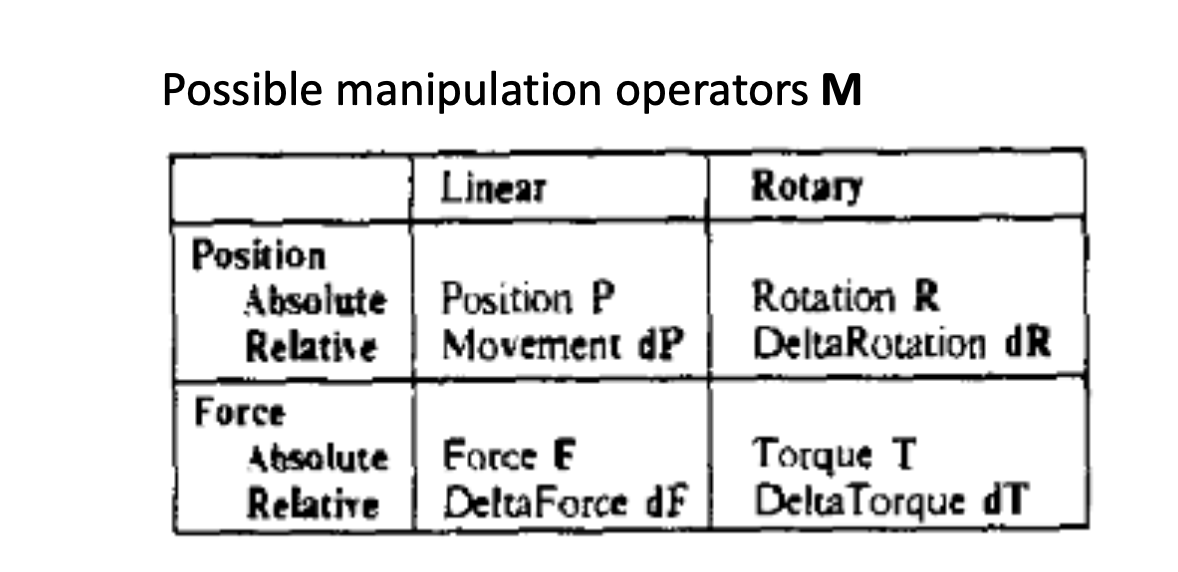
\includegraphics[width=\linewidth]{manipulation_operators.png}
\end{center}

\textbf{Composition operators} \smallskip

\begin{itemize}[itemsep=-5pt, topsep=0pt, leftmargin=*]
	\item Merge composition: e.g. sensed X-Y movement of mouse merged into 2D input
	\item Layout composition: Seperate independent inputs on a device (e.g. independent buttons or wheels on mouse)
	\item Connect composition: Output of one device/sensor mapped into input of another (e.g. physical mouse is input for virtual screen cursor). In this context virtual cursors count also as input devices. 
\end{itemize}

\textbf{Card's Graphical representation} \smallskip


\begin{center}
	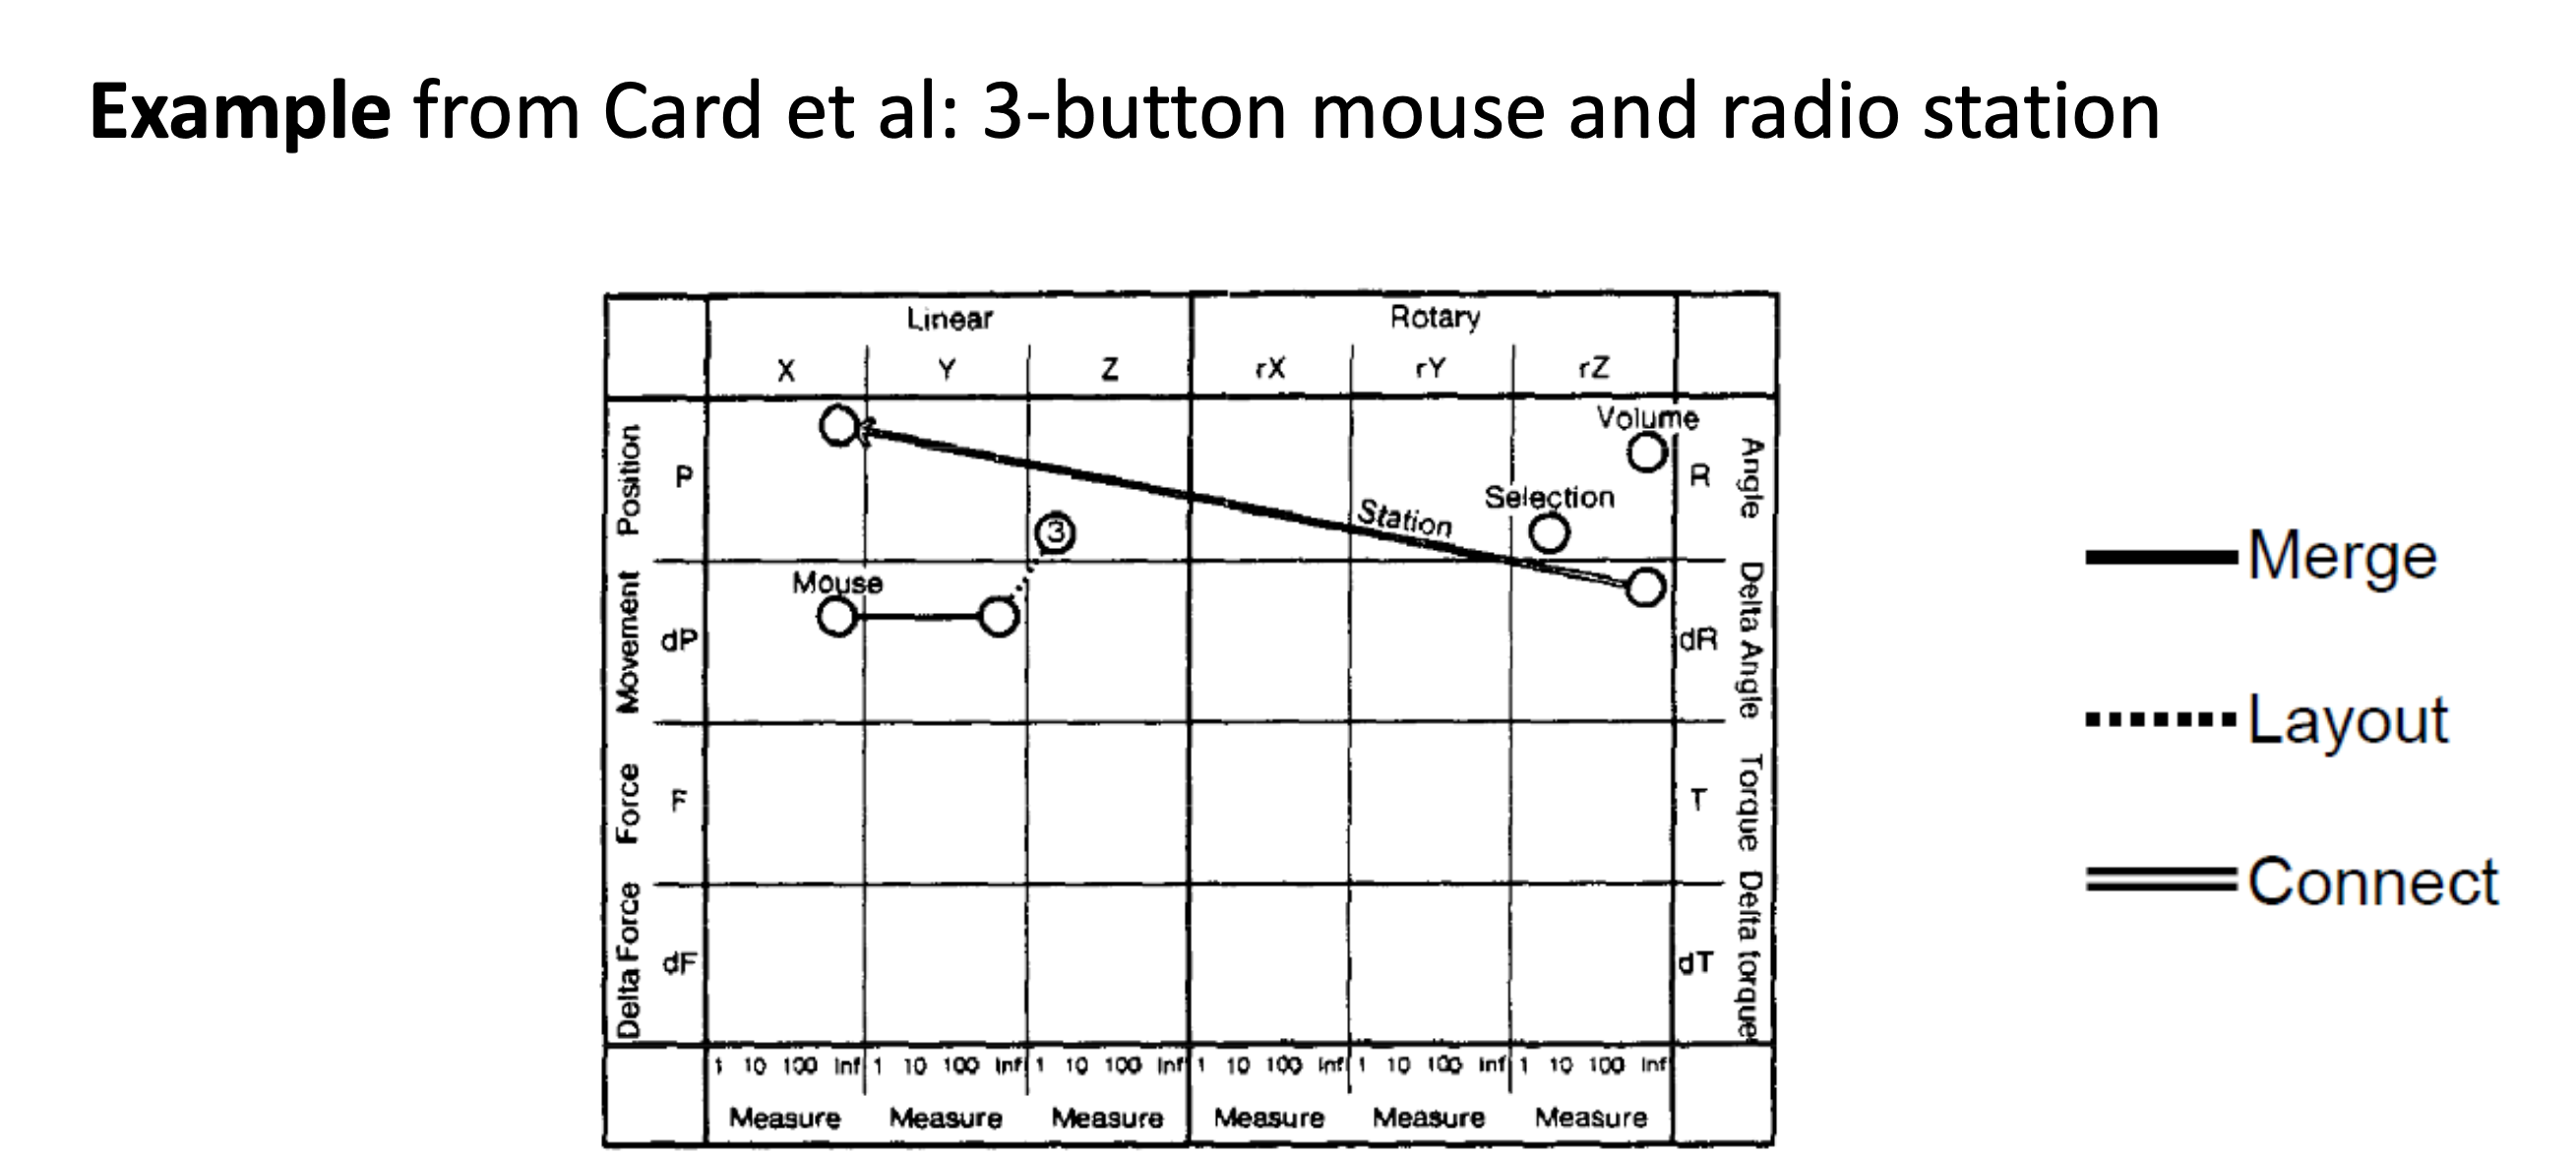
\includegraphics[width=\linewidth]{card_graphical_representation.png}
\end{center}


\textbf{Input Decoding} \smallskip

\textit{Touch Input} \smallskip

Issues with touch: It's noisy and touch area larger than the target. Also visual occlusions. Mobility increaases accuracy issues. 

\begin{center}
	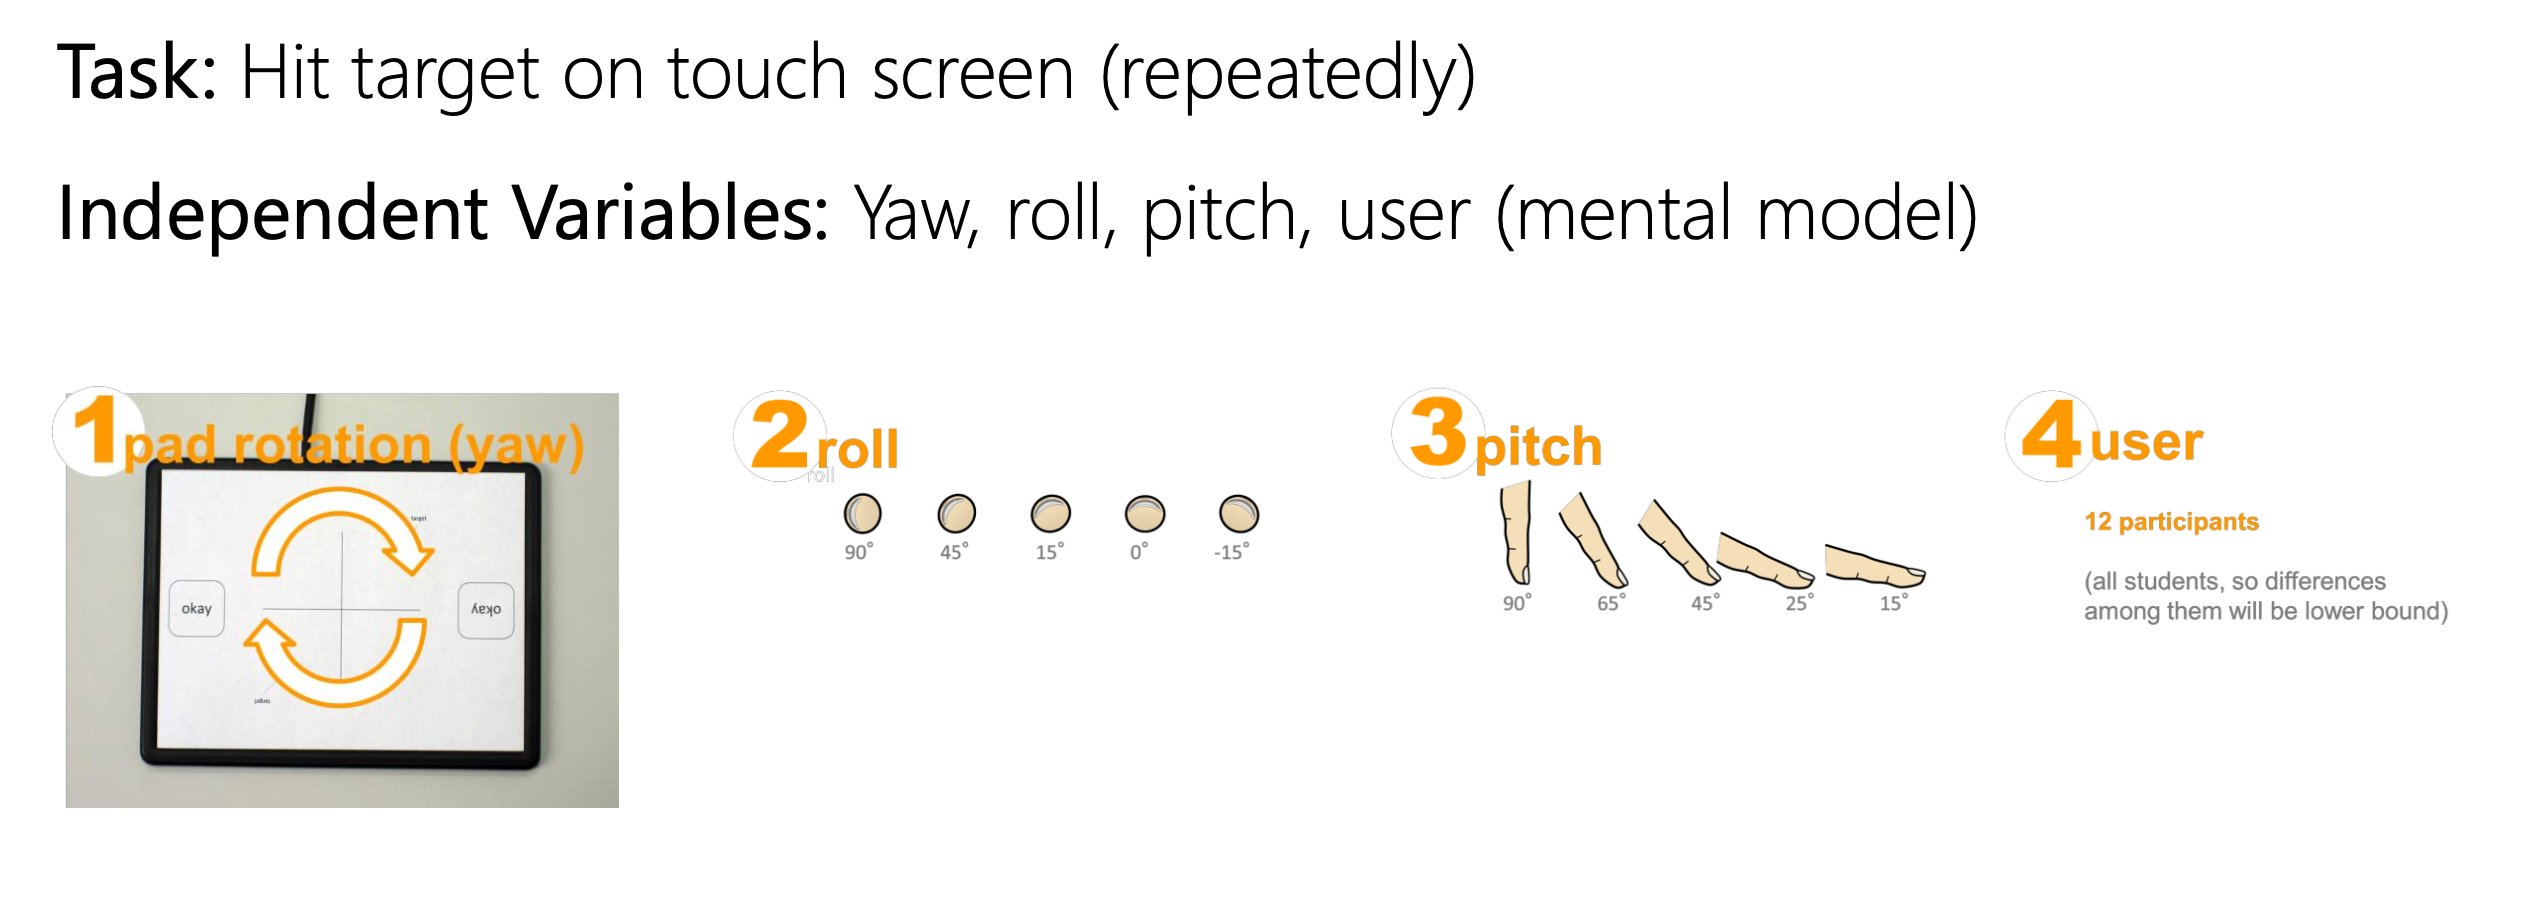
\includegraphics[width=\linewidth]{touch_experiment.png}
\end{center}

We record every trial as a dot at the touch location. Without influence of independent variables should result in circles. If the locations fall into clusters we can compensate if condition is know. \medskip

\textit{Minimum Touch Input Size}

\begin{center}
	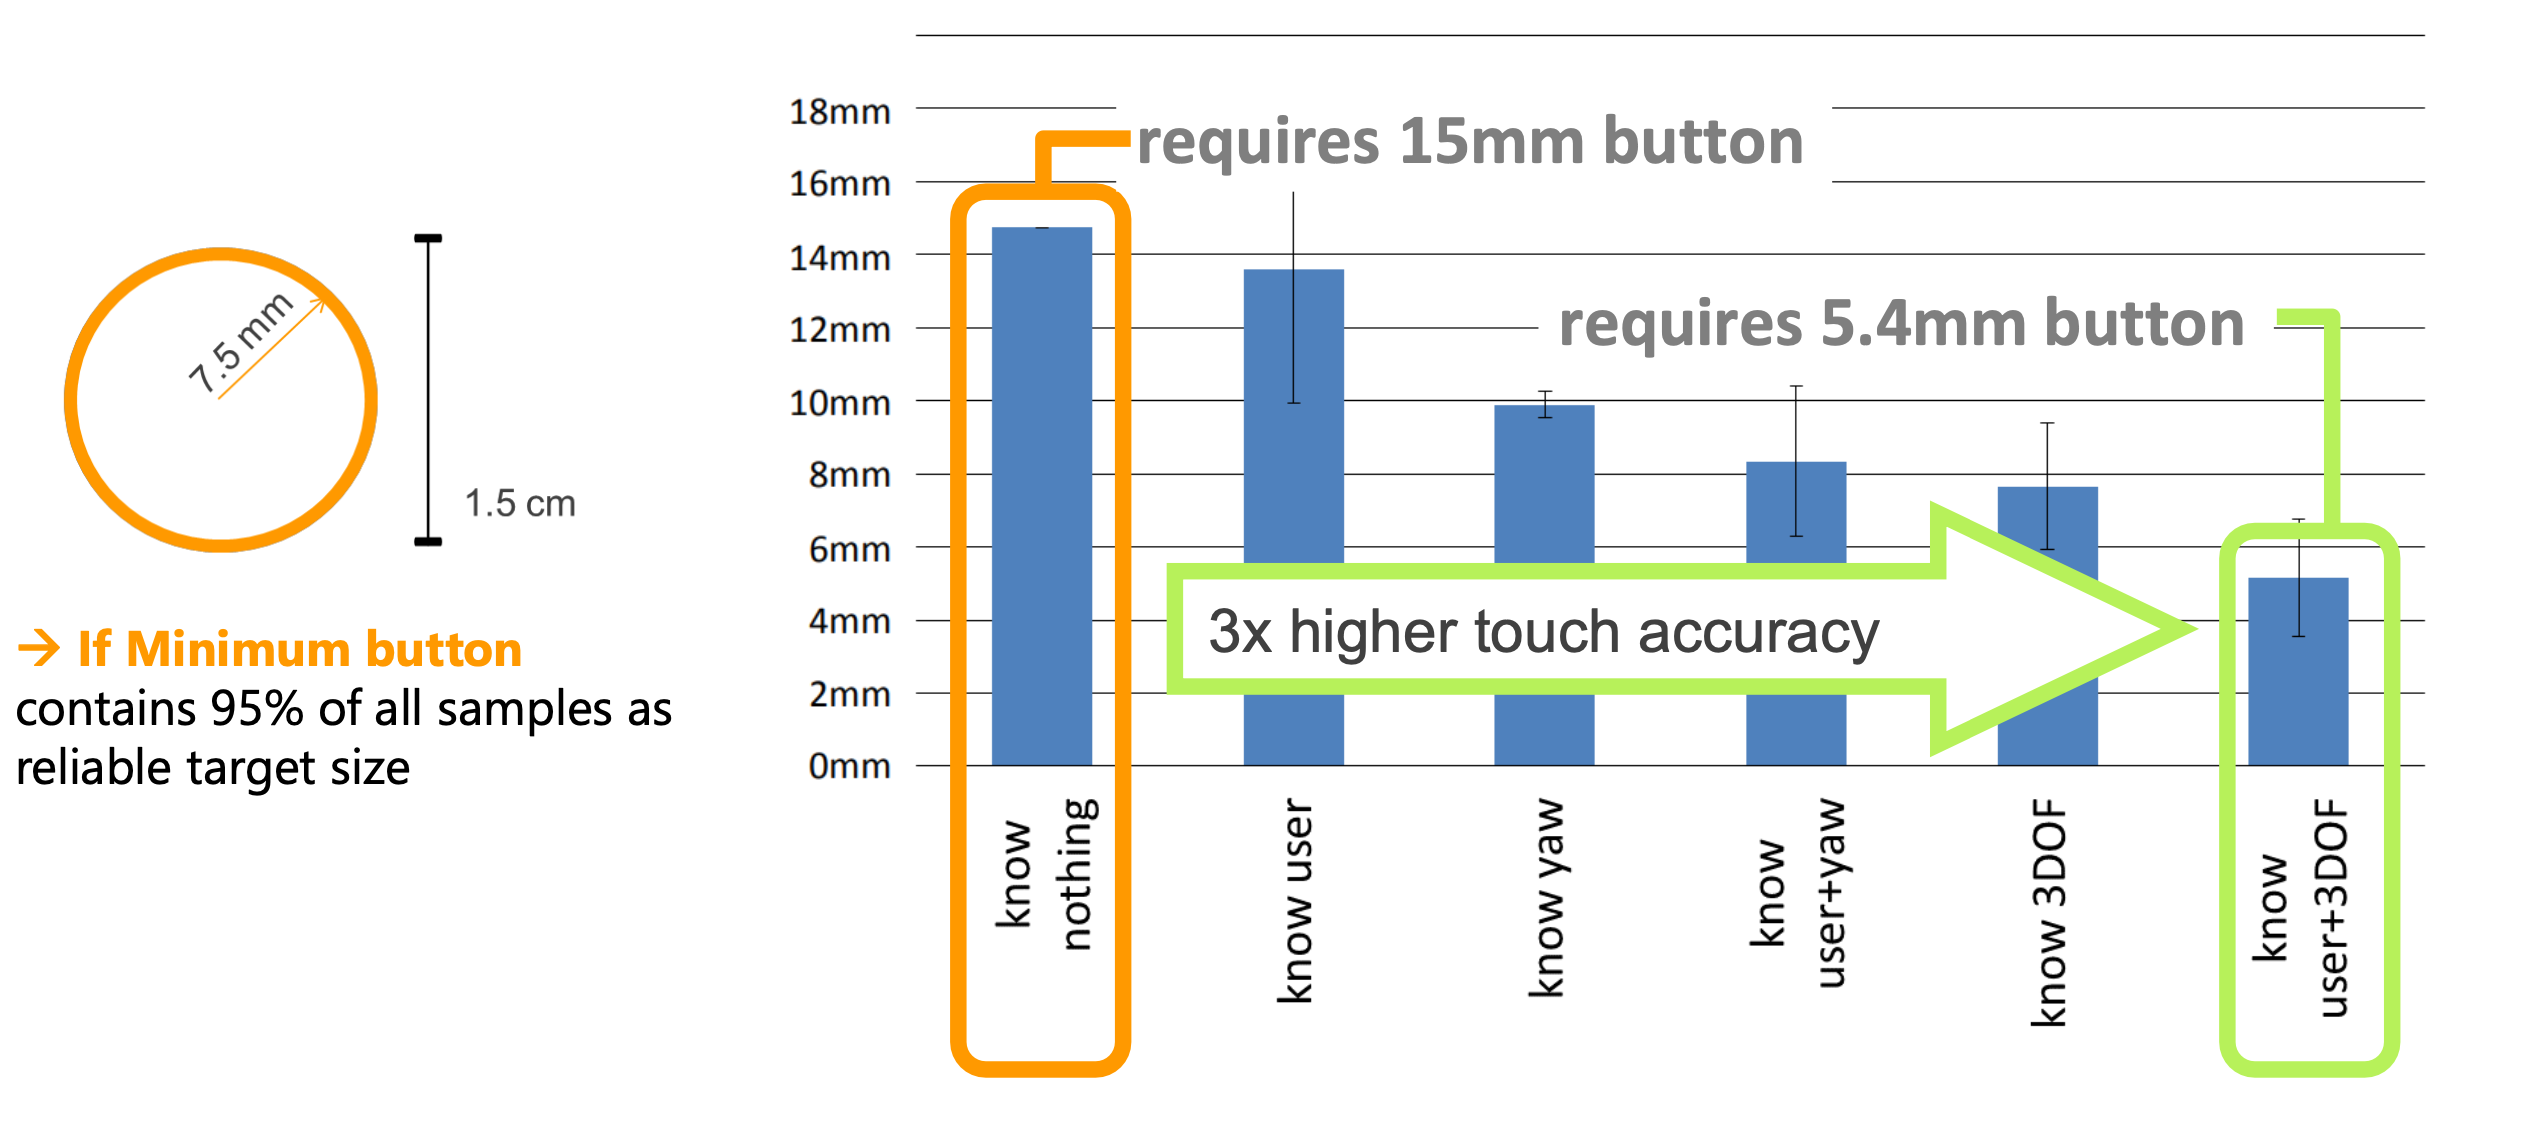
\includegraphics[width=\linewidth]{button_size.png}
\end{center}

\textit{Representing Input} \smallskip


\begin{center}
	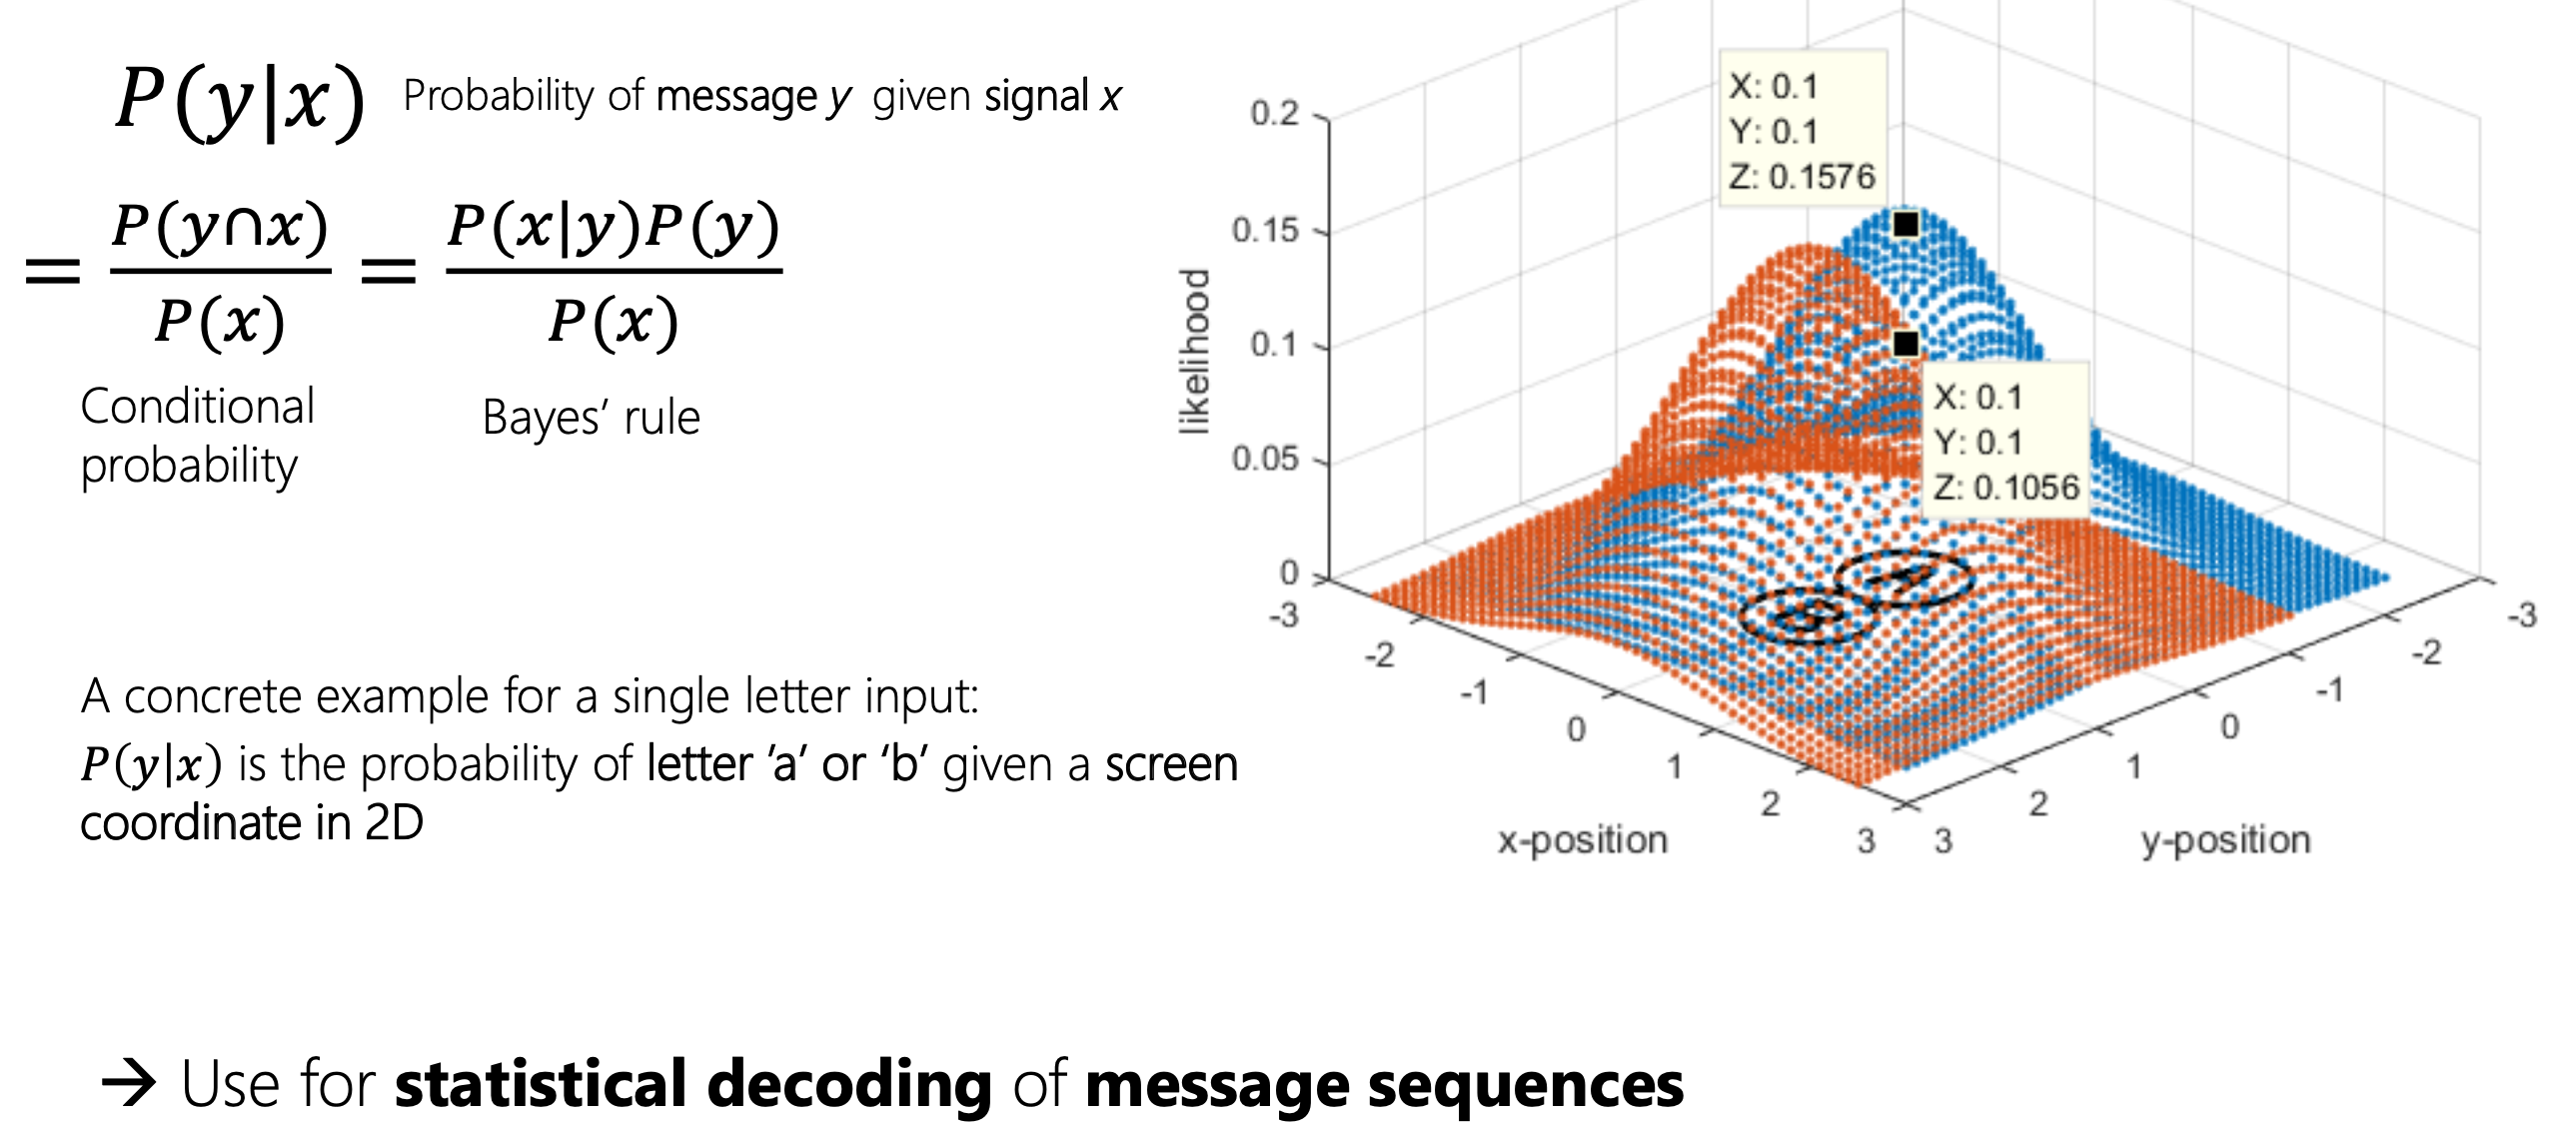
\includegraphics[width=\linewidth]{representing_input.png}
\end{center}

\textit{Sequence decoding} \smallskip

\begin{center}
	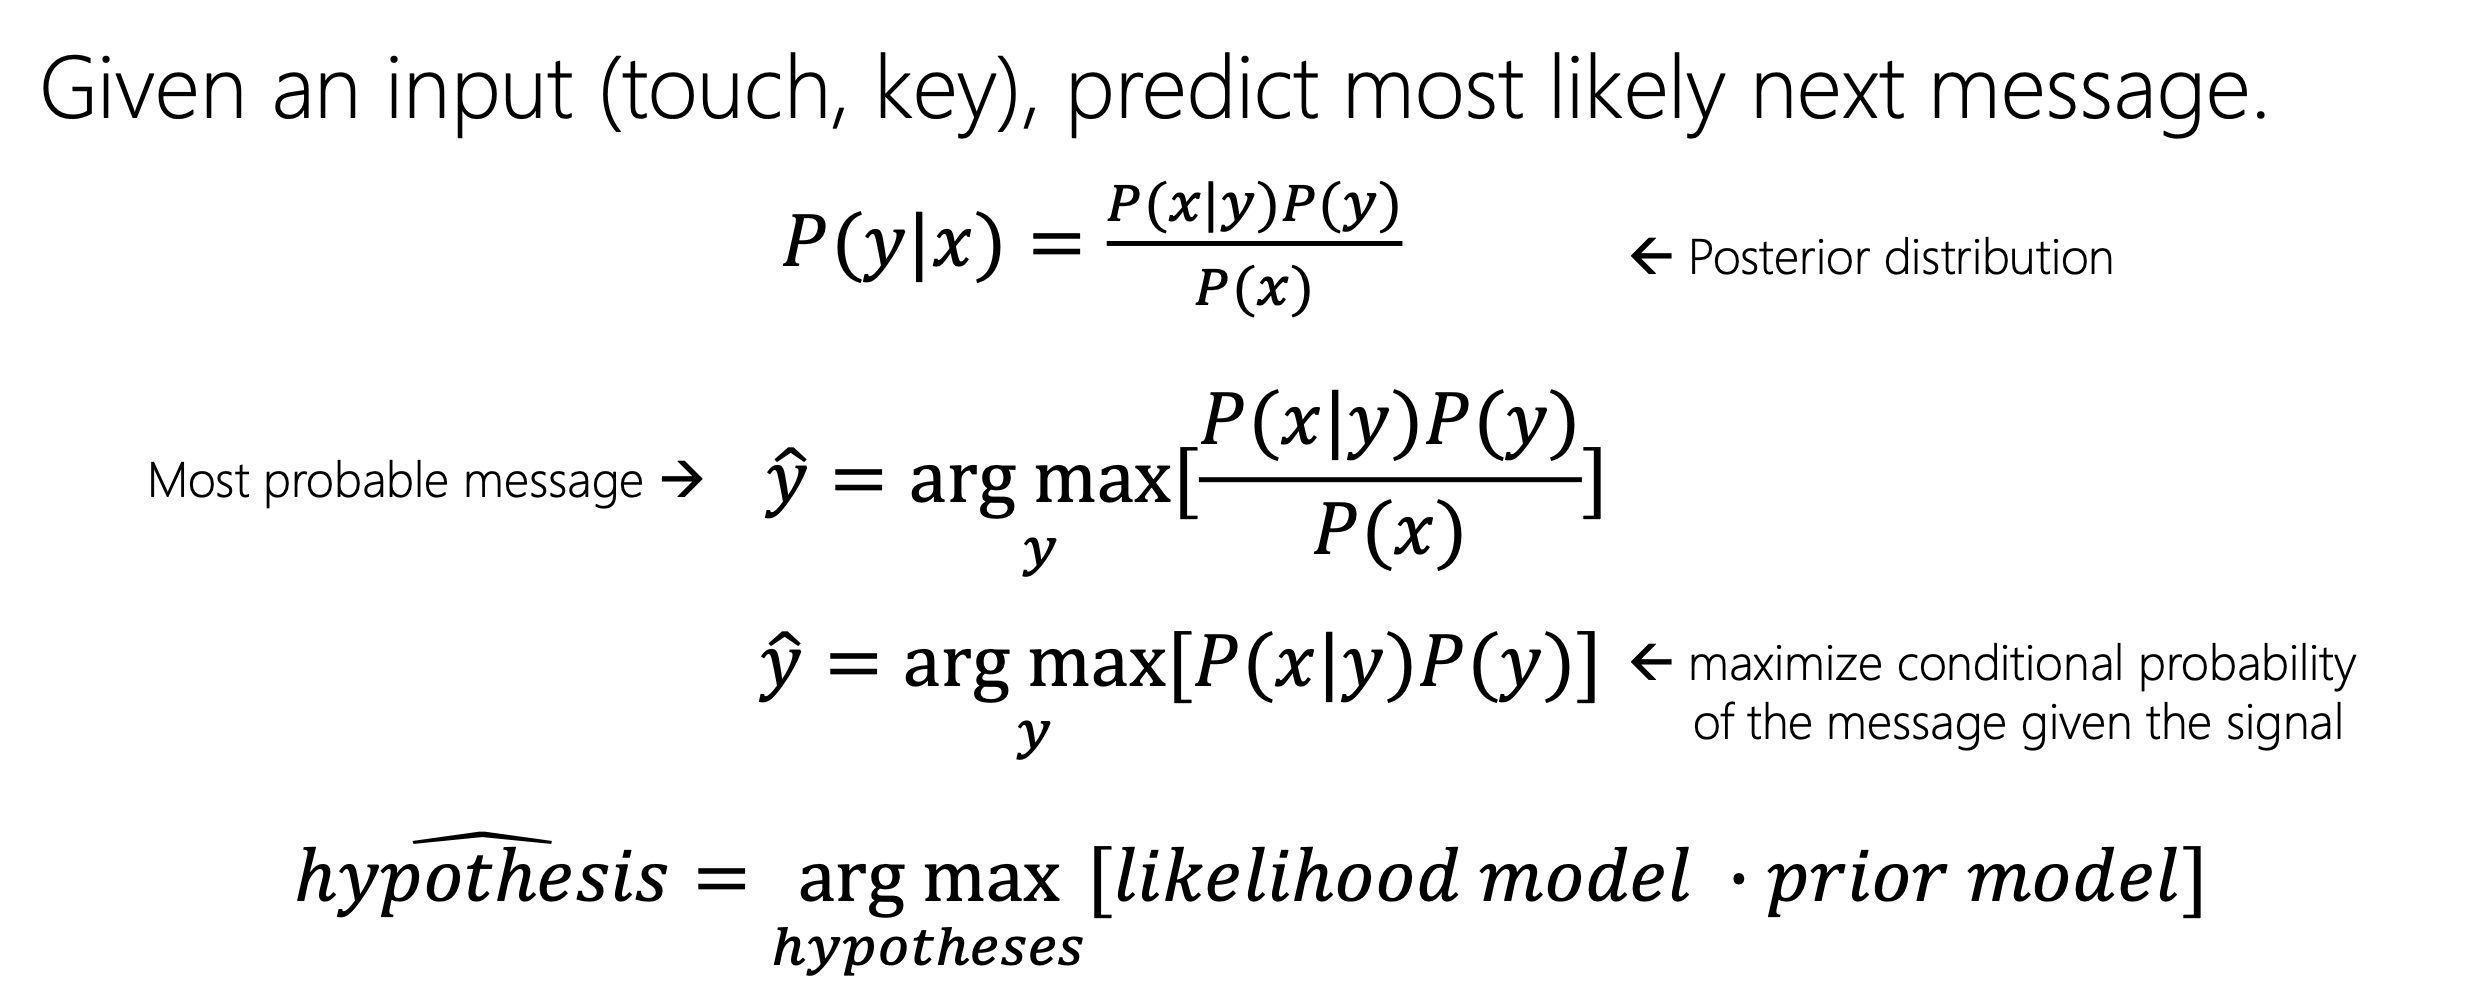
\includegraphics[width=\linewidth]{sequence_decoding.png}
\end{center}

An example would be to investigate noisy sequences of input and identify the most likely sequence of intended presses.
Observation would be the 2D screen coordinates of tap and the observation sequence are the time-ordered observations. 
\smallskip

A token in this context would be a datastructure containing the accumulated probability of hypothesis. 
$$Acc\_Prop_{n+1} = Acc\_Prob_{n} * prior * likelihood$$


\textit{Simple sequence decoding} \smallskip

One token per hypothesis per obervation. 


\begin{center}
	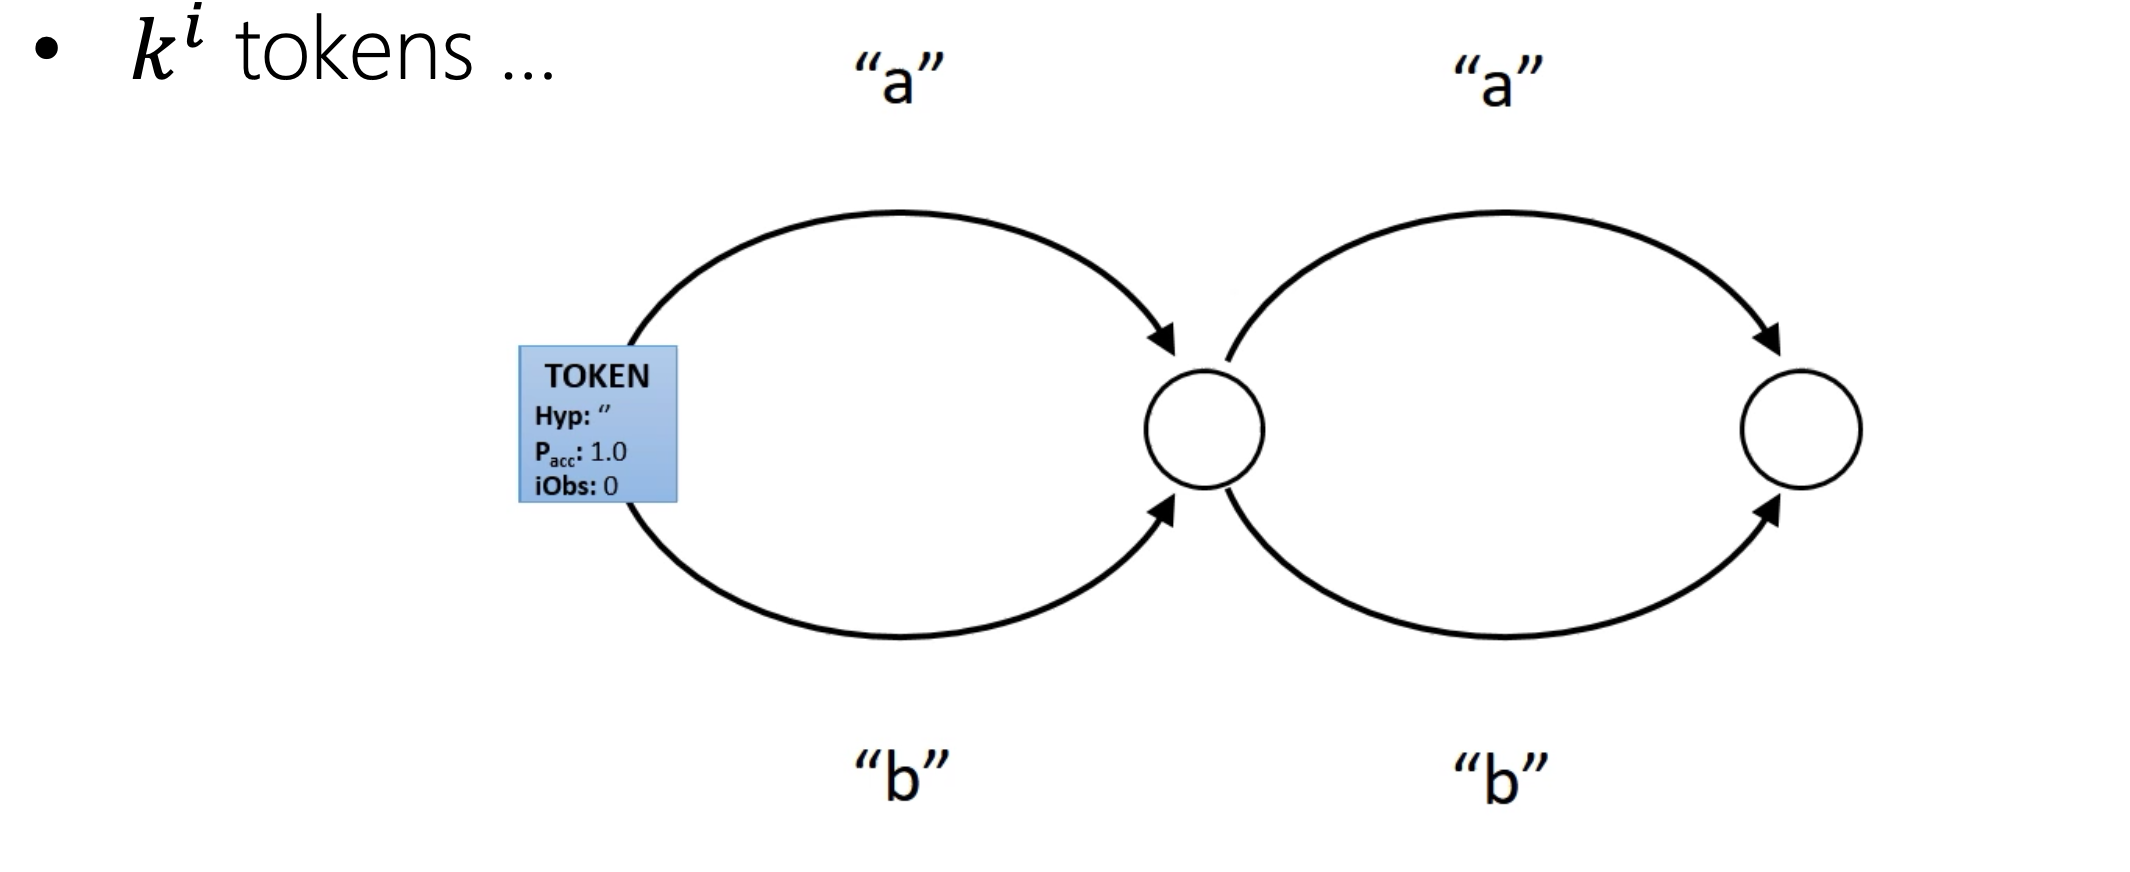
\includegraphics[width=\linewidth]{simple_sequence_decoding.png}
\end{center}


\textit{Substitution-only decoder} \smallskip

\begin{center}
	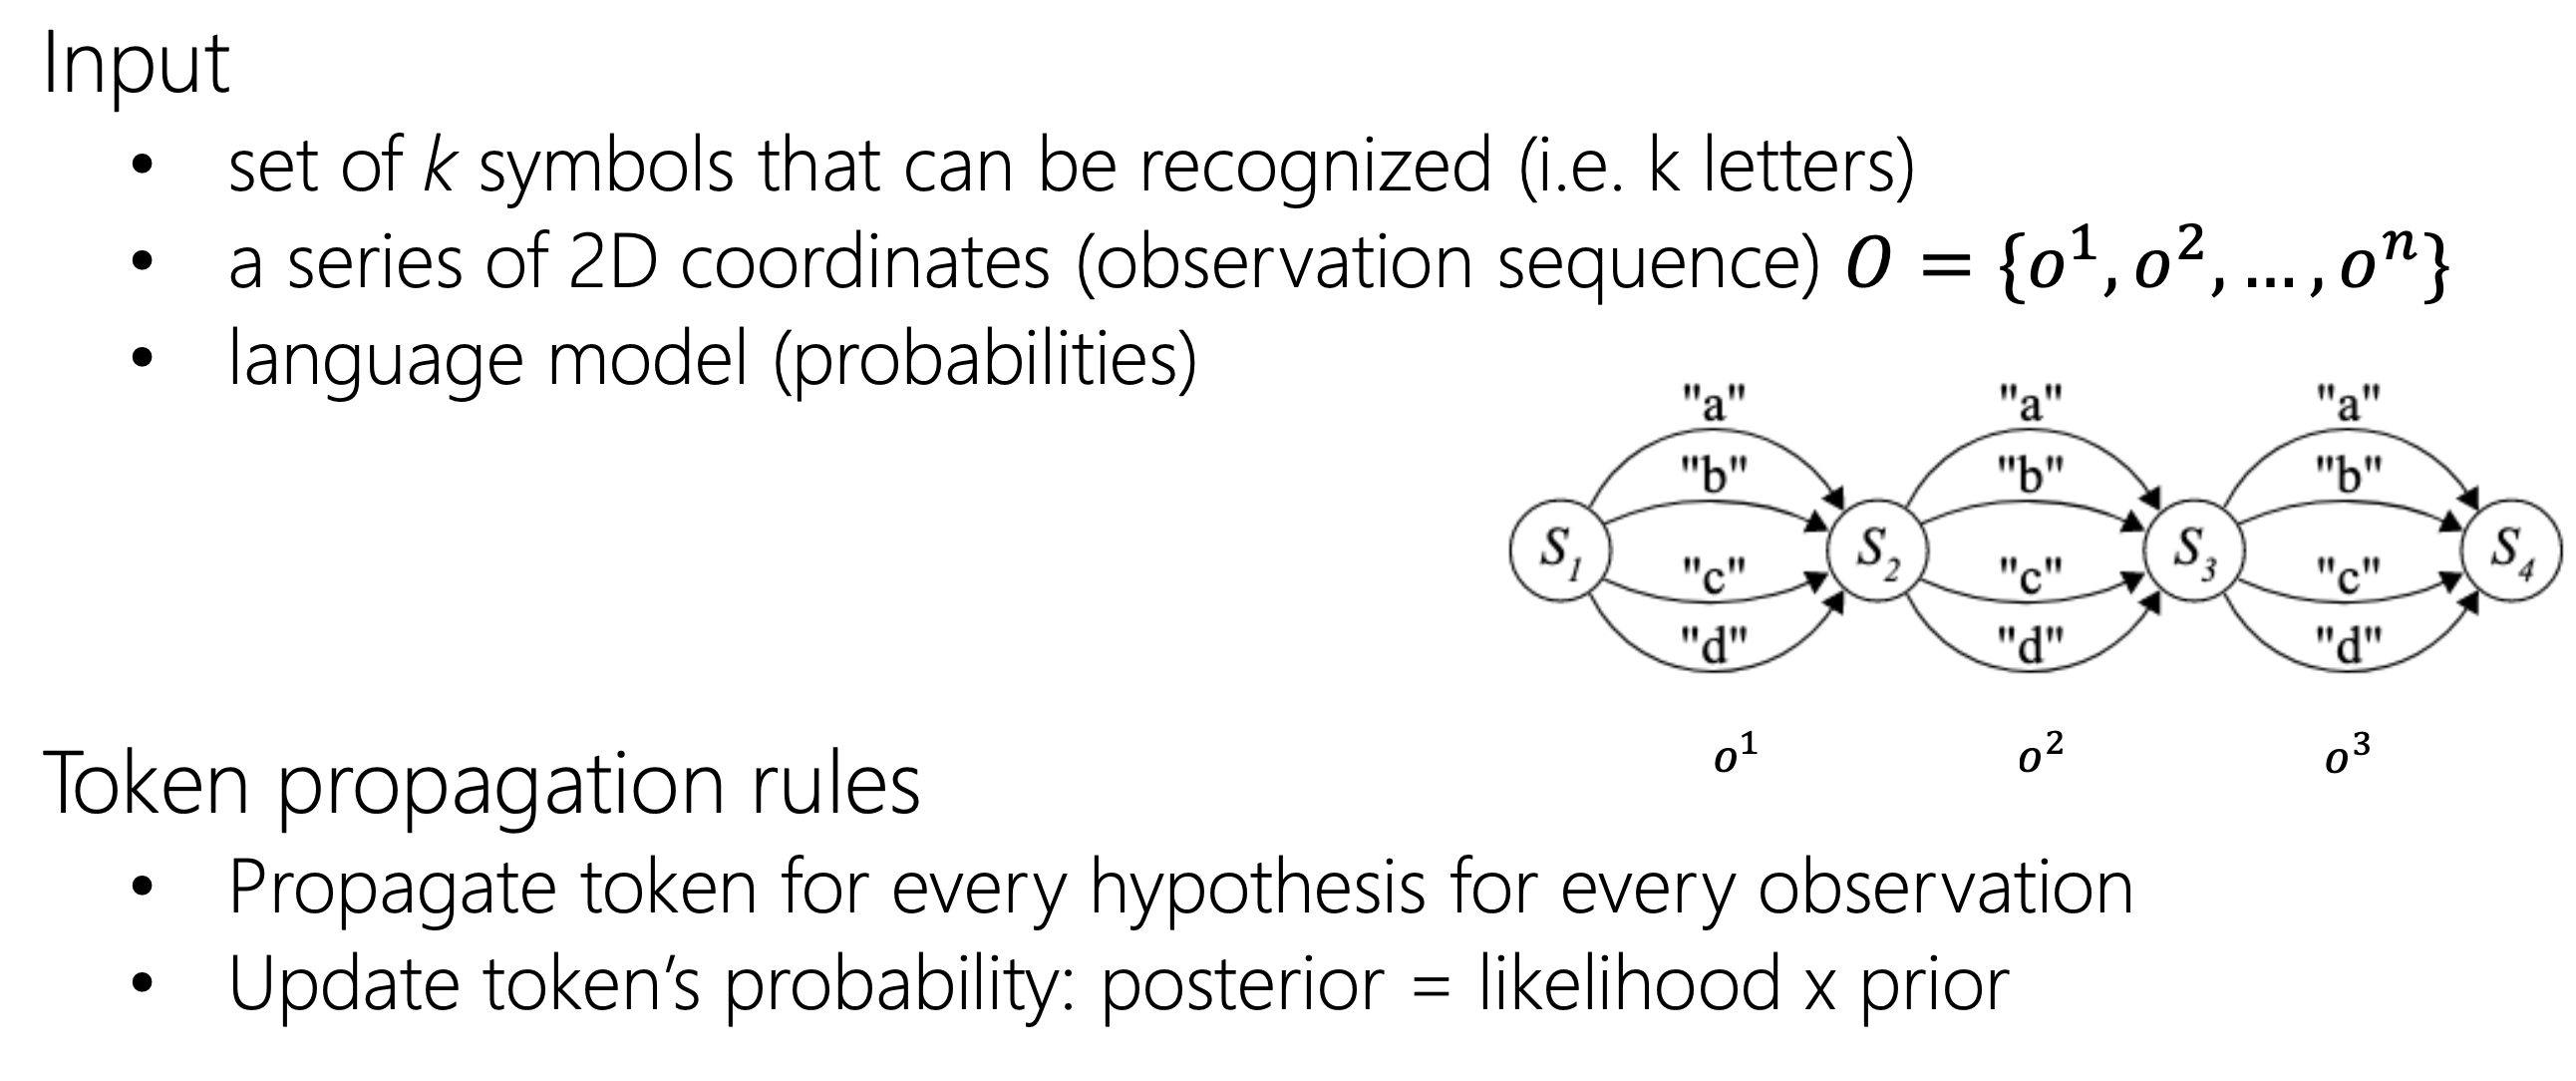
\includegraphics[width=\linewidth]{substitution_only_decoder.png}
\end{center}

\textit{Bream Pruning} \smallskip

we have an infinite search space but only a few plausible hypothesis. We prevent propagation of unlikely tokens. 

Rules of beam Pruning: 

\begin{itemize}[itemsep=-5pt, topsep=0pt, leftmargin=*]
	\item Only propagate a token if its probability is among the n-best probs for the observation so far 
	\item If the new prob of the observation is among the n-best then update the list of tokens to propagate
\end{itemize}

Threshold is also known as beam size. 

\begin{center}
	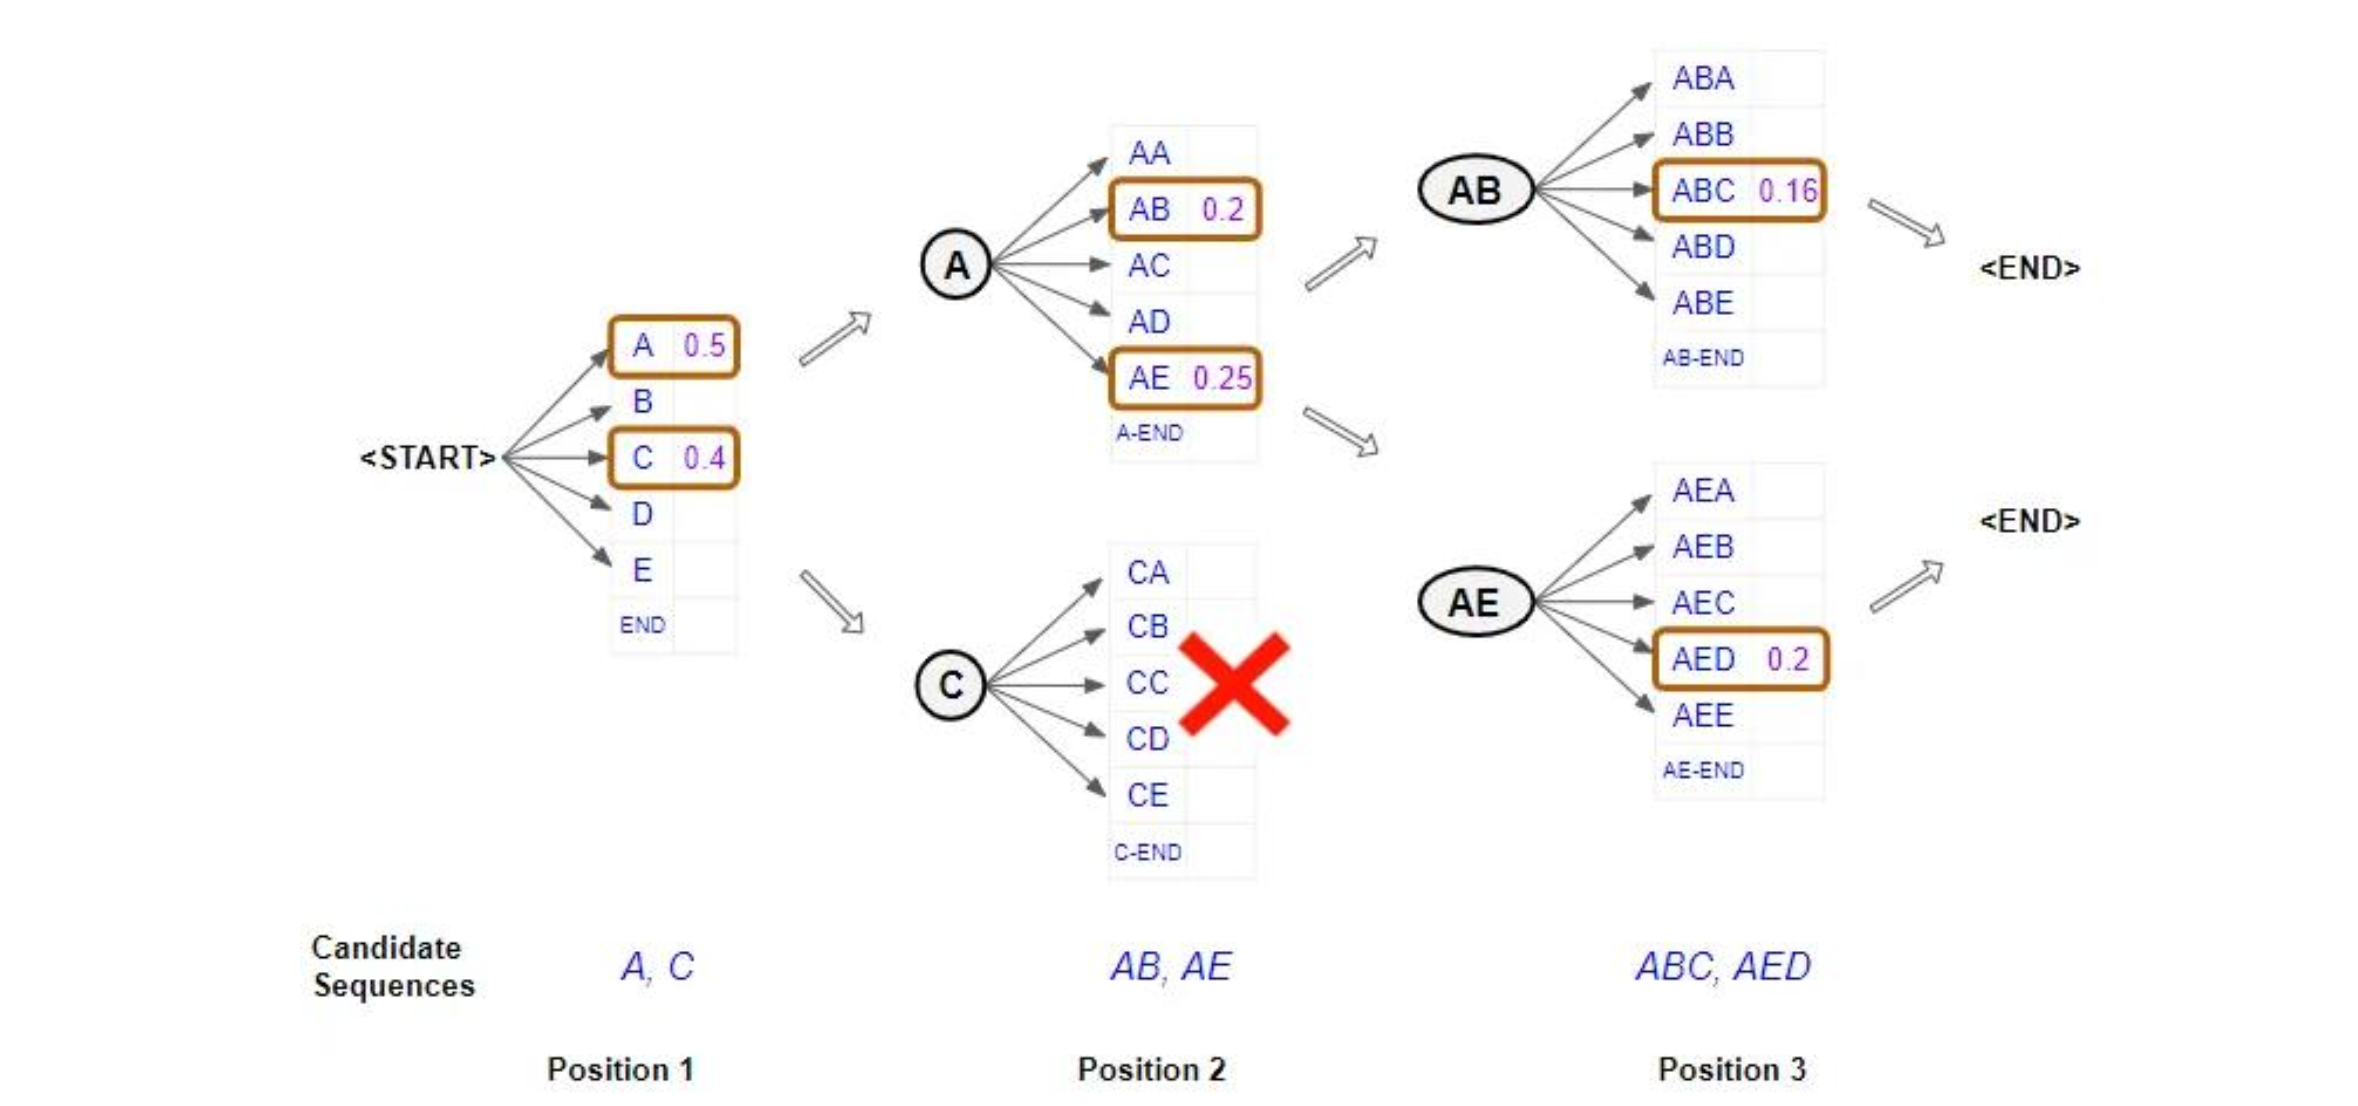
\includegraphics[width=\linewidth]{beam_pruning.png}
\end{center}

\textit{Language models} \medskip

Probabilities for the decoder come from Language models. Language models are the probability of individual words or word sequences. 
A vast amount of letter combinations is unlikely to be written. These models capture valid letter and word sequences and assign them probabilities. 
These probabilities can be leveraged to infer or predict what users want to write, based on what they have already written. \medskip

The simplest models are uni- or bigrams. (Unigram contains one token only and bigrams obviously two). \medskip

\textit{Trigram Model}

\begin{center}
	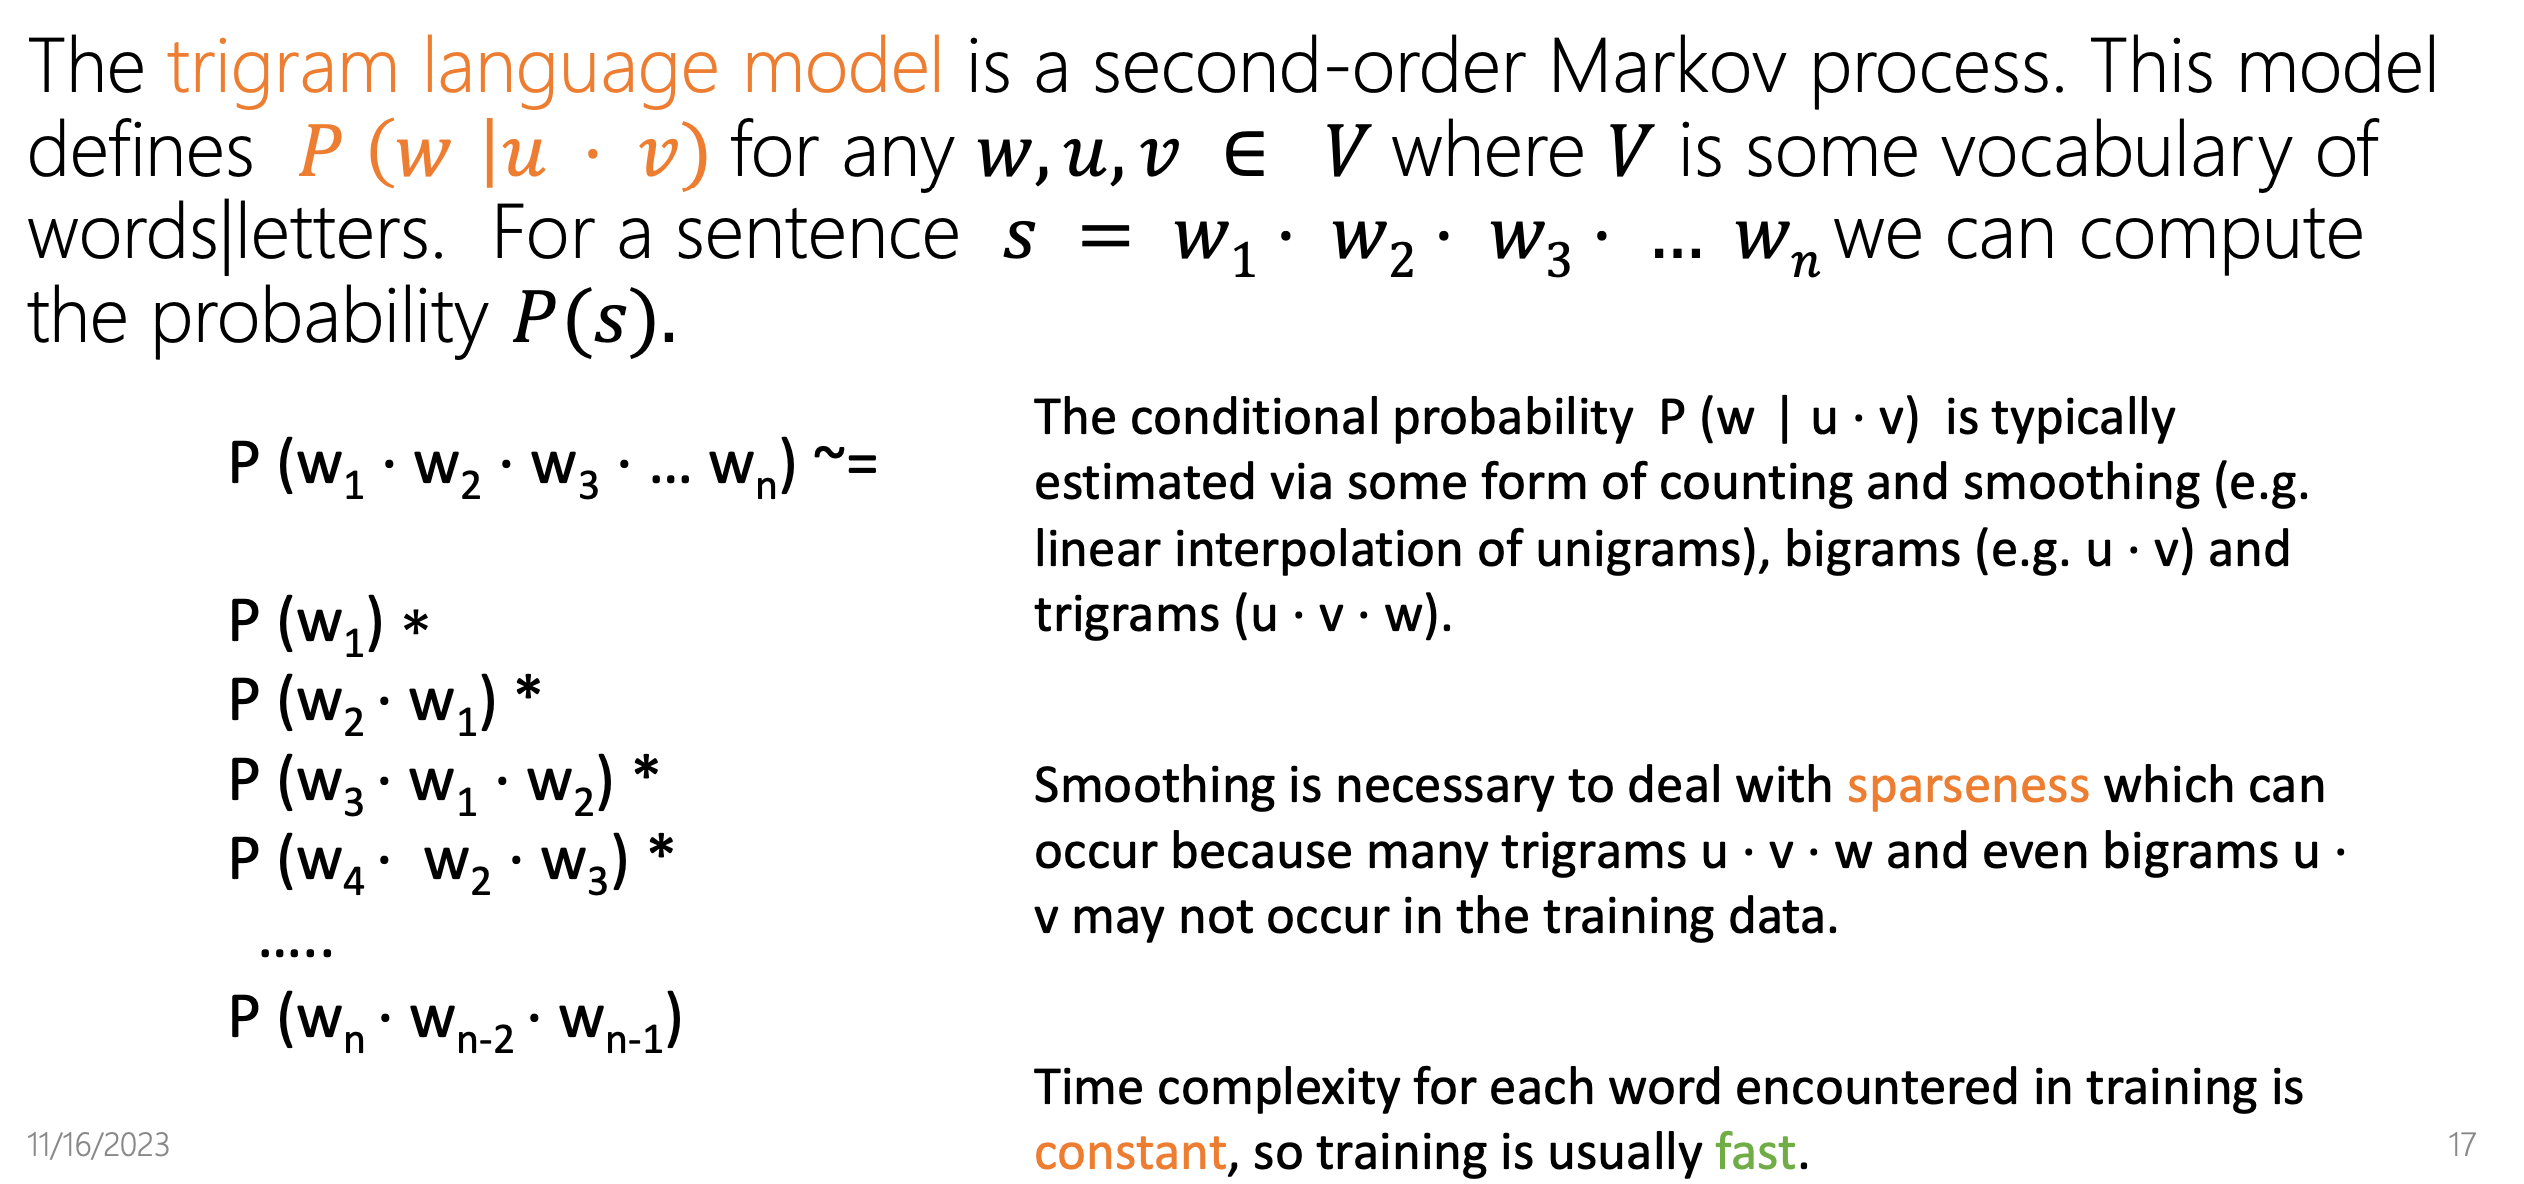
\includegraphics[width=\linewidth]{trigram_model.png}
\end{center}

\textit{Trigram Model Example}

\begin{center}
	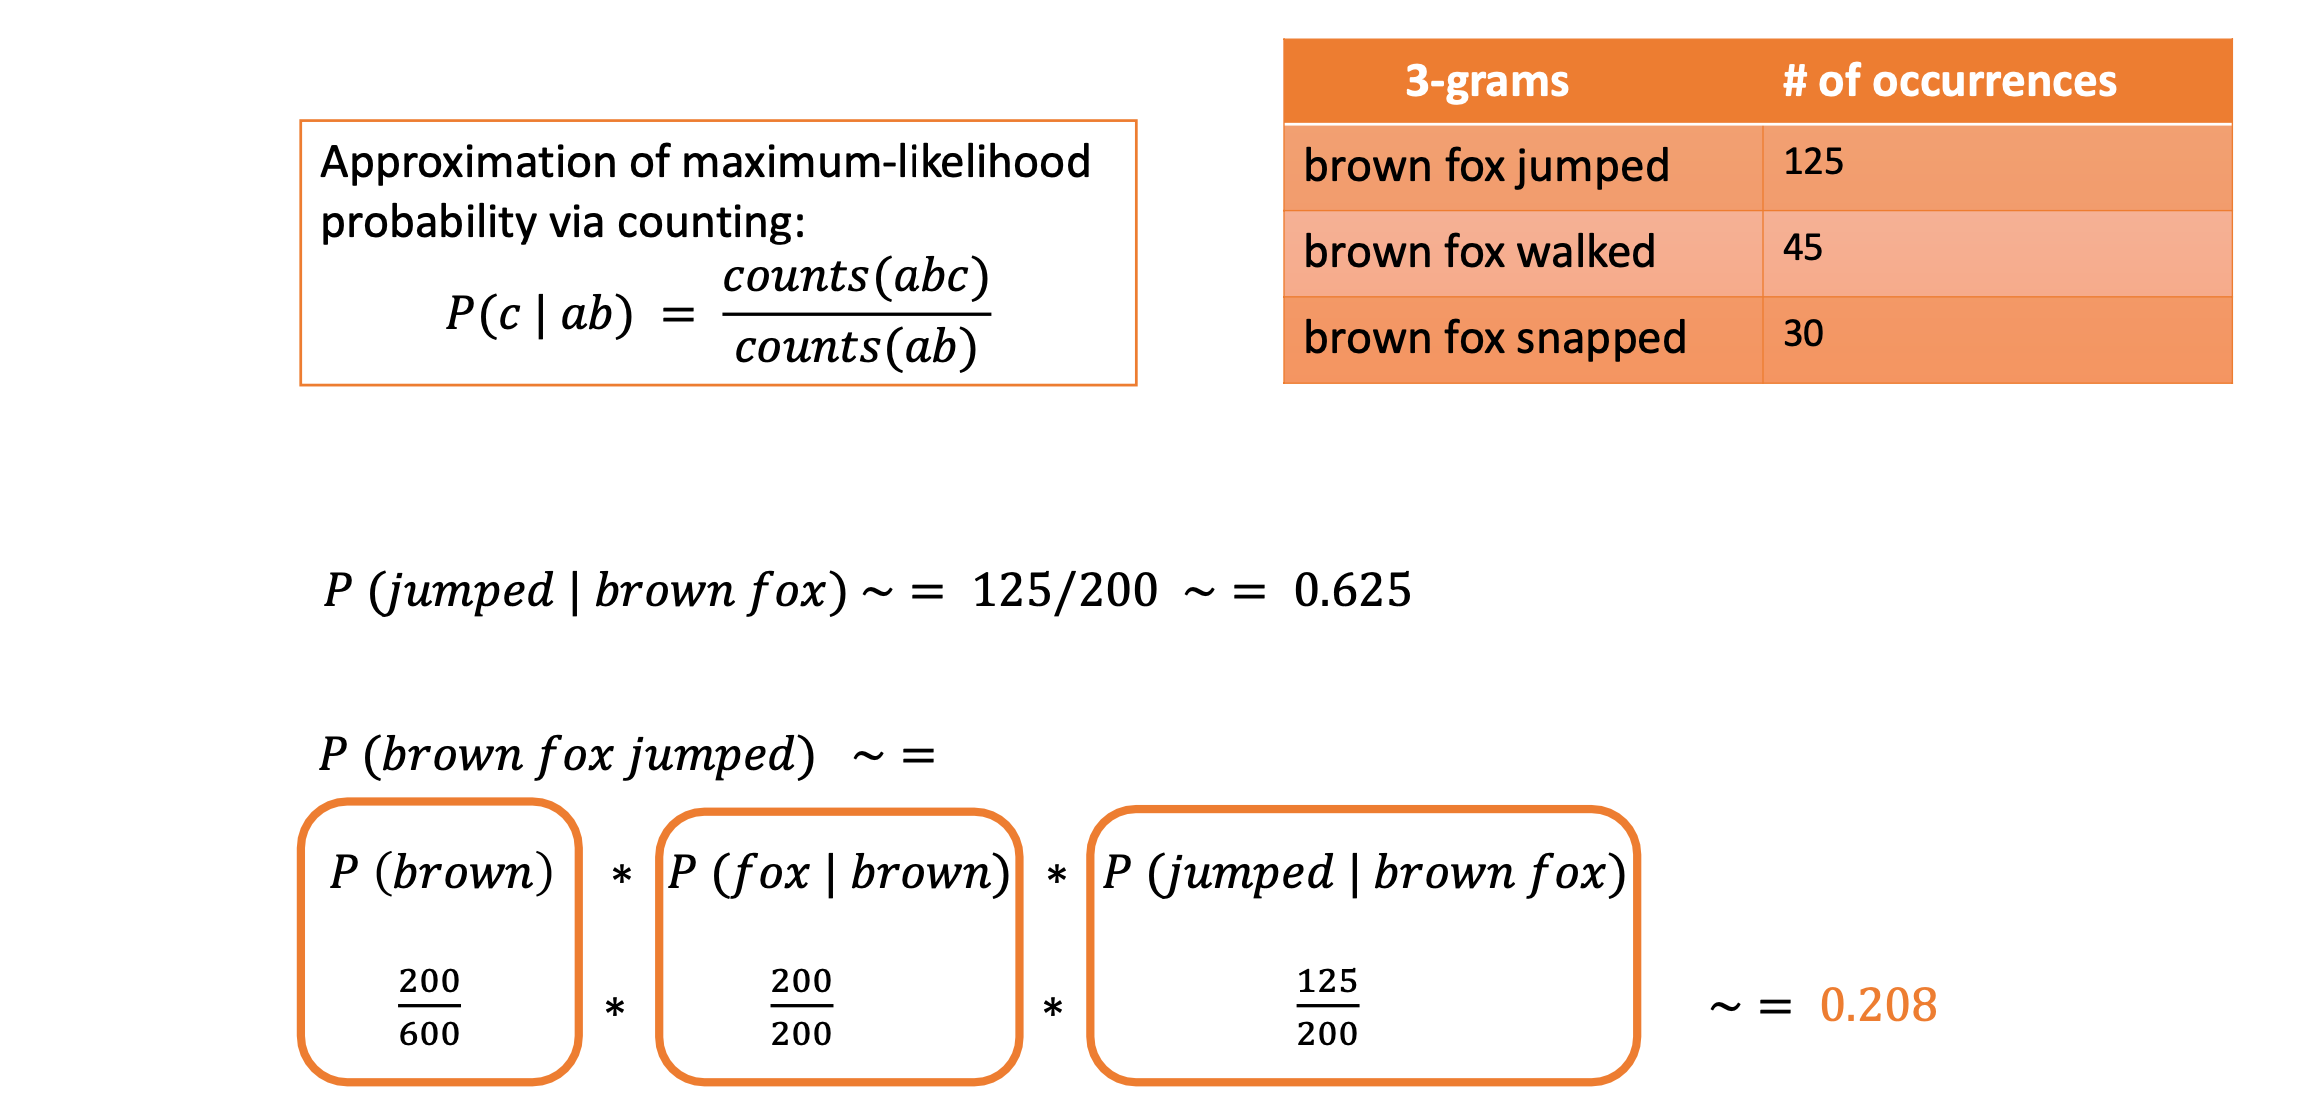
\includegraphics[width=\linewidth]{trigram_model_example.png}
\end{center}

\textit{Advanced statistial language models} \smallskip

Recurrent neural network (RNN) and Generative Pre-trained Transformers(GPT) are able to capture more complex relationsships for many to many token mappings. 

\medskip

We can then combine probabilities from the touch model with a language model to get the most likely key for a touch. 


\begin{center}
	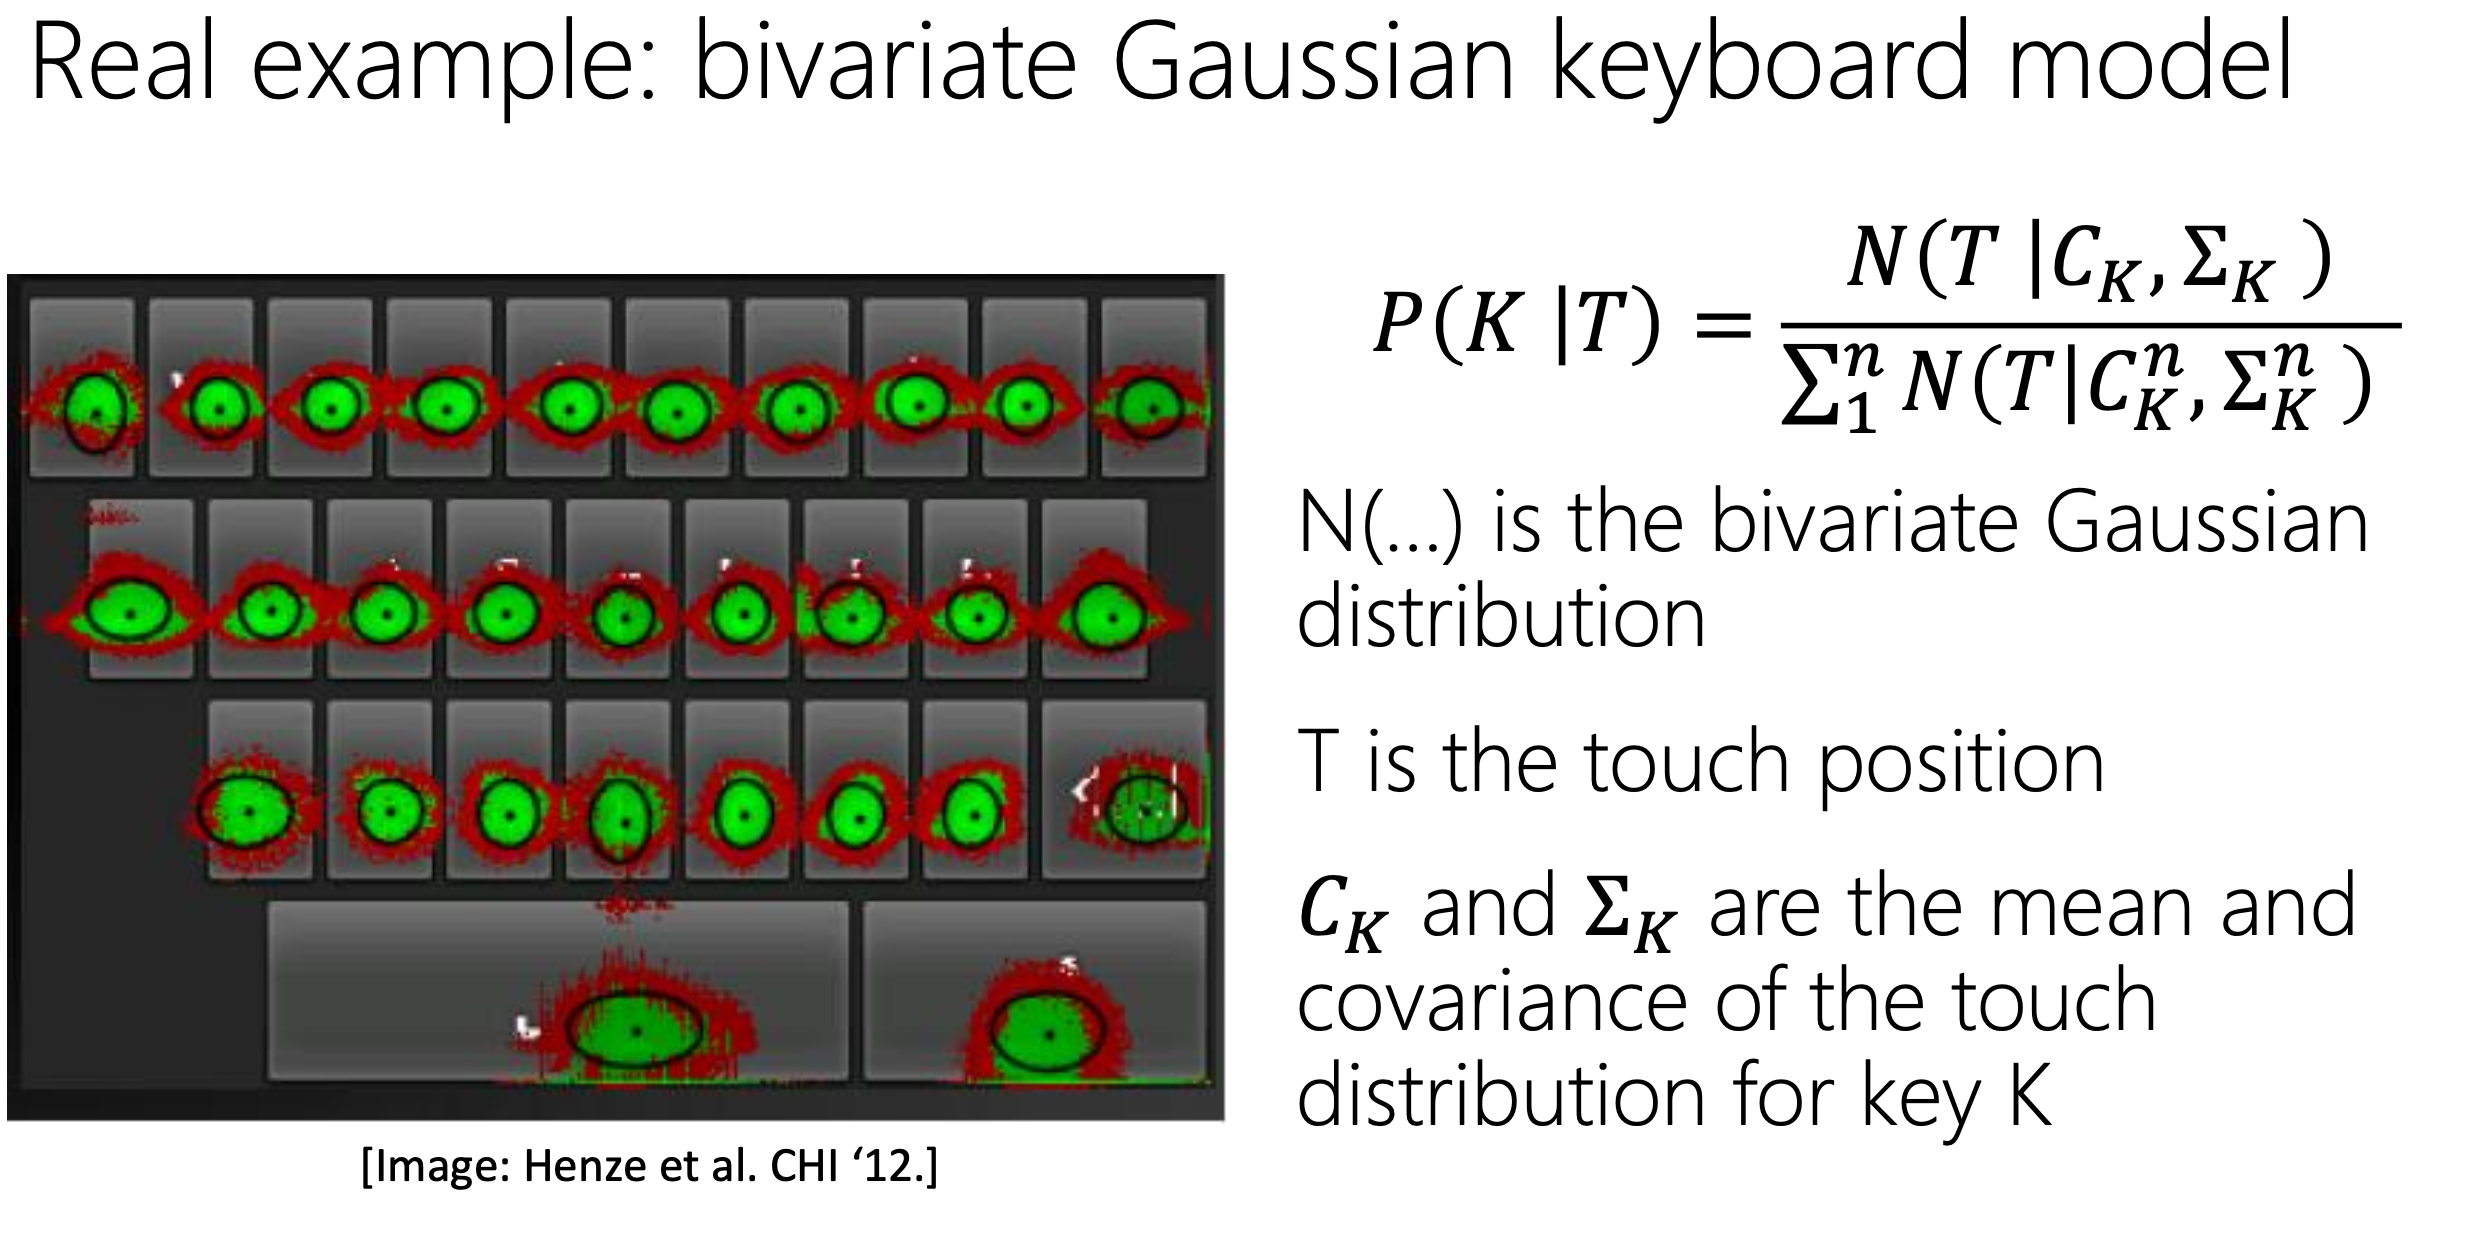
\includegraphics[width=\linewidth]{bivariate_gaussian_keyboard.png}
\end{center}

\textit{Application Examples} \smallskip

\begin{itemize}[itemsep=-5pt, topsep=0pt, leftmargin=*]
	\item Predictive text input
	\item Text input beyond screens
	\item Accessible mixed reality
\end{itemize}

(Check slides if you want to see more on these).



\section{Computational Design}

The main idea of this chapter is to use models and algorithms to help design and optimize interfaces. The chapter will contain: 

\begin{itemize}[itemsep=-5pt, topsep=0pt, leftmargin=*]
	\item Modeling task as combinatorial optimization problem
	\item User models as cost / goodness functions in optimization
	\item The assignment proble and applications in HCI
	\item Exampels
\end{itemize}

Example: 50 different items yield 50! options to create menus. 

\smallskip

\textit{To evaluate a menu we can use:} \medskip

Time to move to an element $i$ :
$$t_i = a + b \log_2 \left( \frac{A_i}{W_i} + 1 \right)$$
Average time to operate a menu:
$$T = \sum_{i} p_i t_i$$

\textbf{Design as Search}

As a goal we want to find the best design decision for given objectives. \medskip

Some benefits of using algos in design: 


\begin{itemize}[itemsep=-5pt, topsep=0pt, leftmargin=*]
	\item Efficiently search large solution spaces
	\item Systematic, rigorous process
	\item Imporoved quality and reliability
	\item Guarantees for goodness og outcomes
\end{itemize}

We want to find optimal $x \in X$ where $X \in \mathbb{K}^n$ which maximizes $f(x)$. So $X$ is the set of all feasible solutions. \medskip

\textit{Formulate optimization problem}
 \begin{multicols}{2}
    \begin{itemize}[itemsep=-5pt, topsep=0pt, leftmargin=*]
        \item The design space (variables, contraints)
        \item Objective functionality
        \item  Way to solve problem (solver)
    \end{itemize}
 \end{multicols}
    

\textit{Design Space} \smallskip

A combination of all design variables forms the design space. Each variable represents an open decision (usually discrete):

\begin{itemize}[itemsep=-5pt, topsep=0pt, leftmargin=*]
	\item Boolean(e.g. show label)
	\item Integer(e.g. color)
	\item Categorical(e.g. type of element)
	\item Continous(e.g. color value)
\end{itemize}

As not all combinations yield a feasible design we need to introduce constraints. \smallskip

Decision variables: \smallskip

$x_{ik} = 
\begin{cases} 
1, & \text{if command } i \text{ assigned to slot } k \\
0, & \text{otherwise}
\end{cases}$

Design space: \smallskip

$X = \{ \mathbf{x} = (x_{ik}) \mid i,k = 1 \ldots N, x_{ik} \in \{0,1\} \}$ \medskip

\textit{Constraints (feasible space)}: \medskip

$\sum_{k=1}^{n} x_{ik} = 1 \quad \forall i = 1 \ldots N$, where each command is assigned to one slot. 


$\sum_{i=1}^{n} x_{ik} = 1 \quad \forall k = 1 \ldots N$, where each slot is assigned to one command.\medskip

\textit{Objective Function} \medskip

Assign a score the each solution in the design space. Goal is to find the solution that maximizes or minimizes the objective function.
Can be interpreted as quality indicator of UI. \smallskip

We can find an objective function in different ways.

\begin{itemize}[itemsep=-5pt, topsep=0pt, leftmargin=*]
	\item Math model
	\item Machine-learning model
	\item Simulation-based model
	\item Look up tables from empirical data
	\item Heristics, guidelines, best-practices
\end{itemize}

Example: Minimize average selection time (linear assignment problem):

$$\min \sum_{i=1}^{n} \sum_{k=1}^{n} p_{i} \cdot t_{k} \cdot x_{ik}$$
Where $p_i$ is prob of item $i$, $x_{ik}$ the constraints and $t_k$ the time to move to slot k from the top. We call $x_{ik}$ the decision variables. 

\textbf{Optimization Methods}

\textit{Mathematical, Exact Methods} \smallskip

Linear or (Mixed-) Integer Programming, Branch and Bound methods

\begin{itemize}[itemsep=-5pt, topsep=0pt, leftmargin=*]
	\item + Explicit bounds and guarantees optimality
	\item + Fast standard solvers available
	\item - Objective function in closed mathematical form
	\item - Problem formulation might be hard to set up
\end{itemize}


\textit{Heuristic approximation algorithms} \smallskip

Simulated annealing, Genetic algorithms, Biology inspired algos

\begin{itemize}[itemsep=-5pt, topsep=0pt, leftmargin=*]
	\item + Programmatical description
	\item + Standard implementations available (Scipy, Opimization Toolbox Matlab etc.)
	\item + Flexible
	\item - No bounds or guarantees on global optimum
	\item - Can have many params
\end{itemize}


\textbf{Assignment Problem} \medskip

Assign items from Set A (e.g. menu items) to items in Set B (e.g. menu slots). \smallskip

\textit{Quadratic Assignment Problem}

\begin{center}
	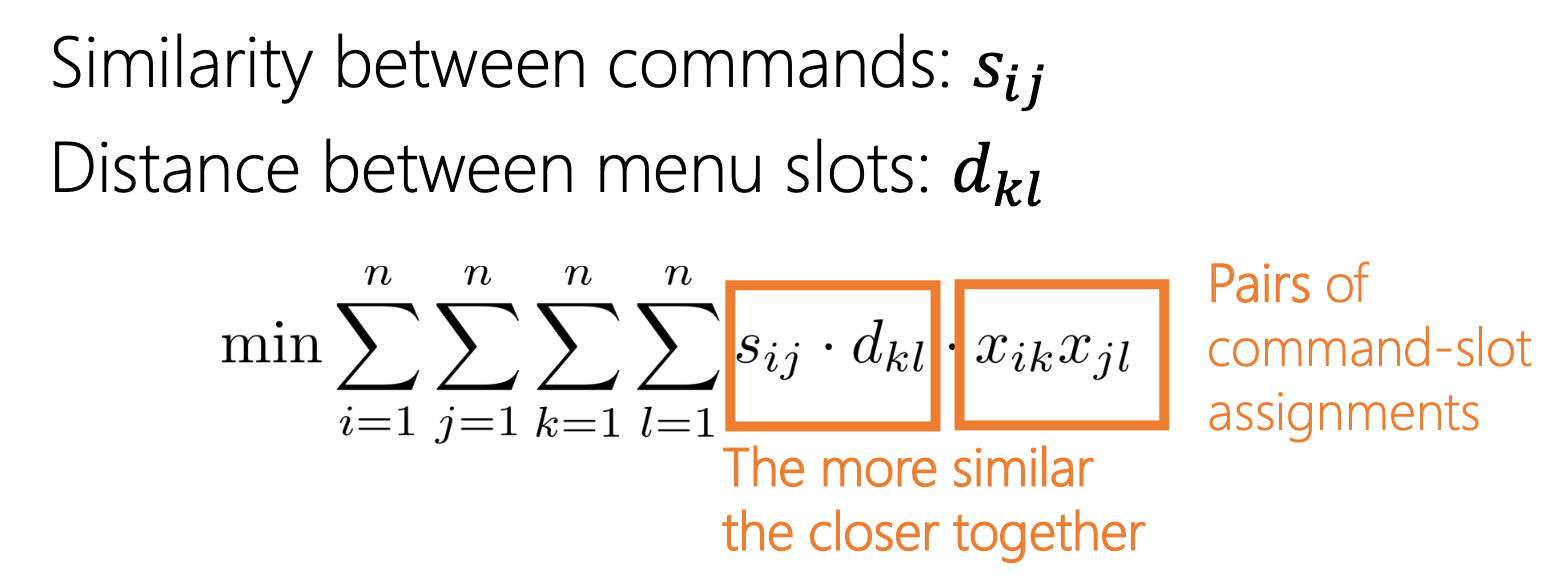
\includegraphics[width=\linewidth]{quadratic_assignment.png}
\end{center}

Is an np hard problem. Decision cost: $s_{ij} * d_{kl}$. The second part  $x_{ik} * x_{jl}$ is quadratic in the number of decisions. \medskip


\textbf{Example: The letter assignment problem} \smallskip

Question: Find best assignment of letters to keys on a smartphone to allow the fastest typing. 
Apply constraints: Each key assigned to exactly one letter, each letter assigned to exactly one key. 


\begin{center}
	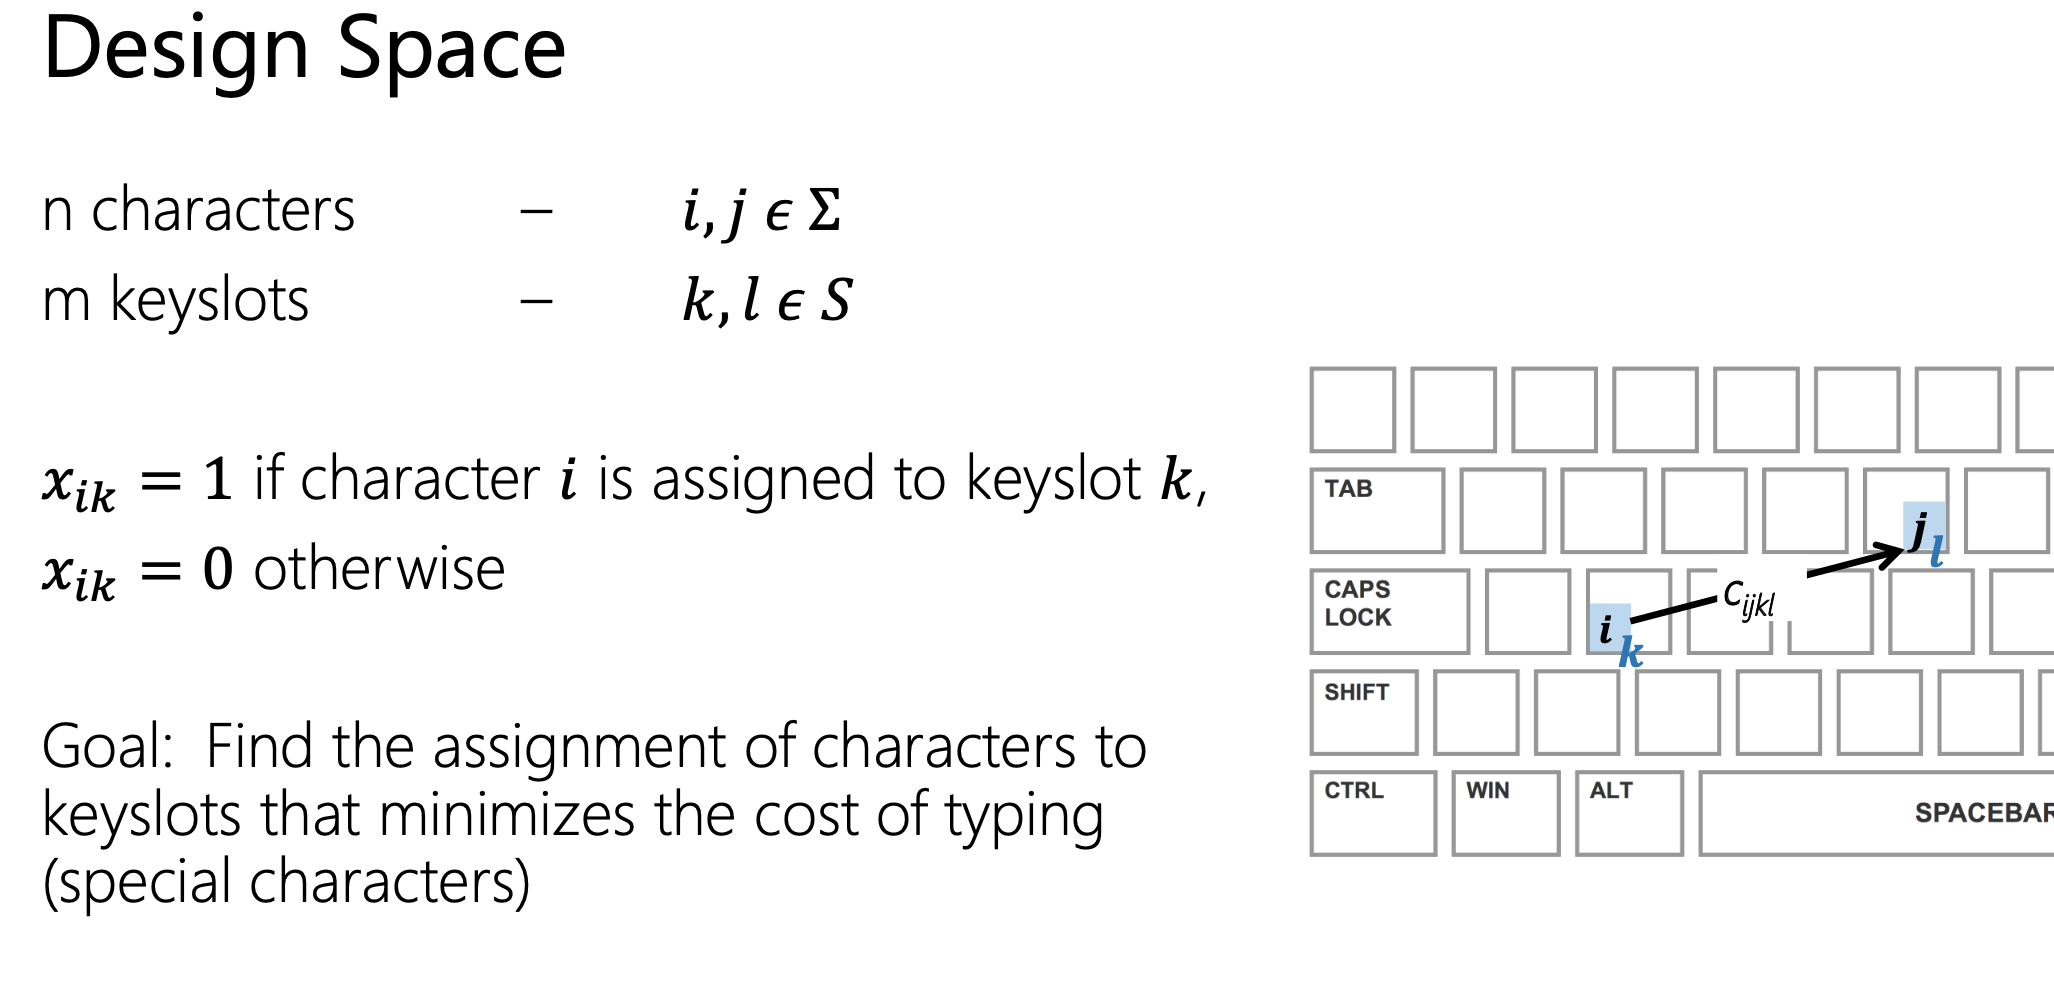
\includegraphics[width=\linewidth]{letter_example.png}
\end{center}

The goal was then to minimize the motor performance (average time to move between special characters and letters) and Ergonomics (minimize frequent extreme movements of wrist and fingers for special chars).
For Intuitiveness minimize the distance between similar special chars and also their visual similarity. Familiarity refers to redesign similar to known preferences. \medskip

\textbf{Multi-objective optimization} \smallskip

Goodness of user interface is determined by many aspects. 

\begin{itemize}[itemsep=-5pt, topsep=0pt, leftmargin=*]
	\item Performance
	\item Ergonomic and Fatigue
	\item Error prob.
	\item Mental workload
	\item learnability
	\item Accessability
	\item Subjective experience
	\item etc. 
\end{itemize}


\begin{center}
	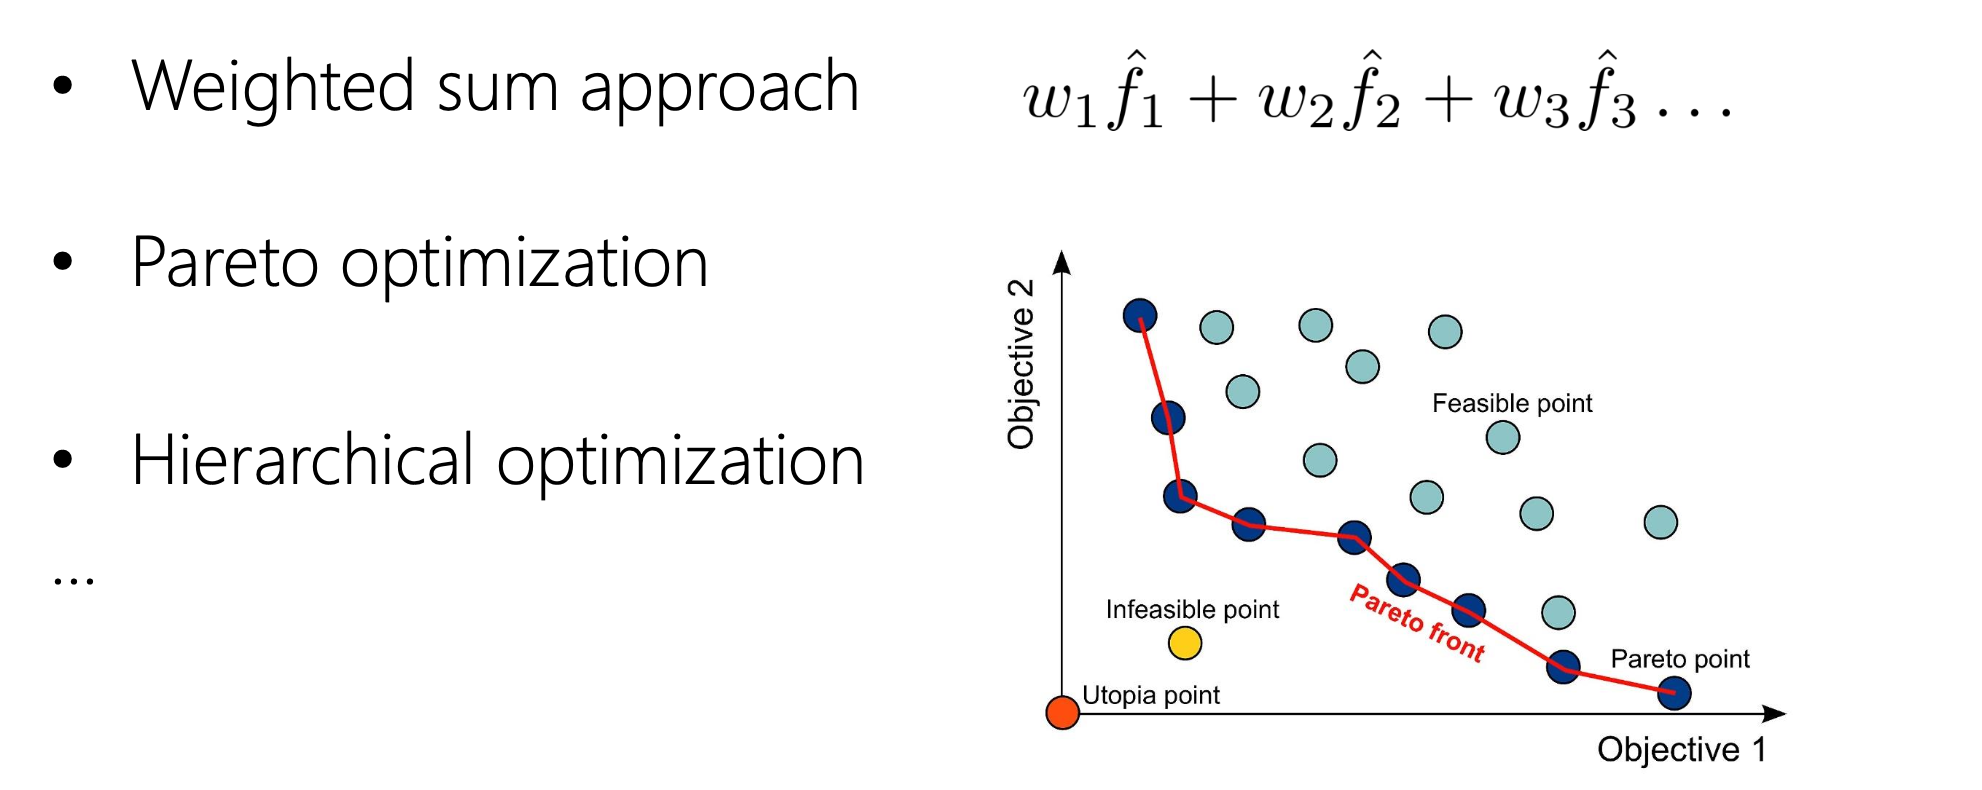
\includegraphics[width=\linewidth]{multi_objective.png}
\end{center}

\textbf{Combinatorial Optimization for User Interface Adaption} \smallskip

Optimize the UI to accomodate changes in environment, cognitive state, abilities, task, technical capabilities etc. Use different objectives such as optmize for quality and completeness. \smallskip

\textit{Element device compability}

\begin{center}
	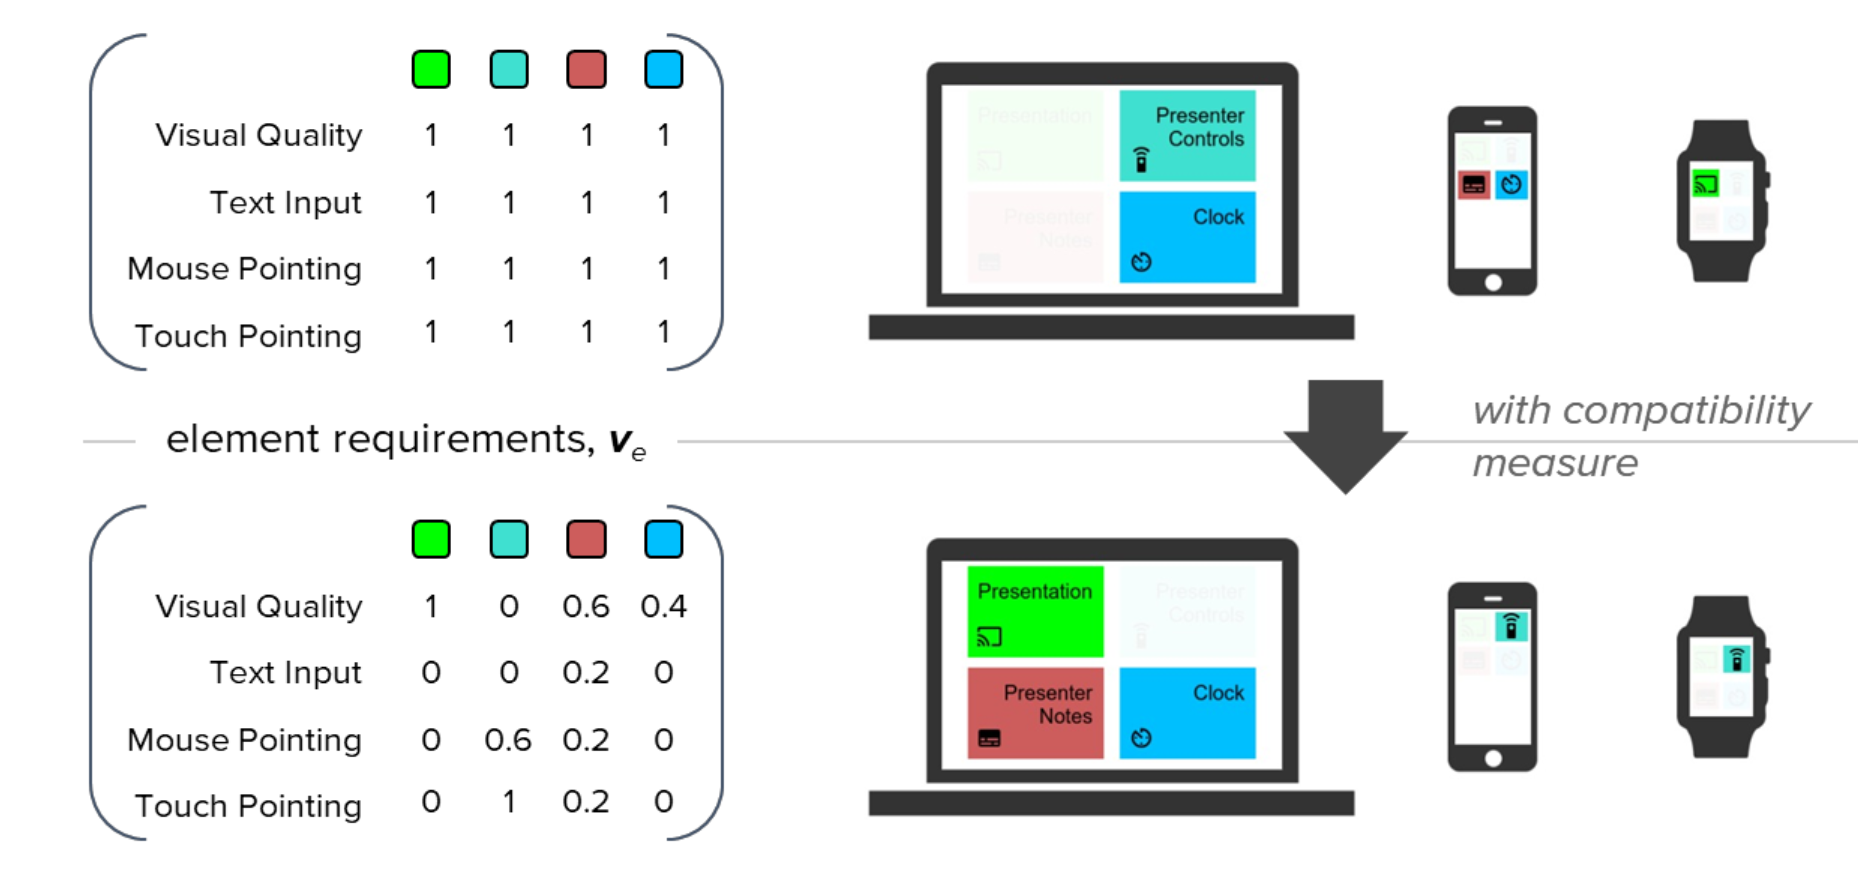
\includegraphics[width=\linewidth]{element_device_compability.png}
\end{center}

\textit{User roles}

\begin{center}
	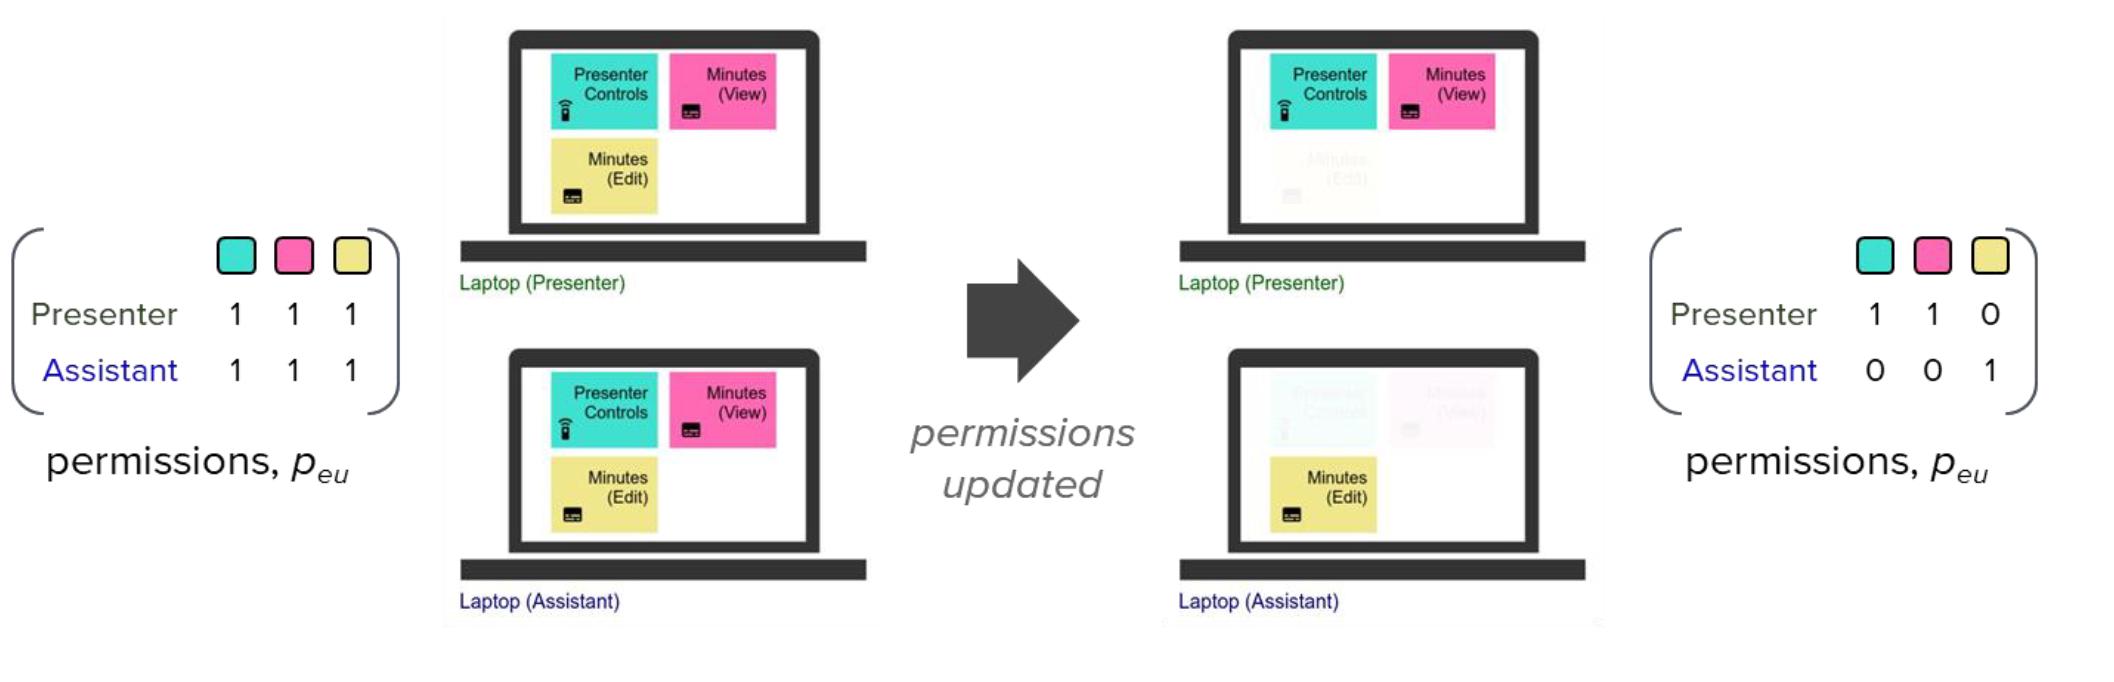
\includegraphics[width=\linewidth]{user_roles.png}
\end{center}

\textit{Cognitive Load}

\begin{center}
	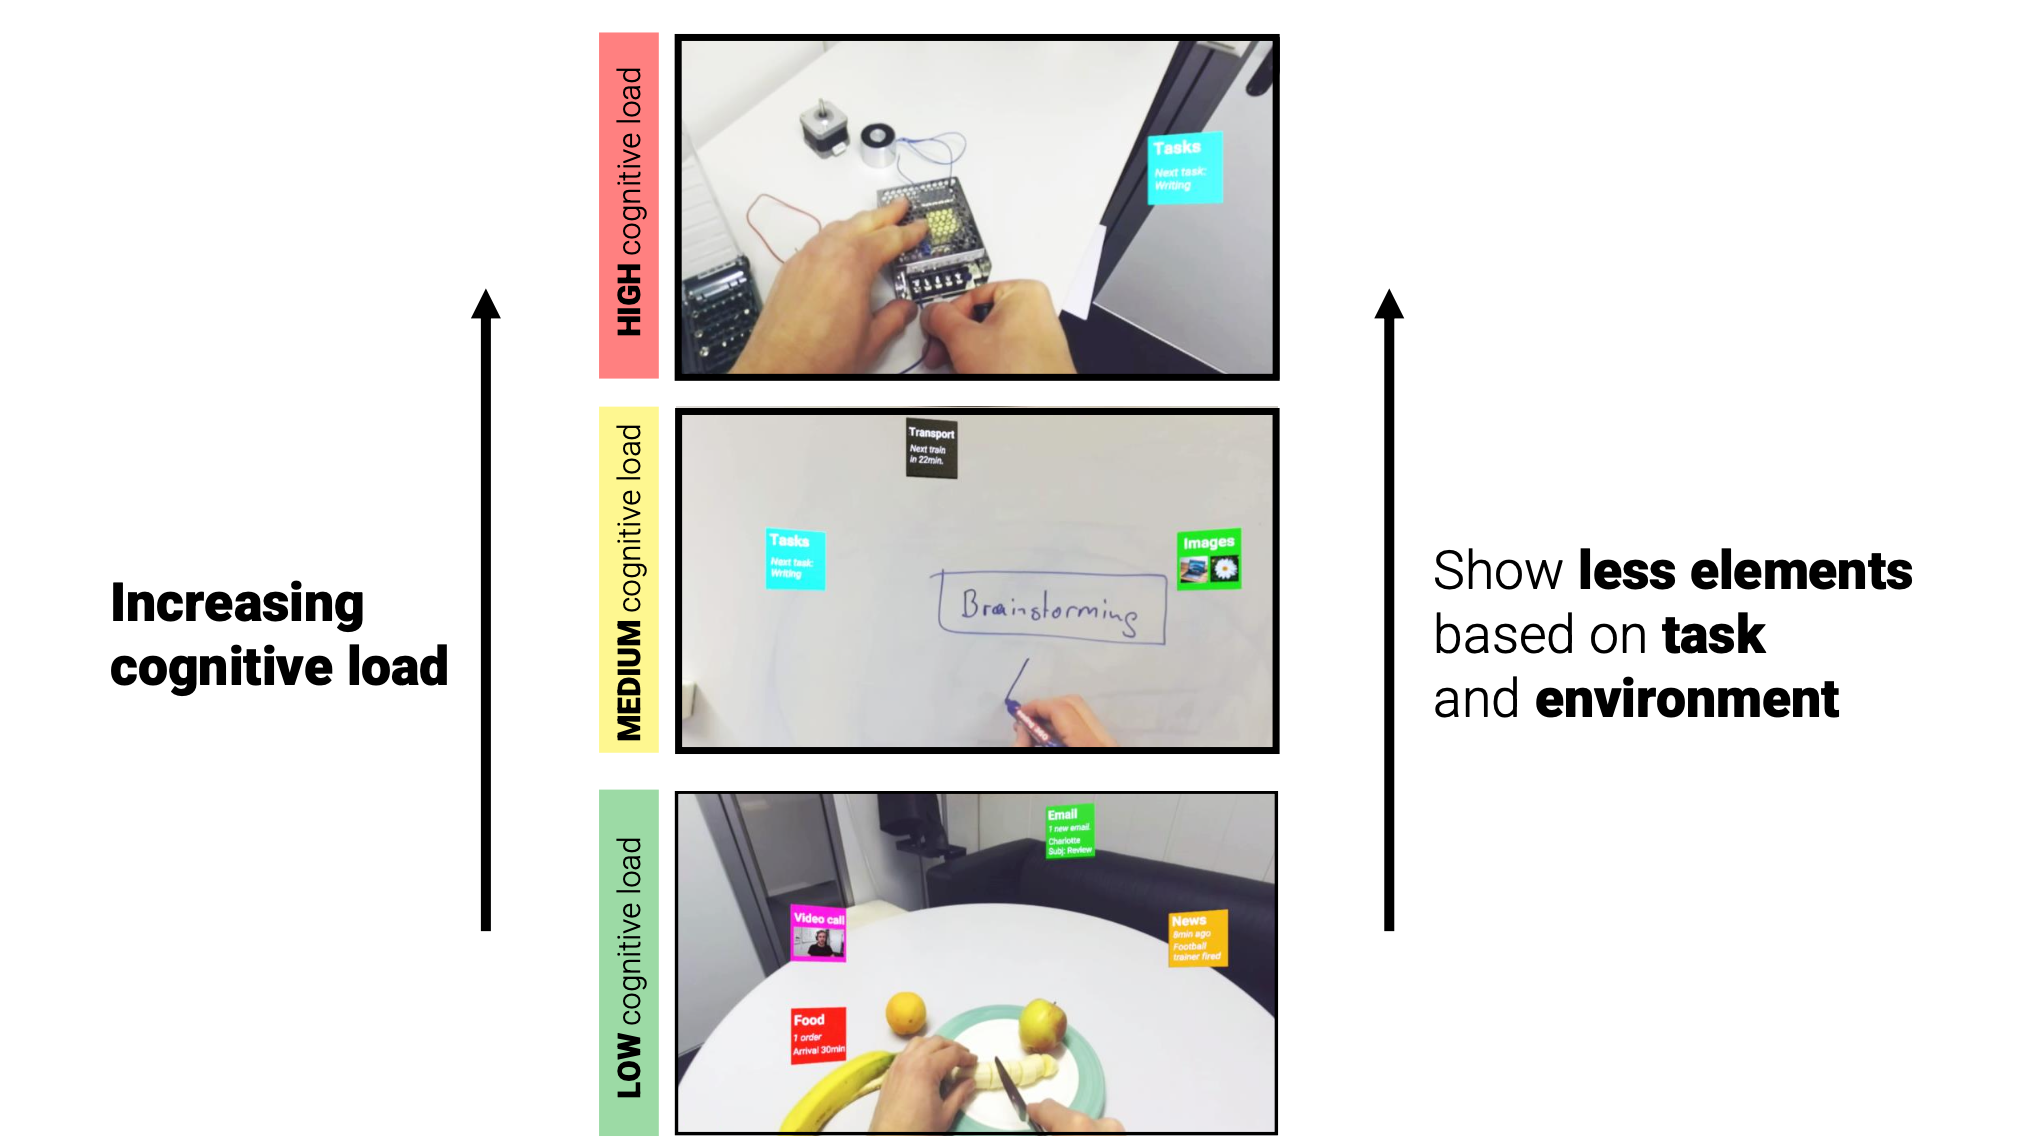
\includegraphics[width=\linewidth]{optimize_for_cognitive_load.png}
\end{center}


The idea then is to inlude cognitive load, cognitive capacity and cognitive cost to the objective function. \medskip

\textit{Optimize for environment} \smallskip

The idea is to optimize for differenct environments, e.g. screen placement, number or virtual screens etc. 
We include interaction modality, occlusion avoidance and temporal consistency in to the objective function. \smallskip

This can be done through assigning voxel containers to objects and surfaces. The objective would the be to optimally assign elements to containers. 

$x_{e,c} = \begin{cases} 1, & \text{if } e \text{ is assigned to } c \\ 0, & \text{otherwise} \end{cases}$

\begin{center}
	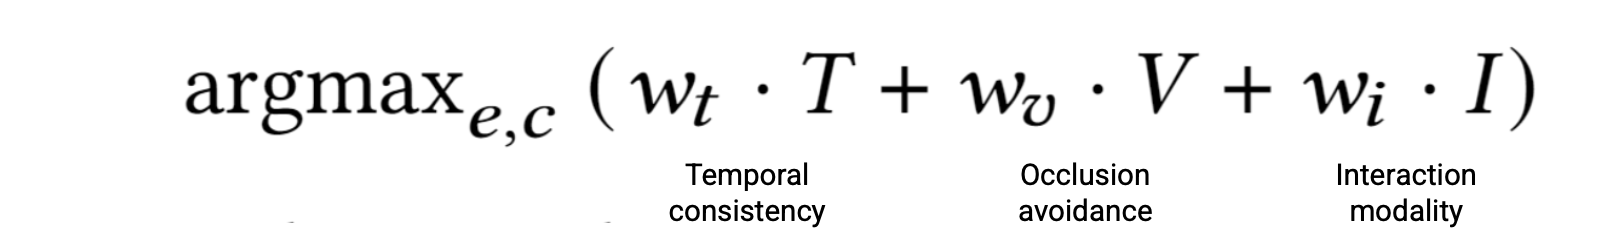
\includegraphics[width=\linewidth]{environment_formula.png}
\end{center}

\begin{center}
	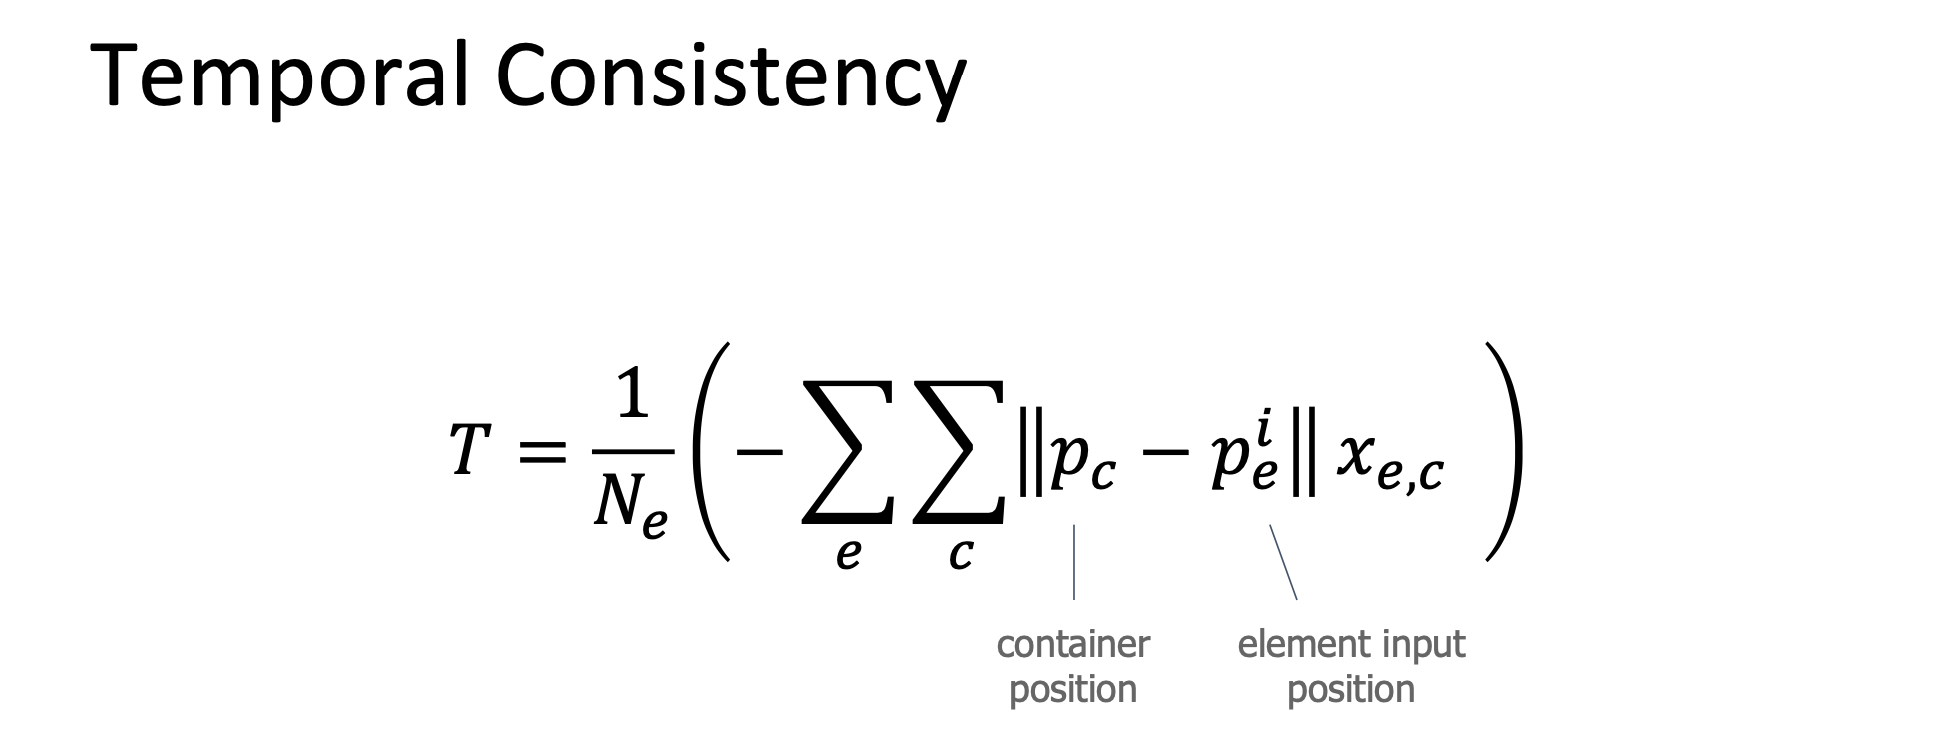
\includegraphics[width=\linewidth]{temporal_consistency.png}
\end{center}


\begin{center}
	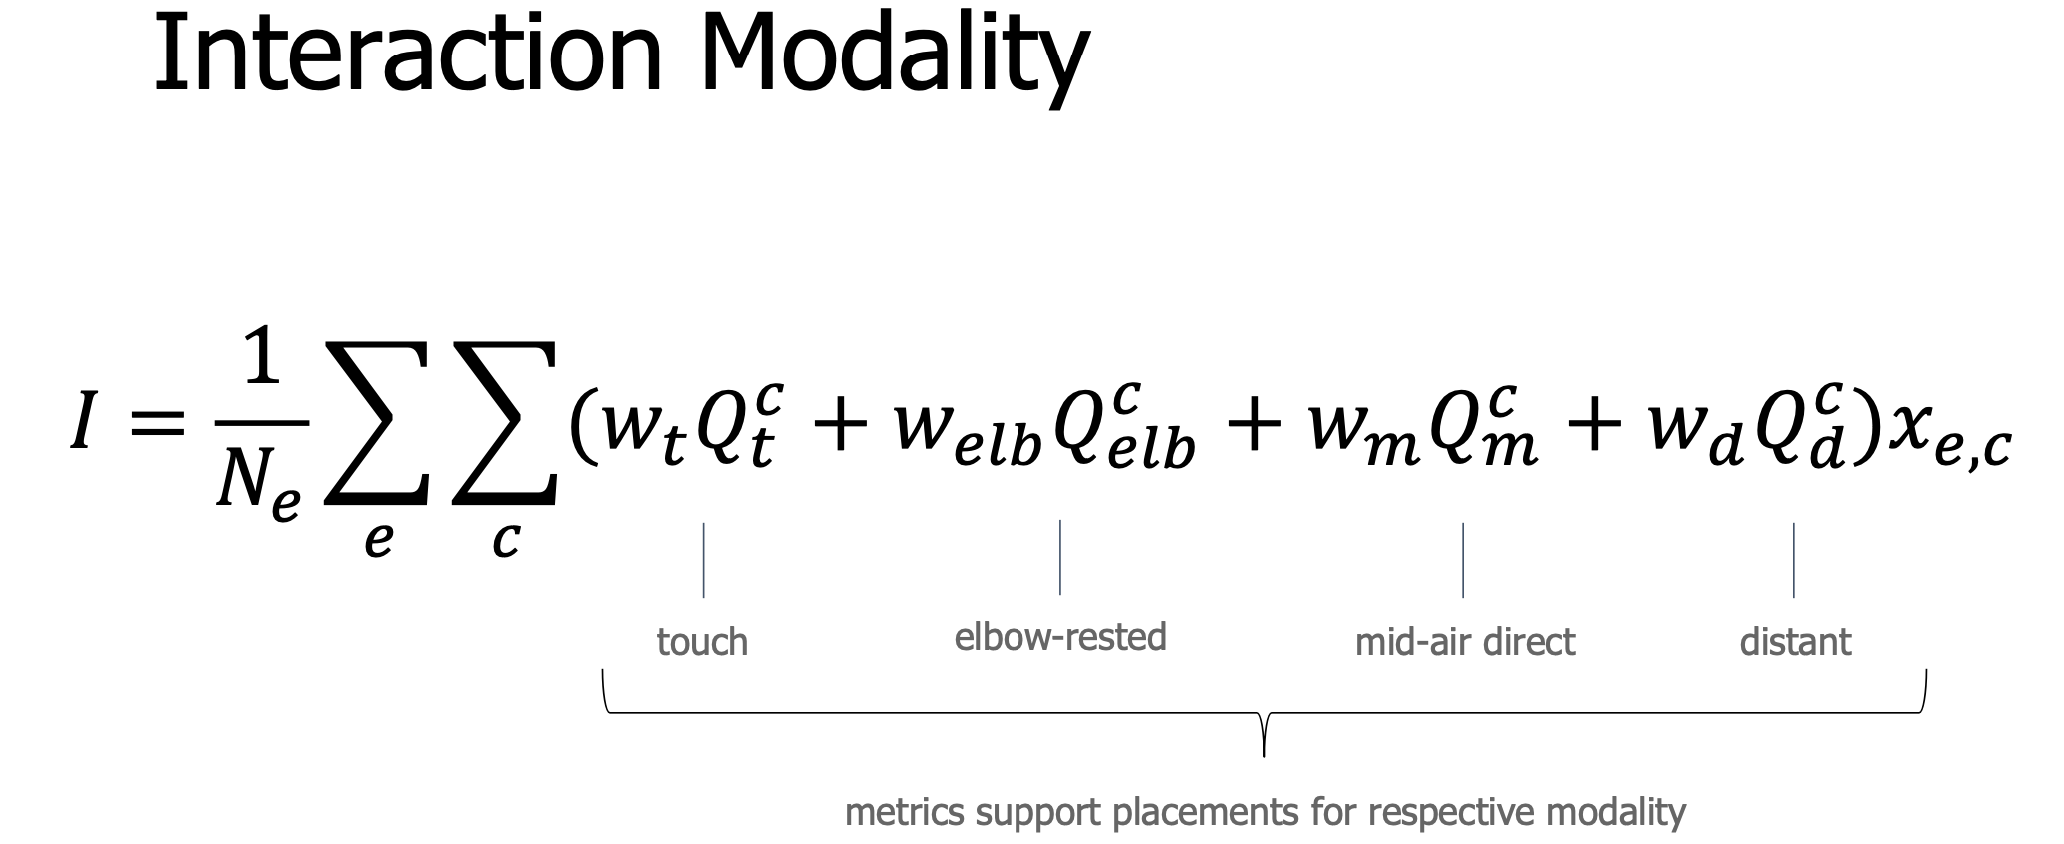
\includegraphics[width=\linewidth]{interaction_modality.png}
\end{center}

New contexts might introduce physical constraints that may render prior interface layouts unuseable. 










\section{Haptics}

\textit{Importance of haptics}

Haptics is the study of touch, force and tactile feedback in human-computer-interaction. 
Haptics feedback is everywhere and could be used for gaming, robotic surgery, education and many more. 

\begin{itemize}[itemsep=-5pt, topsep=0pt, leftmargin=*]
	\item Enhances user experience and engagement
	\item Enables more intuitive and natural interactions
	\item Adresses limitations of visual and auditory feedback
	\item Vital for accessability and inclusion
\end{itemize}\medskip



\textit{Interaction benefits}  \smallskip
\begin{itemize}[itemsep=-5pt, topsep=0pt, leftmargin=*]
	\item Increased accuracy and speed
	\item Reducing errors
	\item Eyes Free interaction
	\item Proprioceptive
\end{itemize} \medskip

\textit{Tactile} \smallskip

All about vibrations and textures.

\begin{itemize}[itemsep=-5pt, topsep=0pt, leftmargin=*]
	\item Sense of touch
	\item Goal: Stimulate skin in a programmable manner to create desired set of sensations
	\item Tactile feedback is generated by tactile device
	\item Skin based
	\item Examples: Vibration, pain, pressure, temperature
	\item Used in touchscreens, tactile displays and VR
\end{itemize}


\textit{Vibrotactile} \smallskip

\begin{itemize}[itemsep=-5pt, topsep=0pt, leftmargin=*]
	\item Subset of tactile
	\item Relies on vibrations to convey information
	\item Common in mobile devices, notifications and wearables
\end{itemize}


When designing actuators its important to consider thath different cells are in different parts of hand. 
They have different receptive fields and frequency ranges. \smallskip

Limitations of vibrotactile sensation: Broad localization of the sensation, superficial feedback and thus the strength of the vibration may be perceived differentyl based on the area of skin in contact with mounting pressure. 
\medskip

\textit{Kinesthetic} \smallskip

Very accurate receptors in muscles, joint and skin. All about movement and force.  \smallskip

Passive Kinesthetic (Force feedback): Perception of resistance or force, it requires human motion/input. Examples are surgical simulators or controllers. 


Limitations to passive kinesthetic: 


\begin{itemize}[itemsep=-5pt, topsep=0pt, leftmargin=*]
	\item Hard to design
	\item Often cumpersome
	\item User needs to provide inpput
	\item Limited part of how we perceive the world
\end{itemize}


\textit{Active Kinesthetic} \smallskip

Focuses on the sense of body movement and position. Relevant in motion simulators, exoskeletons and teleoperation systems. 


Limitations to passive kinesthetic: 


\begin{itemize}[itemsep=-5pt, topsep=0pt, leftmargin=*]
	\item Hard to design
	\item Often cumpersome
	\item Expensive
	\item Limited part of how we perceive world
\end{itemize}




\section{Computational Rationality}

Comp. Rationality converges ideas from AI, robotics, cognitive science and neurosciences. 

It refers to computational principles for:
\begin{enumerate}[itemsep=-5pt, topsep=0pt, leftmargin=*]
    \item Identifying decisions with highest expected utility, while taking into consideration the costs of computation in complex real-world problem, where calculations can only be approximated.
    \item Implementing bounded optimality in humans. 
\end{enumerate}

\textbf{Why User Models}

\begin{itemize}[itemsep=-5pt, topsep=0pt, leftmargin=*]
	\item Used as test to help in creation and validation of new HCI theories
	\item Helps design more robust interaction, with improved safety and accessibility
	\item Reduce financial, temporal and human costs of usability testing
	\item Helps take advantage of advances in other engineering disciplines
	\item Advance next generation of intelligent interactive systems
\end{itemize}

\textit{Limitations to Model human processor} \smallskip

\begin{itemize}[itemsep=-5pt, topsep=0pt, leftmargin=*]
	\item does not learn, adapt, generalize and has othe tradeoffs
\end{itemize}
Interaction is not equal to emerging behavior. After initial task has failed/succeded, there is no adaptive behavior or reorganization without explicit instruction.

\textit{Complexities of real-world tasks} \smallskip

\begin{itemize}[itemsep=-5pt, topsep=0pt, leftmargin=*]
	\item Generalization: Go from precious episodes to an unseen one
	\item Latent learning: Adapting to distal changes in environment
	\item Planning: Sequencing actions while considering long-term effects on reward
	\item Compositionality: Good solution require putting together partial solutions cleverly
	\item Exploration/exploitation: Knowing when to learn the structure of task /environment vs when to exploit it
	\item Uncertainty: Knowledge can be incomplete or incorrect
	\item Resource limitations: Limited time and capabilities
	\item Curse of dimensionality: A very large number of possibilities
\end{itemize}

\begin{center}
	\includegraphics[width=\linewidth]{policy_estimation_view.png}
\end{center}


\textbf{Optimal Policy}

Is supposed to look at emerging bahavior component. \medskip

\textit{Interactions as a sequential decision-making process} \smallskip

\begin{center}
	\includegraphics[width=\linewidth]{book_flights.png}
\end{center}

\begin{center}
	\includegraphics[width=\linewidth]{interaction_sequential.png}
\end{center}


\textit{Reinforcement Learning (RL)} \smallskip

RL is an interdisciplinary area of machine learning and optimal control concerned with how an intelligent agent ought to take actions in a dynamic environment to maximize the cumulative reward. 

\begin{center}
	\includegraphics[width=\linewidth]{reinforcement_learning.png}
\end{center}

Example for state, action and rewards: 
\begin{center}
	\includegraphics[width=\linewidth]{example_RL.png}
\end{center}

What is the optimal action to take given a state? \smallskip


\textit{Difference from RL to other ML paradigms} \smallskip

\begin{minipage}{\linewidth} 
	\centering
	\includegraphics[width=0.45\linewidth]{HCI.png}
	\quad 
	\includegraphics[width=0.45\linewidth]{machine_learning.png}
  \end{minipage}

\begin{itemize}[itemsep=-5pt, topsep=0pt, leftmargin=*]
	\item No supervisor, only a reward signal
	\item feedback is delayed, not instantaneous
	\item Time really matters (sequential, non i.i.d data)
	\item Agent's actions affect the subsequent data it receives
\end{itemize}

\textit{Markov Decision Process} \smallskip

Tuple: $\{S, A, T, R, \gamma\}$

\begin{itemize}[itemsep=-5pt, topsep=0pt, leftmargin=*]
	\item S: A finite set of states (what letters have I typed so far)
	\item A: A finite set of actions (what letter do I type next, what muscle do I activate)
	\item T: Transition matrix: $p(s', a, s)$ given state and action, what is the prob of the next state
	\item R: Reward $R(s', a, ss)$ the immediate reward of taking the action $a$ in state $s$. 
	\item $\gamma \in [0, 1)$: the discount factor
\end{itemize}


\textit{Optimal action given a state} \smallskip

Policy is the agent's bahavior. It maps a state to an action to maximize the cumulative reward. 

The goal is to find an optimal policy: $\pi$ \smallbreak

\textit{Value Function} \smallskip

Value function is a prediction of future reward. Used to evaluate the goodness/badness of states. Therefore select between actions. 

$$V_{\pi}(s) = E_{\pi}[R_{t+1} + \gamma R_{t+2} + \gamma^2 R_{t+3} + ... | s_{t} = s]$$

\textit{On Rewards} \smallskip
It is a scalar feedback and describes how well an agent is doing at step t. 


The reward hypothesis states that all goals can be described by the maximization of the expected cumulative reward. 

\textbf{Bounded Rationality}

Supposed to look at Human-likeness.

\textit{Comparison with Standard RL} \smallskip

\begin{center}
	\includegraphics[width=\linewidth]{comparison_RL.png}
\end{center}

\textit{Internal vs External Environmen} \smallskip

\begin{itemize}[itemsep=-5pt, topsep=0pt, leftmargin=*]
	\item Humans acit in the external environment via their internal environment
	\item External environment: The world
	\item Internal environment: Cognition
	\item Agent: Decison maker
\end{itemize}

Interaction emerges as adaption within internal and external bounds. 


\begin{center}
	\includegraphics[width=\linewidth]{bounded_optimality.png}
\end{center}


\begin{center}
	\includegraphics[width=\linewidth]{ml_and_bounds.png}
\end{center}




\begin{center}
	\includegraphics[width=\linewidth]{cognitive_architecture.png}
\end{center}


\textbf{Key cognitive capacities in HCI} \smallskip

\begin{itemize}[itemsep=-5pt, topsep=0pt, leftmargin=*]
	\item (Suvervisory Control): Adaptively deciding goals, allocating cognitive resources to tasks, and changing course of action when required. 
	\item Memory: Forming, maintaining and accessing beliefs about objects that are not directly perceivable
	\item Attention: Selectively processing some part of the perceptual failed
	\item Reasoning: Applying transformation rules to beliefs to form new beliefs
	\item Gathering information and choosing between options
\end{itemize}

\textit{General props of Human Cognition} \smallskip

\begin{itemize}[itemsep=-5pt, topsep=0pt, leftmargin=*]
	\item Goal-oriented
	\item Adapts
	\item Learns
	\item Carries out computations on representations
	\item Is limited
	\item Requires energy and effort
\end{itemize}


\textit{1. Cognition is goal oriented} \smallskip

How do we choose what stimuli to direct our cognitive resources on. We use cognitive control to decide to which goal we direct thinking and action.

\begin{itemize}[itemsep=-5pt, topsep=0pt, leftmargin=*]
	\item Setting goals
	\item Directing resources and Attention
	\item Multitasking
	\item Task-switching
	\item Inhibiting distracting ideas
\end{itemize}

\textit{2. Cognition Adapts} \smallskip

Systems used by people and the way work is carried out changes all the time. 
\begin{itemize}[itemsep=-5pt, topsep=0pt, leftmargin=*]
	\item Cognitive, motor and perceptual processes need to adapt constantly
	\item Update old beliefs with new ones
	\item Update old plans and form new ones
	\item Cognition is not only reacting to environments but also actively finding ways to function better
\end{itemize}


\textit{3. Cognition Learns} \smallskip

Computers are complex but opaque systems. We need internal representations to control them and need to have multiple memory systems to that end. 
It learns to use external aids. 

Cognition also learns how to use external aids such as notes calculators etc. to augment our abilities. This changes the way we use cognition in interaction. 
Example is GUIs that have lead to forget commands in memory. 


Example: Menu interaction of non-sighted users
\begin{center}
	\includegraphics[width=\linewidth]{Cognition_learns_example.png}
\end{center}


\textit{4. Cognition computes based on internal representations} \smallskip

 Cognition can reason about things that are not directly perceivable. It uses internal models of reality to reason, formulate goals and plans.

 Examples are metaphors to help users understand an UI. Desktop metaphor uses spatial concepts that are rooted in everyday physical experiences. 

\textit{5. Cognition is limited \& costs energy} \smallskip

\begin{itemize}[itemsep=-5pt, topsep=0pt, leftmargin=*]
	\item Visual attention is spactially limited (periphery vs foveal region)
	\item Working memory is capacity-limited (only few mental representations active at a time, typically working memory is limited to 2-4 items)
	\item Forgetting occurs in long-term memory (we cannot remember everything we have experiences and thus forget details)
	\item Capacity for abstract reasoning and planning is limited (only think few steps ahead)
\end{itemize}


\textit{Perception} \smallskip

Perception is needed to regulate actions:
\begin{itemize}[itemsep=-5pt, topsep=0pt, leftmargin=*]
	\item UIs communicate their state via perception
	\item Visual, auditory and tactile perception each have own characteristics and roles in HCI
\end{itemize}

\begin{center}
	\includegraphics[width=\linewidth]{perception.png}
\end{center}


\textit{Elementary perceptual Tasks} \smallskip

\begin{itemize}[itemsep=-5pt, topsep=0pt, leftmargin=*]
	\item Discrimination: telling whether a difference occurs in sensory data
	\item Detection: telling whether an event of interest occurs or not
	\item Recognition: Categorizing a stimulus as something
	\item Estimation: estimate property of an object of event in the environment
	\item Search: localizing an object of interest
\end{itemize}

\textbf{Gaze-based Interaction} \smallskip

Proble of selecting items on a computer with eye movements and fixations. These eyemovements obey Fitt's Law. 
Movement time of the eyes is proportional to distance and inversely proportional to size of the target.


\begin{center}
	\includegraphics[width=\linewidth]{Gaze_based_interaction.png}
\end{center}



\textit{Comparison with Cognitive Architectures}


\begin{center}
	\includegraphics[width=\linewidth]{comparison_cognitive_architectures.png}
\end{center}














\end{multicols*}
\end{document}

% ____ FOOTER ______________________________________________________
% Content and Template: 
% original by Benjamin Gantenbein (bgantenbein@ethz.ch), 2023
